\documentclass[11pt]{article}
% packages
\usepackage[utf8]{inputenc}
\usepackage[french]{babel}
\usepackage[T1]{fontenc}
\usepackage{geometry}
\usepackage[pdftex]{graphicx}
\usepackage{graphicx}
\usepackage{tabularx}
\usepackage{dsfont}
\usepackage{multirow}
\usepackage{amsmath,amsfonts,amssymb}
\usepackage{subcaption}
\usepackage{authblk}
\usepackage{placeins}
\usepackage{epigraph}


\usepackage{lscape}
\usepackage{rotating}
\usepackage{longtable}
\usepackage{array, booktabs, ltablex, makecell, threeparttablex}

%hyperlinks options
\usepackage{hyperref}
\hypersetup{colorlinks=true,linkcolor=blue,filecolor=magenta,urlcolor=cyan,citecolor=cyan}
%bib options
\usepackage[backend=biber,style=authoryear,bibstyle=authoryear,natbib=true,
giveninits=true,uniquename=false,uniquelist=false,% firstinits=false,
maxcitenames=2,date=year, maxbibnames=99,url=false]{biblatex}
\geometry{left=20mm, top=20mm, right=20mm}
%float barrier
\usepackage{placeins}
 \addbibresource{Thèse.bib}
\title{Chapitre 2 : Collecte et caractérisation des données de crue à Beaucaire}
\author{Mathieu}

\begin{document}
\maketitle


\tableofcontents


\newpage 

%\section{Introduction}

\section{Hydrométrie du Rhône à Beaucaire de 1816 à aujourd'hui}
\label{sec:hydrometrie}

\paragraph{} Le passé de Beaucaire, du XVII\textsuperscript{ème} au XIX\textsuperscript{ème} siècle était indéniablement tourné vers le commerce fluvial. La foire de Beaucaire, d'importance européenne, attirait alors des marchands venus des quatre coins de la Méditerranée (figure \ref{fig:foire}). La ville de Beaucaire était considérée comme « \textit{la capitale française des marchandises} » \citep{leon_vie_1953} grâce à sa proximité avec la mer et les échanges fluviaux rendus possibles par son port sur le Rhône. L'attention des beaucairois était alors tournée continuellement vers le fleuve et ses caprices. Les crues et étiages fréquents perturbaient le commerce fluvial, source principale des revenus Beaucairois avant l'avènement du chemin de fer. A cette époque, Beaucaire et Tarascon étaient reliées par un pont de bateaux, qui, jusqu'à la construction d'un pont en pierre en 1830, servait à passer d'une ville à l'autre. Ce pont était régulièrement détruit par les crues, comme en 1745 : « \textit{le pont de bateaux de Tarascon alla heurter et emporter celui d'Arles} » \citep{anibert_annales_1764}. Du fait de cet intérêt majeur pour le fleuve, le Rhône à Beaucaire fut l'une des premières stations limnimétriques françaises avec des relevés continus dès le début du XIX\textsuperscript{ème} siècle. 


\begin{figure}[h]
		\centering
            \begin{subfigure}{0.49\linewidth}
            \centering
            	\includegraphics[width=1\linewidth]{Figures/foire4.jpg}\hfill
            	\caption{}
            	\label{subfig:foire1}
            \end{subfigure}
            \begin{subfigure}{0.49\linewidth}
            \centering
            	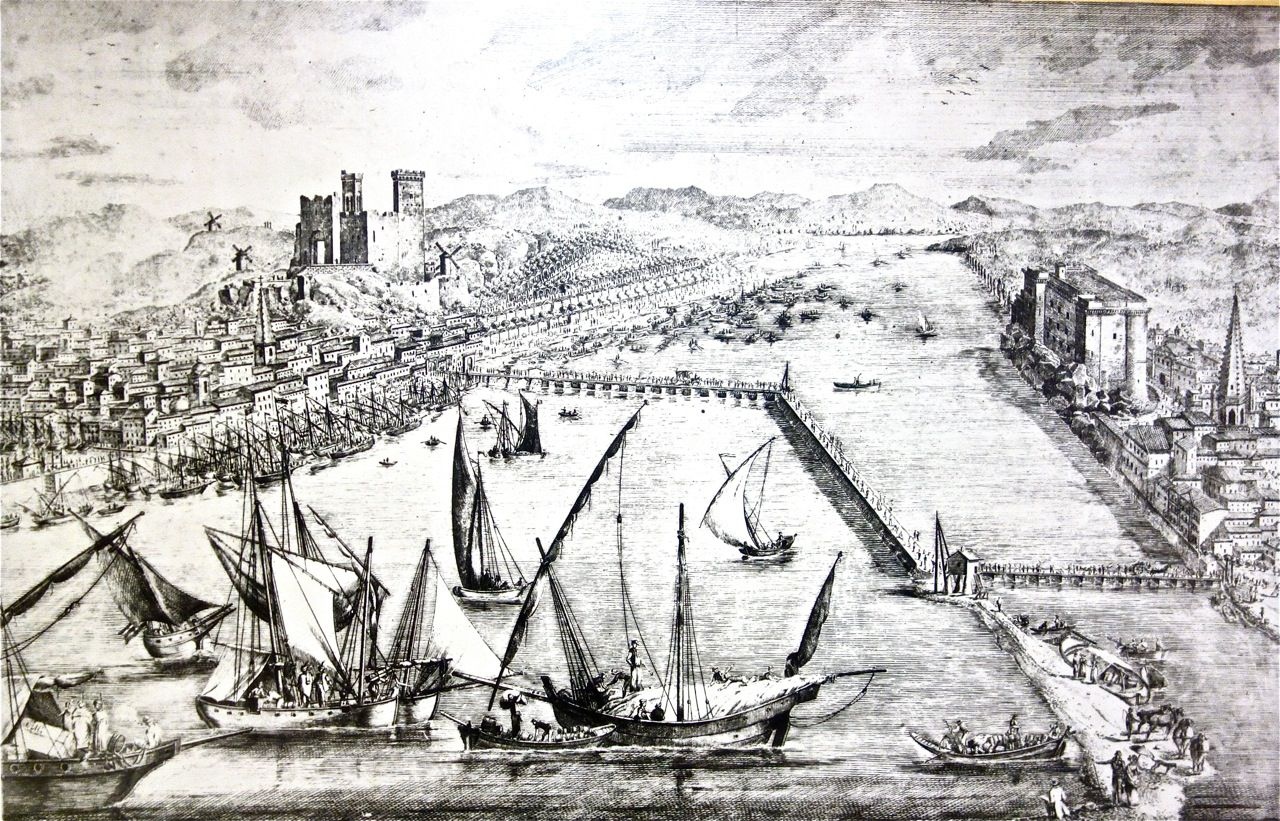
\includegraphics[width=1\linewidth]{Figures/foire5.jpg}
            	\caption{}
           		\label{subfig:foire2}
            \end{subfigure}
\caption{(a) « \textit{Vue de la foire de Beaucaire avec une partie de la ville de Tarascon} », Basset André (1749). On distingue la ville de Beaucaire sur la droite et Tarascon sur l'autre rive. 
(b) Pont de bateaux reliant Beaucaire à Tarascon lors de la foire, auteur inconnu (XVIII\textsuperscript{ème} siècle). Le pont était alors régulièrement détruit lors des crues, empêchant toute communication entre les deux villes.}
\label{fig:foire}
\end{figure}

	\subsection{Contexte hydrologique et hydrométrique}
	
	\paragraph{} Le Rhône à Beaucaire draine un bassin versant de 95 590 km² et son module est de 1680 m\textsuperscript{3}/s (1920-2023) \citep{medd_banque_2021}. La station hydrométrique de Beaucaire est la station la plus à l'aval du Rhône dit "complet" car elle est située 5 km à l'aval de la confluence avec le Gardon (dernier affluent significatif du Rhône), et 10 km à l'amont de la diffluence qui donne naissance au Petit-Rhône et au Grand-Rhône (figure \ref{fig:BV}). Il s'agit donc de la station mesurant le débit le plus important du fleuve, mais également de France, le Rhône étant le premier fleuve français en terme de débit (à l'exception du Rhin qui est frontalier). Au delà de son important débit, le Rhône est un fleuve complexe par la diversité de ses apports, comme décrit par \citet{parde_regime_1925}, il comporte « \textit{ une infinité de nuances et de contrastes, la Massa, l'Arve, l'Isère, la Durance, l'Ain, la Saône, l'Ardèche, c'est-à-dire des cours d'eau appartenant à toutes les catégories qu'on puisse trouver en Europe occidentale. [...] Ainsi, c'est par une carrière agitée que le petit torrent glaciaire de Gletsch devient le fleuve majestueux de Beaucaire, tour à tour ou en même temps nival et séquanien, océanique et méditerranéen, pondéré ou sujet aux plus déconcertants accès de démence} ». À Beaucaire, les signatures des affluents alpins, océaniques, méditerranéens et cévenols se mélangent pour donner naissance à un régime hydrologique qu'il est difficile de classer dans une catégorie (figure \ref{fig:Regime}). Il en est de même pour les crues, qui sont le reflet de la complexité de ses apports : « \textit{Il est violent par son courant encore inapaisé tout près de la Méditerranée, par ses crues de plus en plus nombreuses, désordonnées et massives, à mesure qu'il approche du terme de son cours} » \citep{parde_regime_1925}. 

	\paragraph{} Au cours des deux derniers siècles, trois crues apparaissent comme particulièrement marquantes. Tout d'abord l'événement du 3 novembre 1840 est probablement le plus important depuis le début du XIX\textsuperscript{ème} siècle. Il est décrit par \citet{parde_regime_1925} comme \textit{"l'événement météorologique le plus grandiose et le plus déconcertant qui se soit jamais produit dans le bassin du Rhône"}. Les dégâts sont généralisés : le centre ville de Lyon est sous les eaux, la concomitance avec la crue de la Durance entraine de nombreux dégâts à Avignon et la Camargue est complètement inondée suite à de nombreuses brèches dans les digues. \citet{parde_regime_1925} donne une estimation de débit à 13 000 m\textsuperscript{3}/s à Beaucaire. Vient ensuite la crue du 31 mai 1856 qui touche non seulement le Rhône, mais également de nombreux cours d'eau français dont la Loire. \citet{parde_regime_1925} la décrit comme "\textit{la plus simple et la plus brutale des crues générales du Rhône}" et estime son débit à Beaucaire à 12 500 m\textsuperscript{3}/s. A nouveau, les dégâts sont colossaux de Lyon à la mer. Ces deux crues de période de retour supérieures à 100 ans sont encore aujourd'hui des références pour l'estimation du risque d'inondation. Jusqu'en décembre 2003, aucun événement ne s'en était réellement approché et les risques de débordements majeurs et de ruptures de digues avaient été peu à peu oubliés. Avec ses 11 500 m\textsuperscript{3}/s qui correspondent à une période de retour centennale \citep{medd_debit_2005}, la crue de 2003 a ravivé les craintes des populations provençales. Au cours de l'événement, plusieurs digues supposées résister à des niveaux similaires à ceux de 1856 cèdent et provoquent l'inondation des foyers de plus de 8000 personnes. Suite à cet événement, une stratégie d'aménagement pour la prévention du risque inondation est mise en place (\url{www.plan-rhone.fr}) et de nombreuses digues sont rehaussées, notamment à l'aval de Beaucaire \citep{symadrem_programme_2012}. 
	
	\begin{figure}[h!]
	\centering
		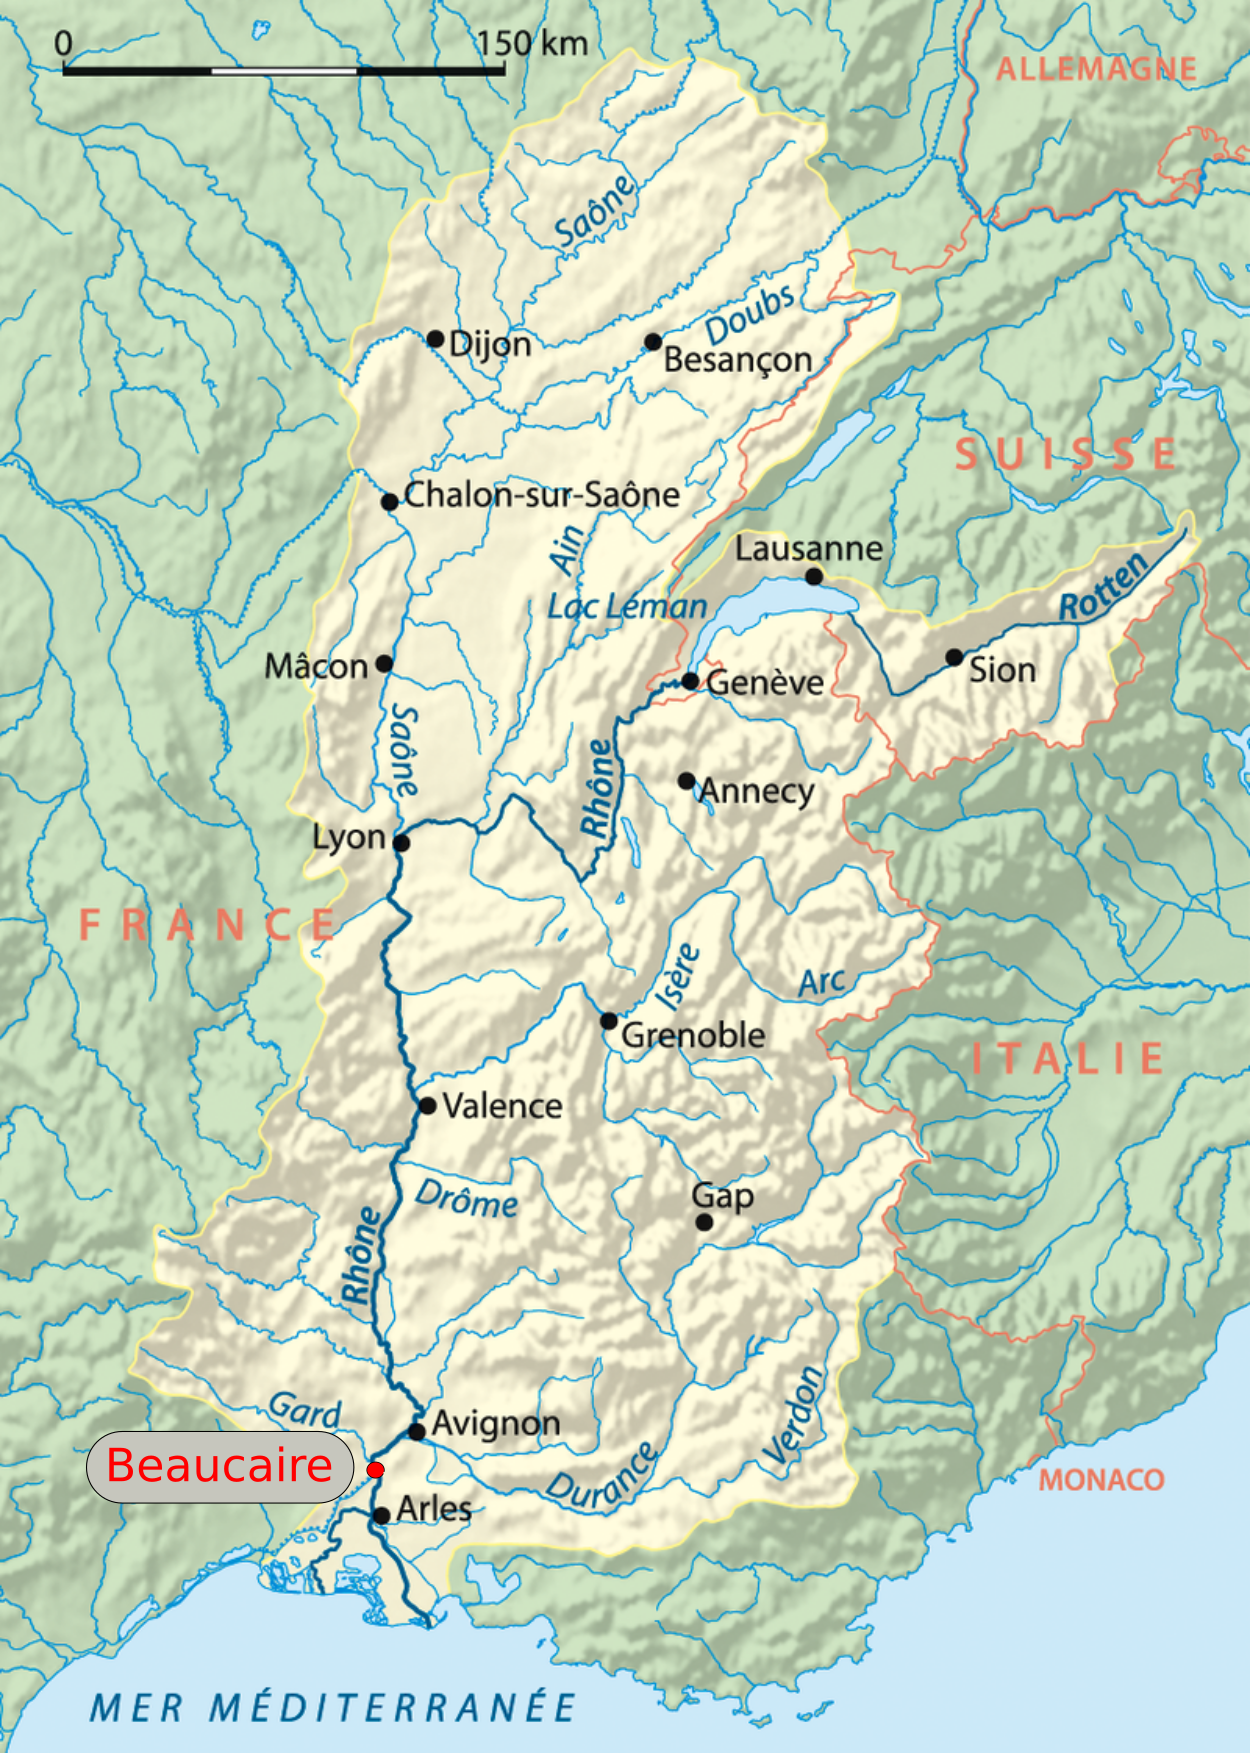
\includegraphics[width=.5\linewidth]{Figures/Rhone_bassin_versant.png}
        \caption{Bassin versant du Rhône. La ville de Beaucaire est indiquée en rouge (www.openstreetmap.org)}	
		\label{fig:BV}
	\end{figure}
	
	\begin{figure}[h!]
	\centering
		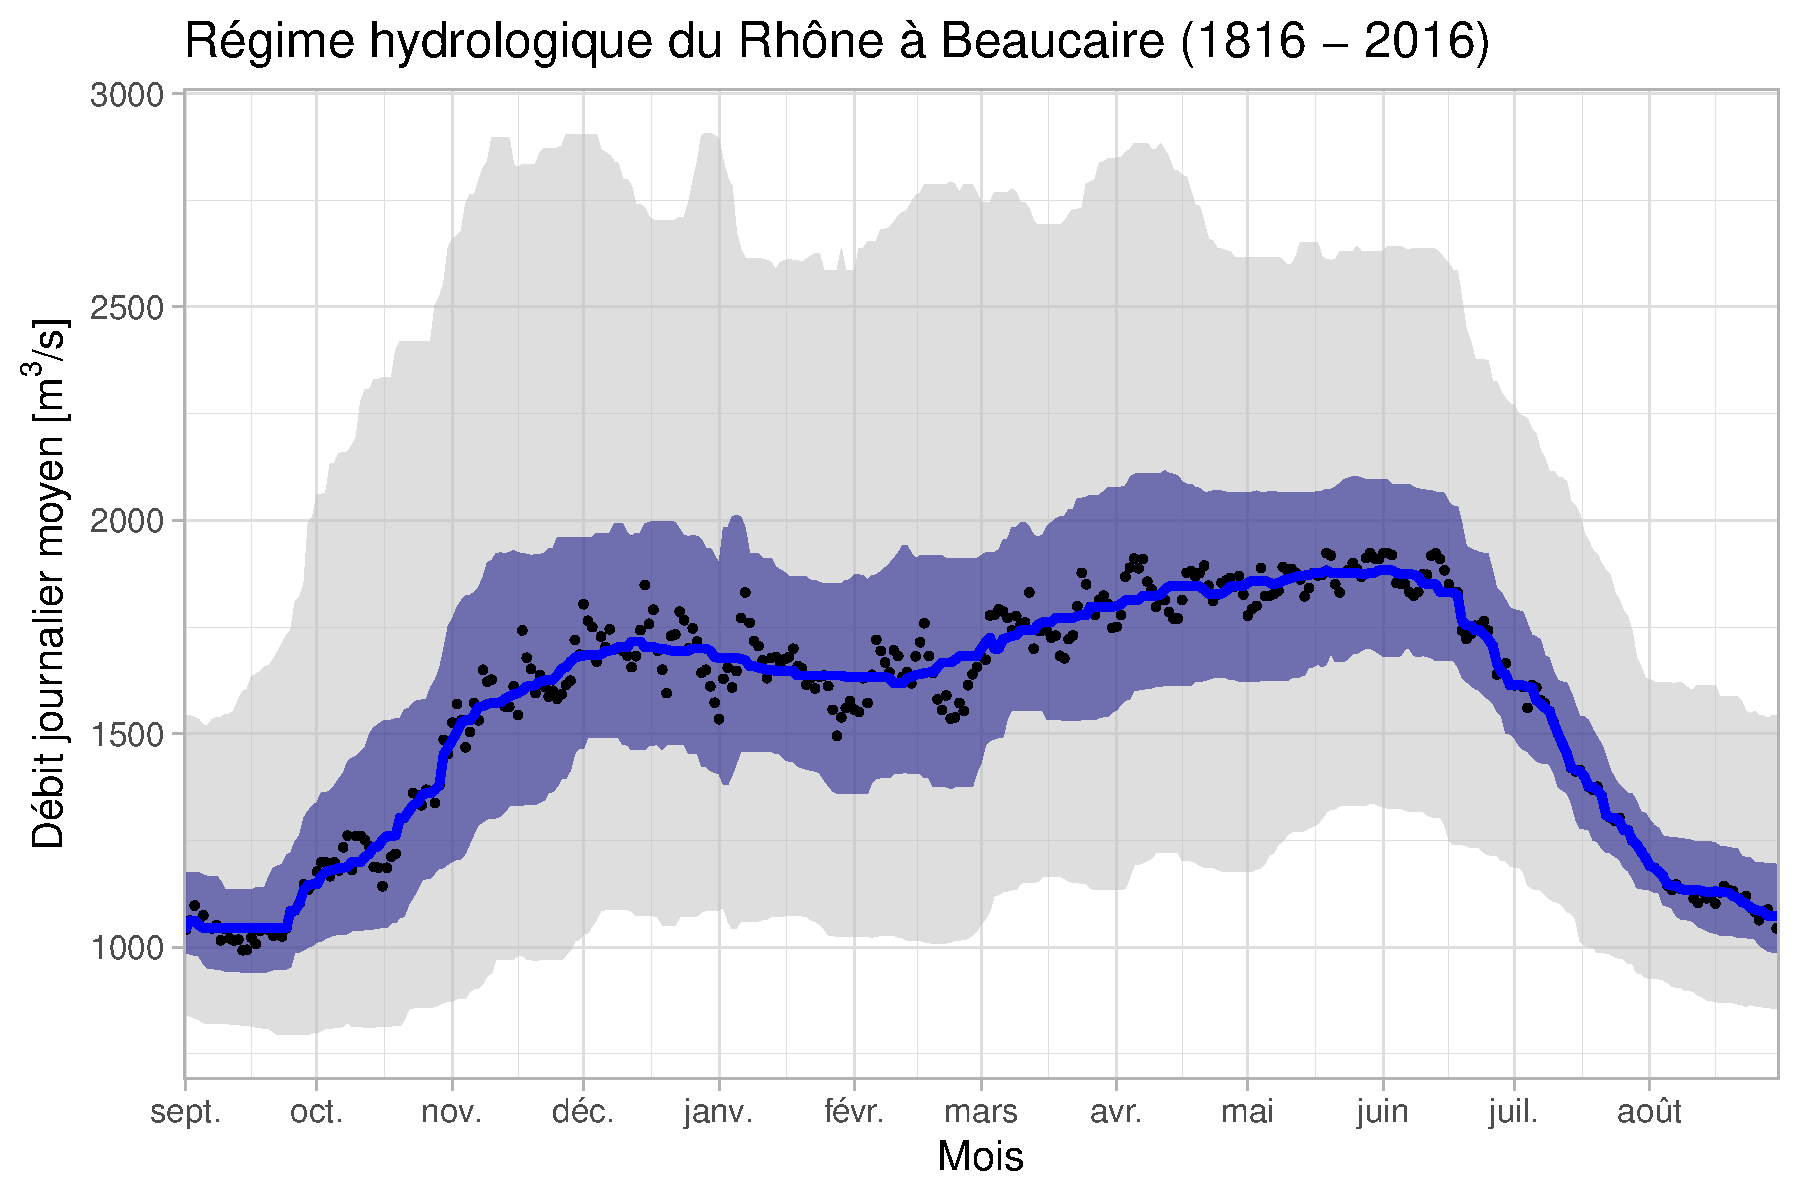
\includegraphics[width=.7\linewidth]{Figures/Regime.pdf}
        \caption{Débits moyens journaliers du Rhône à Beaucaire de 1816 à 2016 (points noirs). En bleu foncé, les quantiles 40 et 60\%, en gris les quantiles 20 et 80\%. La courbe bleue représente la médiane.}	
		\label{fig:Regime}
	\end{figure}


	
\FloatBarrier

	\subsection{Station hydrométrique du Rhône à Pont de Beaucaire (1816-1967)}
		
	\paragraph{} Le travail d'archive de \citet{pichard_les_1995} et \citet{pichard_hydro-climatology_2017} a permis de reconstituer une chronique continue d'observations de la hauteur d'eau du Rhône à Beaucaire à partir du 15 mai 1816 (tableau \ref{tab:MesuresPtBcr}). Ces relevés semble être les plus anciens qu'il soit possible de retrouver à Beaucaire (\cite{parde_regime_1925}; \cite{pichard_les_1995}). L'échelle limnimétrique fut installée au point kilométrique 267.7, sur le musoir de l'écluse du canal de Beaucaire à la mer dont les travaux furent achevés en 1811 (figure \ref{fig:CartoPt}). \citet{pichard_hauteurs_2013} souligne que « \textit{la longévité et la stabilité de cette échelle est (sic) évidemment exceptionnelle pour le bas Rhône. [...] La documentation chiffrée y est aussi précieuse et abondante qu'à Arles, mais cependant toujours aussi dispersée et accessible la plupart du temps par copie et non par les feuilles d'observations originales que les organismes gérants n'ont pas su conserver, en raison de transferts permanents d'attributions} ». Il faut noter que l'écluse du canal de Beaucaire fut remplacée entre 1914 et 1918 par une autre écluse débouchant plus à l'aval. Il semble cependant que le musoir que l'on observe de nos jours existait dès l'origine du canal et que l'échelle n'a subi aucun déplacement (\cite{pichard_hauteurs_2013}; \cite{bard_actualisation_2018}). 
	
	\begin{figure}[h]
	\centering
		\includegraphics[width=.8\linewidth]{Figures/CartoPt.pdf}
        \caption{(Gauche) Localisation de la station de Pont de Beaucaire (carte IGN 1950, source : www.geoportail.fr). (Droite) Échelle et limnigraphe CNR de Pont de Beaucaire en février 2020.}	
		\label{fig:CartoPt}
	\end{figure}

\FloatBarrier

	\subsubsection{Données disponibles}
	\paragraph{} Les relevés limnimétriques les plus anciens correspondaient probablement à une lecture d'échelle quotidienne en milieu de journée \citep{pichard_hauteurs_2013}. Après la crue généralisée de 1840 et la création du Service Spécial du Rhône, une norme de trois relevés par jour (à 7h, 12h et 17h) se met lentement en place (figure \ref{fig:RelevesPt}). L'application de cette norme n'est visible dans les données qu'à partir de 1887, et ce jusqu'à la fin de l'exploitation de la station.  L'année 1967 marque le début des travaux d'aménagement de l'ouvrage hydroélectrique de Vallabrègues et de son canal de dérivation, réalisés par la Compagnie Nationale du Rhône (CNR). Cette dérivation étant restituée à l'aval de la ville de Beaucaire, la station est déplacée 2 km plus à l'aval, environ 600 m à l'aval de la restitution des débits transitant par la centrale hydroélectrique. La nouvelle station, exploitée par la CNR à partir de 1970, sera alors appelée "Beaucaire Restitution". Le détail des relevés est indiqué dans le tableau \ref{tab:MesuresPtBcr}. Au final, ce sont plus de 200 ans de données limnimétriques continues qui sont disponibles à Beaucaire, et qui permettront une estimation du débit en continu sur cette période (chapitre 3 REF). 
	
	\begin{figure}[h]
          \centering
            \begin{subfigure}{0.49\linewidth}
            \centering
            	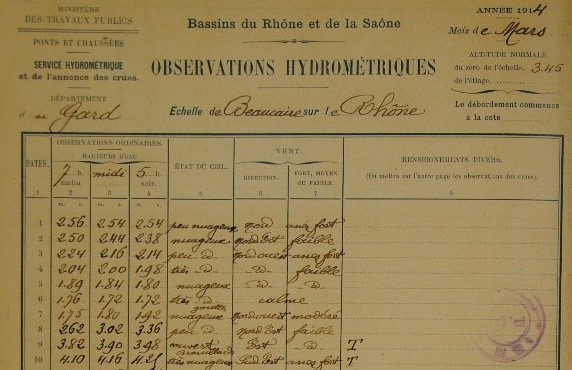
\includegraphics[width=1\linewidth]{Figures/TabObsBcrSmall.jpg}\hfill
            	\caption{}
            	\label{subfig:TabObsPt}
            \end{subfigure}
            \begin{subfigure}{0.49\linewidth}
            \centering
            	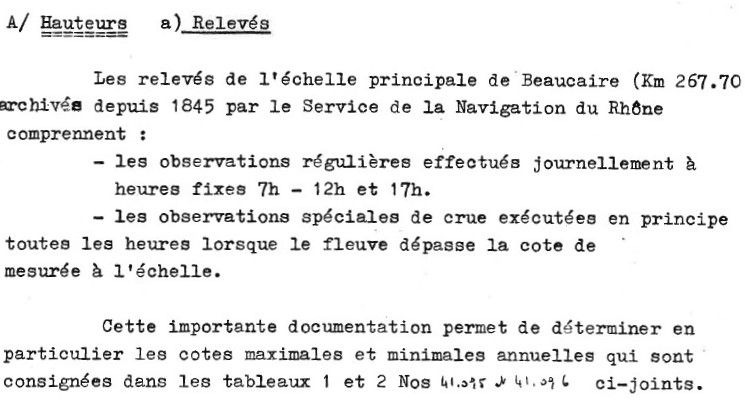
\includegraphics[width=1\linewidth]{Figures/RegleStationCNR}
            	\caption{}
           		\label{subfig:RegleCNR}
            \end{subfigure}
      \caption{(a) Feuille originale des relevés de hauteur d'eau à Beaucaire réalisés par le service spécial du Rhône en mars 1914. On remarque les trois relevés par jour ainsi que des précisions sur l'état du ciel ou le vent. (b) Règles d'exploitation de la station de Pont de Beaucaire, fiche station de la CNR. On remarque que des observations horaires sont effectuées au-delà d'une certaine cote dont la valeur n'est pas indiquée (Source : Archives CNR, 1962)}
	 \label{fig:RelevesPt}
	\end{figure}            
            
    
	\begin{table}[h]
	\centering
	\caption{Détail des relevés limnimétriques de la station de Pont de Beaucaire (PK 267.7)}
    \label{tab:MesuresPtBcr}
%	\resizebox{\columnwidth}{!}{%  
       \begin{tabular}{| m{2cm} | m{2.6cm}| m{2.2cm} | m{3cm} | m{2.7cm} | m{2.5cm} |} 
                \hline
               Période & Périodicité & Méthode & Origine & Zéro échelle [mNGF IGN69] & Commentaire \\
                \hline
                1816-1886 & 1 mesure/jour & Visuelle & 
                Service Spécial du Rhône & 3.37 & Probablement mesure à 12h \\
                \hline
                1887-1967 & 3 mesures/jour & Visuelle & 
                Service Spécial du Rhône & 3.37 & Relevés à 7h, 12h, 17h\\
                \hline
               1970-2020 & Horaire & Limnigraphe à flotteur puis LPN8 & 
                BD CNR & 0.06 &  \\
                \hline
		\end{tabular}
%		}
       \end{table}       
       
        
    \begin{figure}[h]
	\centering
		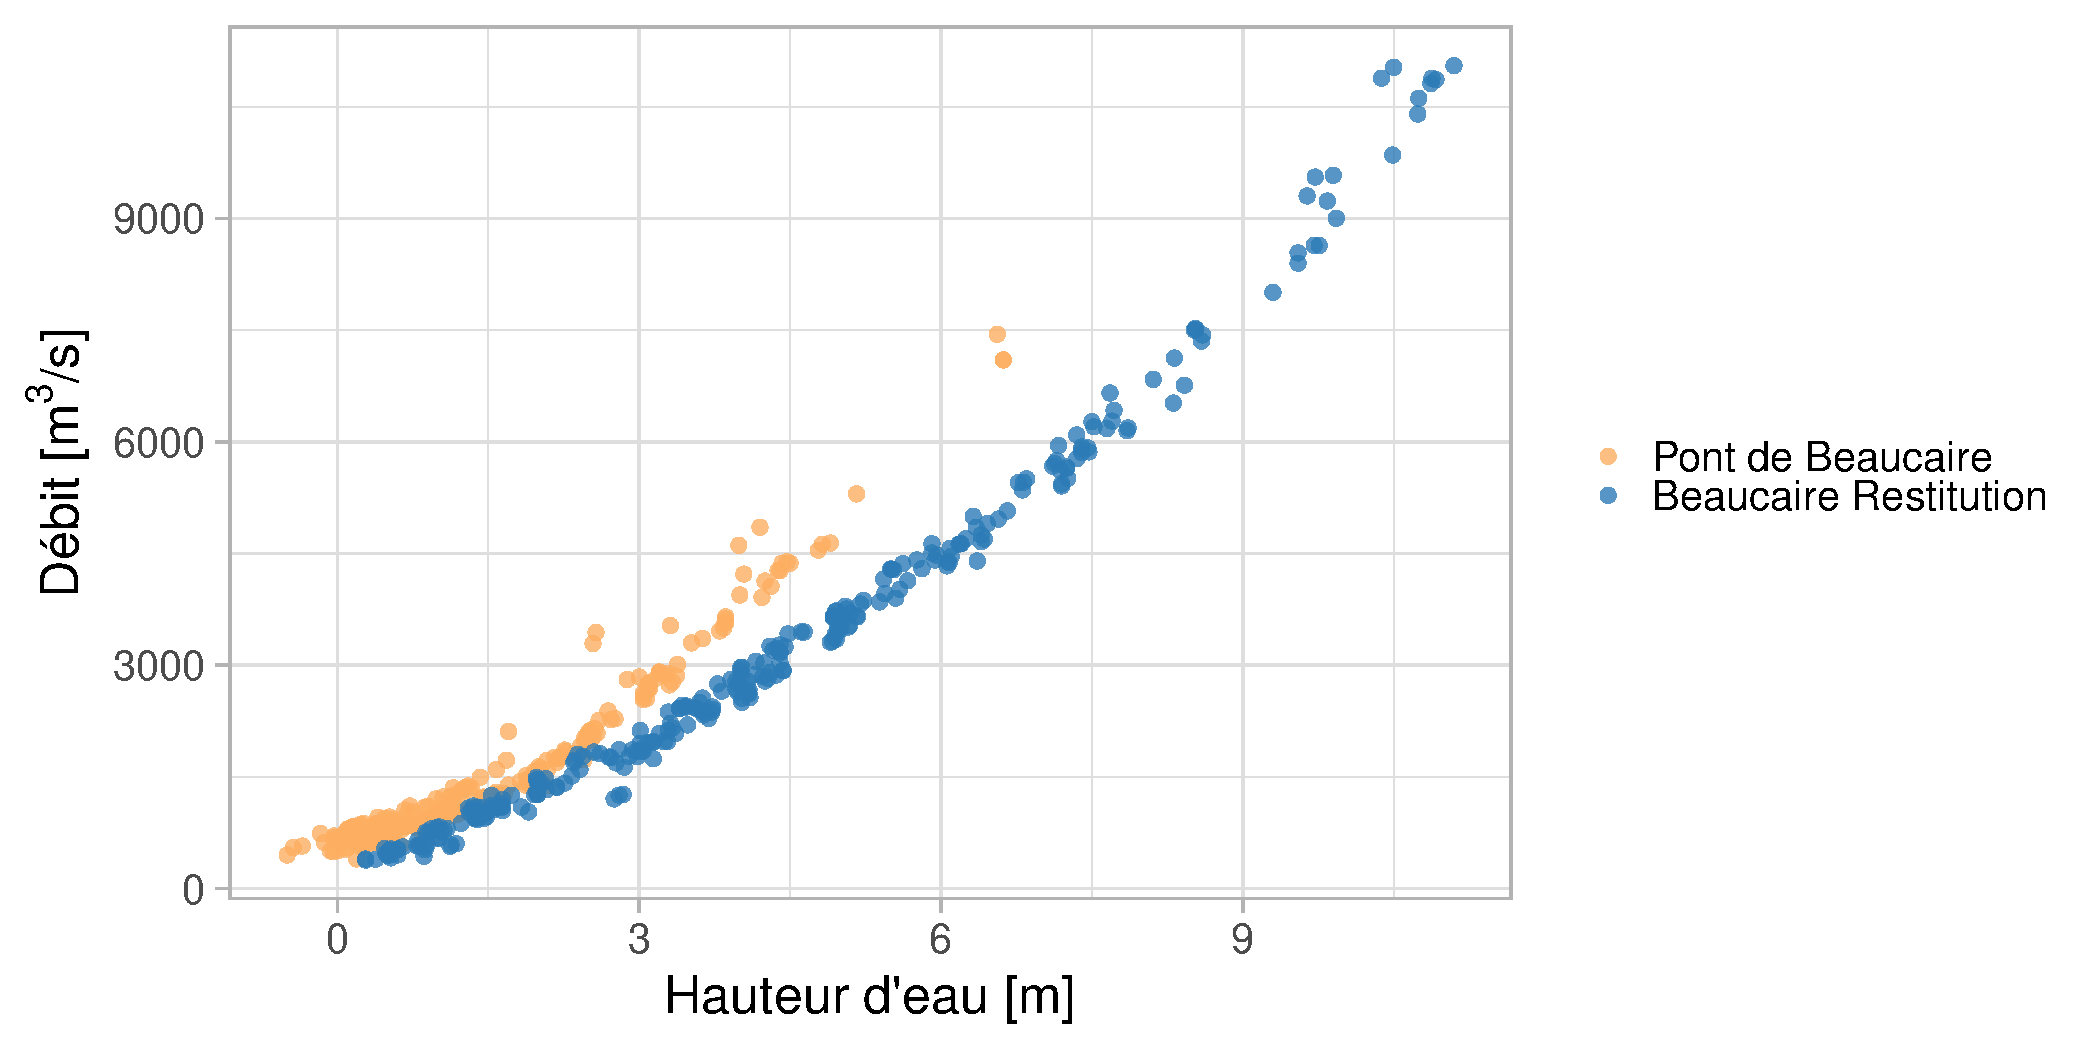
\includegraphics[width=.8\linewidth]{Figures/Jaus.pdf}
        \caption{Jaugeages à Pont de Beaucaire et Beaucaire Restitution de 1845 à 2020.}	
		\label{fig:JauAll}
	\end{figure}
       
    \paragraph{} Les jaugeages les plus anciens récupérés dans les archives départementales du Rhône datent de 1845 (figure \ref{fig:Jau1845}) alors que les mesures limnimétriques débutent en 1816. Il faut noter que les jaugeages étaient effectués à l'amont de la ville de Beaucaire, au PK 264.5, dans une zone plus stable et dépourvue d'îles indiquée sur la figure \ref{fig:CartoPt}. Quatre jaugeages des années 1845 et 1846 font exception à la règle et ont été effectués au droit de la station. Un total de 233 jaugeages est disponible à Pont de Beaucaire, couvrant la période 1845-1967 avec une fréquence peu homogène et des périodes non jaugées (notamment en période de guerre). Ils sont visibles sur la figure \ref{fig:JauAll}.
    
    \begin{figure}[h]
	\centering
		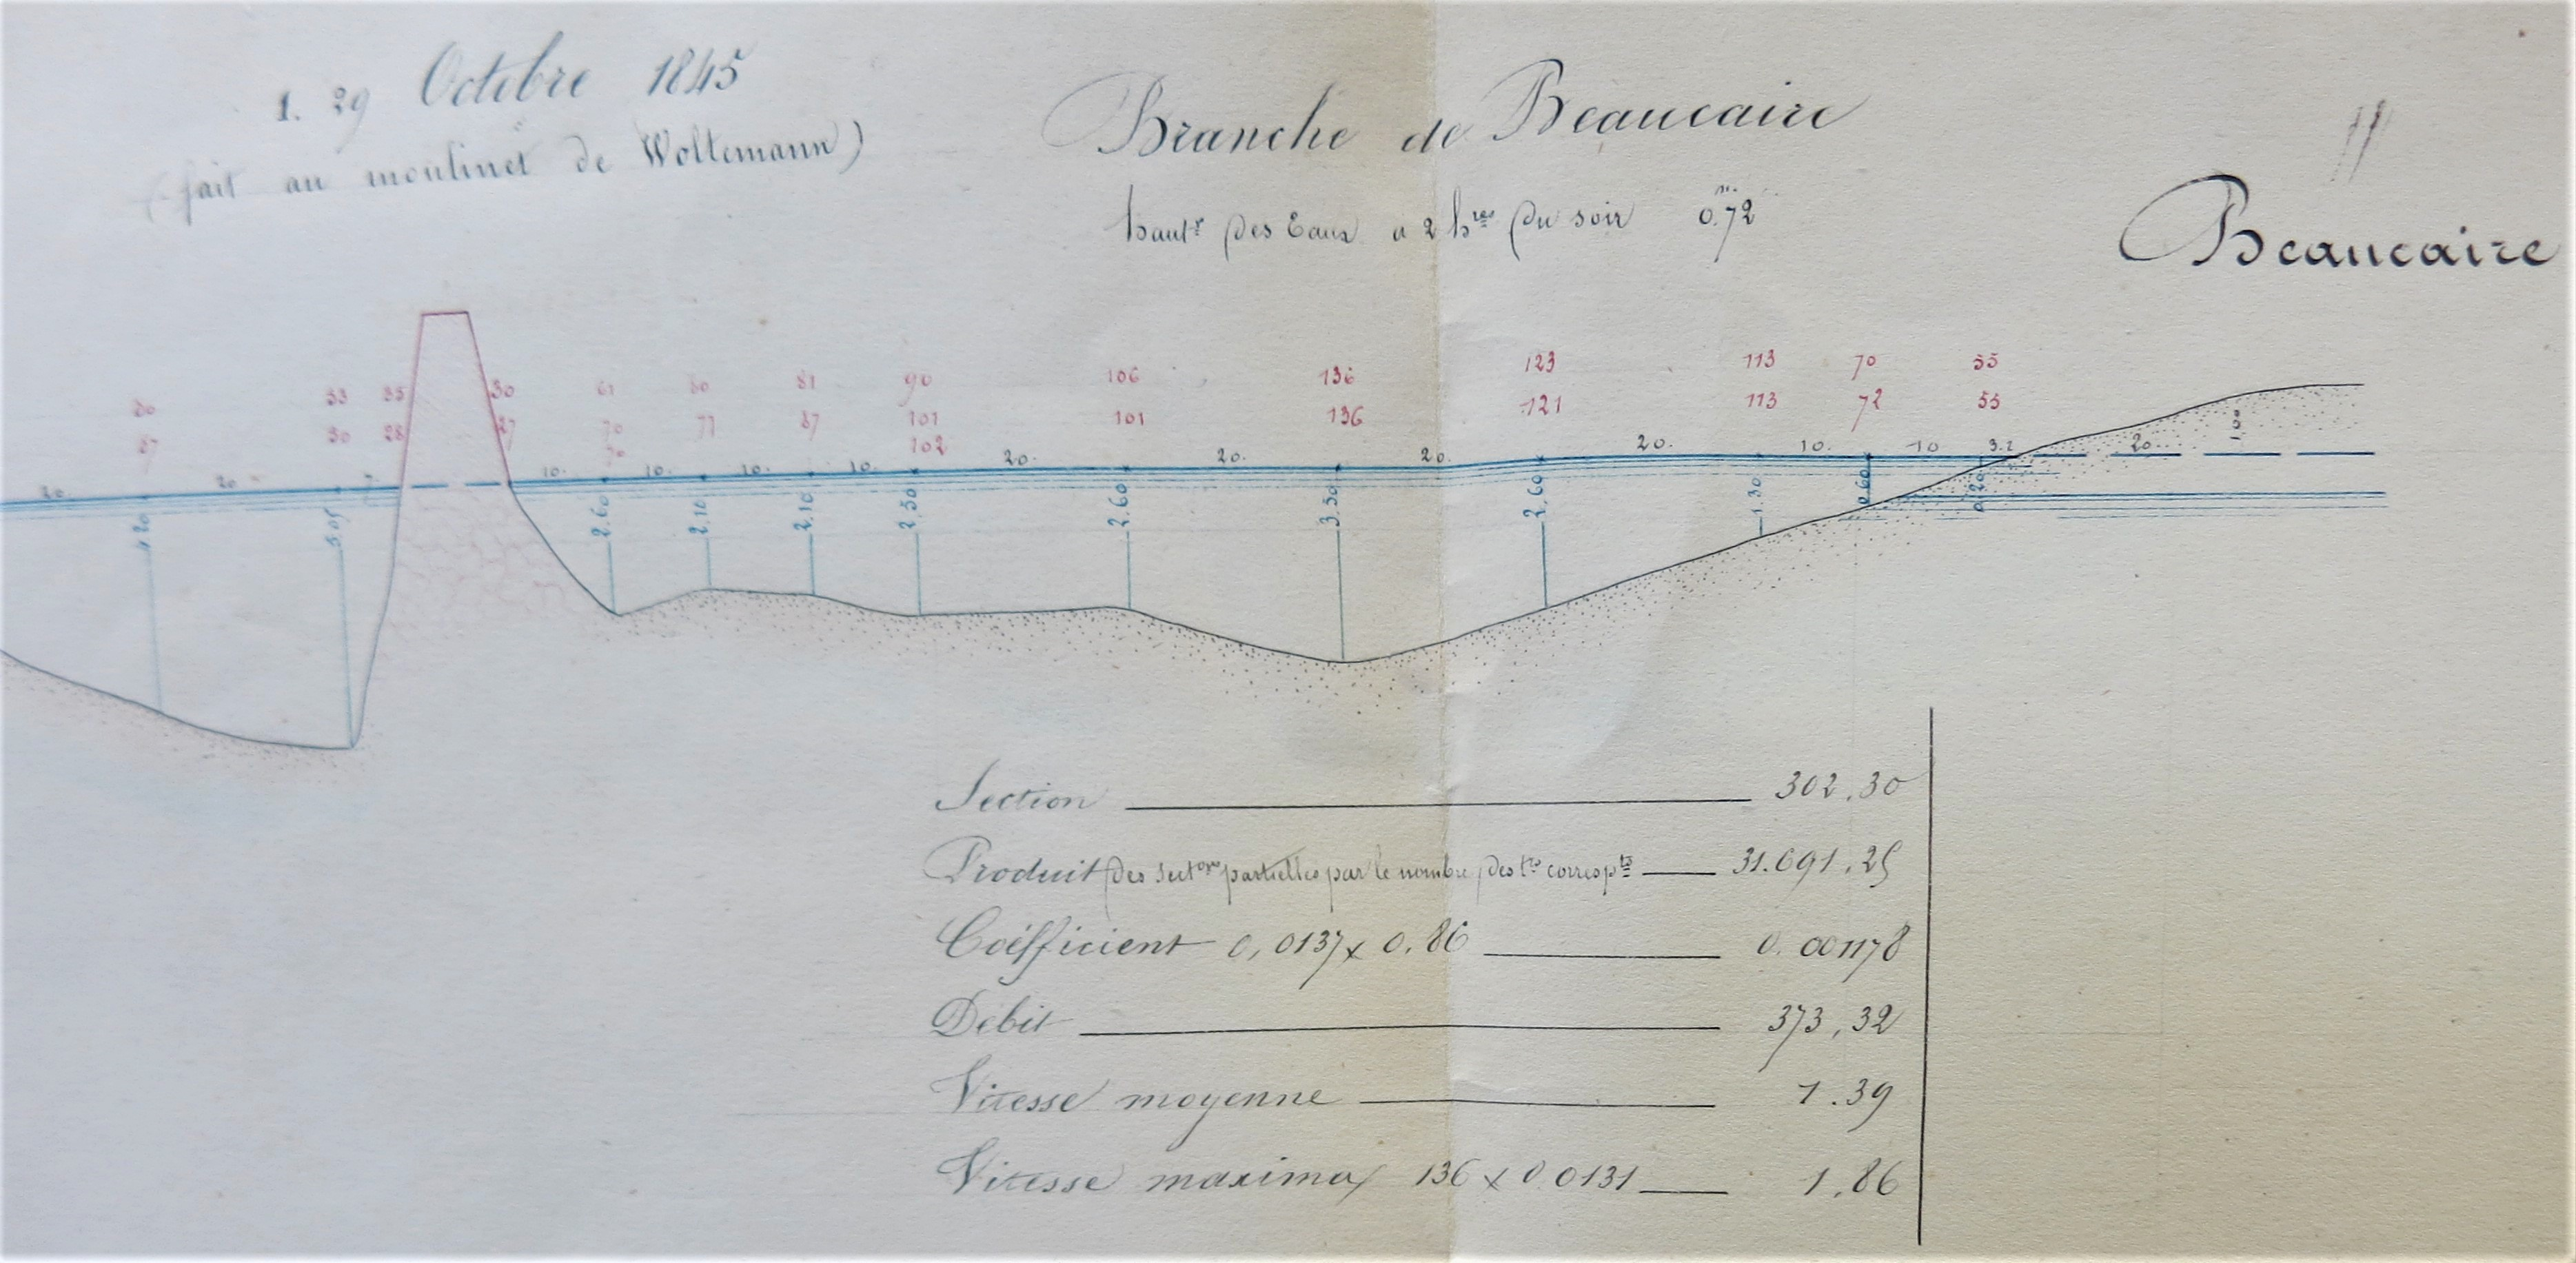
\includegraphics[width=.7\linewidth]{Figures/Jau1845.jpg}
        \caption{Jaugeage du 29 octobre 1845 au droit de la station de Pont de Beaucaire, réalisé au moulinet de Woltmann par le Service Spécial du Rhône. En bas à droite, le détail du calcul du débit. Les chiffres en rouge représentent le nombre de tours du moulinet, probablement moyennés sur une verticale.}	
		\label{fig:Jau1845}
	\end{figure}
    	
\FloatBarrier

	\subsubsection{Évolution de l'altitude du zéro de l'échelle}
    
    \paragraph{} Comme attesté par \citet{pichard_hauteurs_2013}, l'échelle limnimétrique de Pont de Beaucaire possède le rare avantage d'être restée à la même place depuis 1816, avec une altitude du zéro relativement stable dans l'histoire de la station. Malgré divers changements de référentiels altimétriques au cours du temps, le zéro semble n'avoir que très peu varié (tableau \ref{tab:zeroPt}). De la même manière que \citet{bard_actualisation_2018}, nous retiendrons la dernière mesure de la CNR qui semble être une valeur médiane de l'ensemble des valeurs connues : 3.37 m NGF IGN69. De plus, celle-ci est compatible avec les valeurs données lorsque la station était encore exploitée.

            \begin{table}[h]
                \centering
                \caption{Mesures de l'altitude du zéro de l'échelle à Pont de Beaucaire}
            	\label{tab:zeroPt}
                \begin{tabular}{| m{1.5cm} | m{3cm}| m{3cm} | m{2cm} |} 
                    \hline
                    Date & Altitude du zéro [m NGF IGN69] & Organisme \\
                    \hline
                    1959 &	3.375 &	CNR\\
                    \hline
                    1961 &	3.36 &	CNR\\
                    \hline
                    2010 &	3.38 &	Symadrem\\
                    \hline
                    2010 &	3.37 &	CNR\\
                    \hline
            \end{tabular}
        \end{table}


\FloatBarrier

		\subsubsection{Travaux et aménagements}
    	\label{subsubsec:TravauxPt}
    
    \paragraph{} La largeur de la section du Rhône au niveau de Beaucaire (ou du moins, la largeur du lit majeur) n'a que peu évolué dans l'histoire car elle se situe au niveau d'un resserrement entre deux collines rocheuses. Ce resserrement est bien visible sur les champs d'inondation de 1840 et 1856 (Figure \ref{Champ1856}). En revanche, à une échelle plus réduite, de nombreuses modifications morphologiques, d'origine naturelle ou anthropique ont pu affecter l'écoulement et modifier la relation hauteur/débit durant les deux siècles de relevés limnimétriques. Ces évolutions sont décrites dans les paragraphes suivants.
        
    \begin{figure}[h]
        \centering
        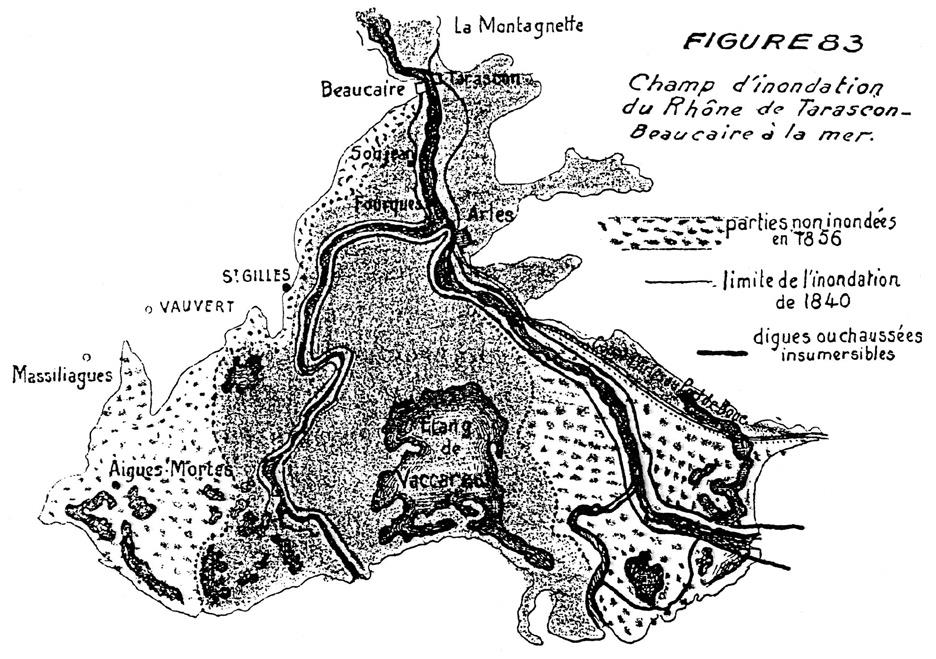
\includegraphics[width=.7\linewidth]{Figures/ChampInond1840-1856.jpg}
        \caption{Champ d'inondation du Rhône aval lors des crues de 1840 et 1856, d'après \citet{parde_regime_1925}}
        \label{Champ1856}
    \end{figure}
    

	\paragraph{} Le premier pont reliant Beaucaire à Tarascon date de 1829. Il s'agit d'un pont suspendu composé de 4 piles (d'après la carte d'état-major de 1840), situé environ 30 m à l'amont du pont actuel, soit environ 45 m à l'amont de l'échelle limnimétrique. Quelques années plus tard, en juillet 1852, était inauguré le viaduc de chemin de fer de Beaucaire. Il est situé environ 250 m à l'aval de la station. Par la suite, les seuls travaux significatifs qui ont eu lieu dans le secteur sont ceux de l'aménagement CNR de Vallabrègues, entre 1967 et 1970. Ils ont sonné la fin de l'utilisation de la station par la CNR, la mesure étant devenue non-significative de la totalité du débit du Rhône suite à la création du canal de dérivation de l'aménagement. On peut noter la construction du pont routier actuel, entre 1988 et 1990, 30 m à l'amont de l'ancien pont. 
        

        \paragraph{} À Beaucaire, depuis l'époque des plus anciennes cartes et des plus anciens récits jusqu'à aujourd'hui, des bancs de sable et îlots de diverses formes et dimensions ont séparé l'écoulement en deux bras plus ou moins distincts selon les périodes. De tout temps, mais pour des hauteurs d'eau différentes, les deux bras ont communiqué, un bras prenant le dessus sur l'autre au gré des événements morphogènes. Petit à petit, ces îlots ont été fixés par des digues afin de faciliter la navigation dans la zone, pour finalement arriver à la situation actuelle de deux bras bien distincts, comme en témoigne la carte d'\citet{armand_ii_1907} (figure \ref{fig:DigArmand}) qui décrit les différentes étapes de cette séparation :
        
         \begin{figure}[h]
            \centering
            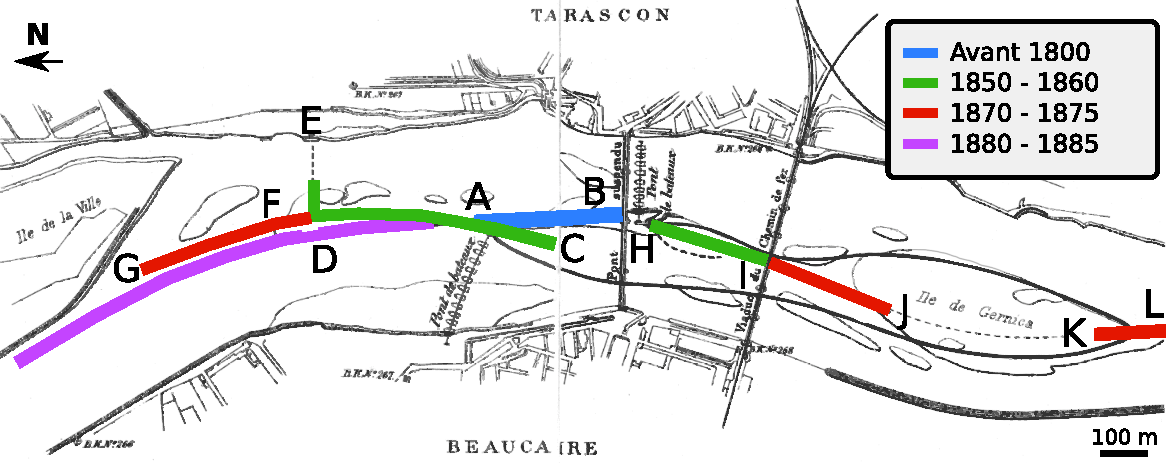
\includegraphics[width = 0.8\linewidth]{Figures/EditArmand.pdf}
            \caption{Carte de l'historique des digues de Beaucaire \citep{armand_ii_1907}}
            \label{fig:DigArmand}
        \end{figure}
        
        \begin{itemize}
            \item[$\bullet$] Digue divisoire (\textbf{AB}), antérieure à 1782
            \item[$\bullet$] Atterrissement (trait plein noir sur la carte) qui, dès 1826 se prolongeait jusqu'au point aval de l'île de Gernica. Il était probablement déjà présent au début du 19ème siècle.
            \item[$\bullet$] Érosion de l'île de la ville (à l'amont de Beaucaire) qui a modifié la répartition des débits entre les deux bras en faveur du bras de Tarascon. Pour maintenir la navigation dans le bras de Beaucaire, la digue \textbf{AB} fut prolongée à l'amont par une digue concave \textbf{CDF} en 1851 et par la suite, obstruction partielle du bras de Tarascon entre 1852 et 1855 \textbf{DE}. On peut constater cette érosion très rapide en faveur du bras de Tarascon sur les profils en travers de Goux (1850) (Figure \ref{fig:ProfGoux}). L'érosion de l'île de la ville peut être attribuée notamment à la crue catastrophique de 1840, possible déclencheur de ce phénomène.
            \item[$\bullet$] Forte érosion de l'atterrissement au niveau de \textbf{HI} du fait de l'écart de hauteur d'eau entre les deux bras pendant les crues. Une digue fut construite entre 1858 et 1859 pour pallier ce phénomène.
            \item[$\bullet$] Pour ces mêmes raisons, construction d'une digue en aval du viaduc de chemin de fer \textbf{IJ} en 1872-1875 ainsi que la digue \textbf{KL} à l'aval de l'île de Gernica, qui se prolonge actuellement sur 2 km vers l'aval.
            \item[$\bullet$] Prolongement de la digue concave \textbf{GF} autour de 1875
            \item[$\bullet$] Construction d'une nouvelle digue concave à l'amont de \textbf{GF} entre 1880 et 1884
        \end{itemize}

        \begin{figure}[h]
            \centering
            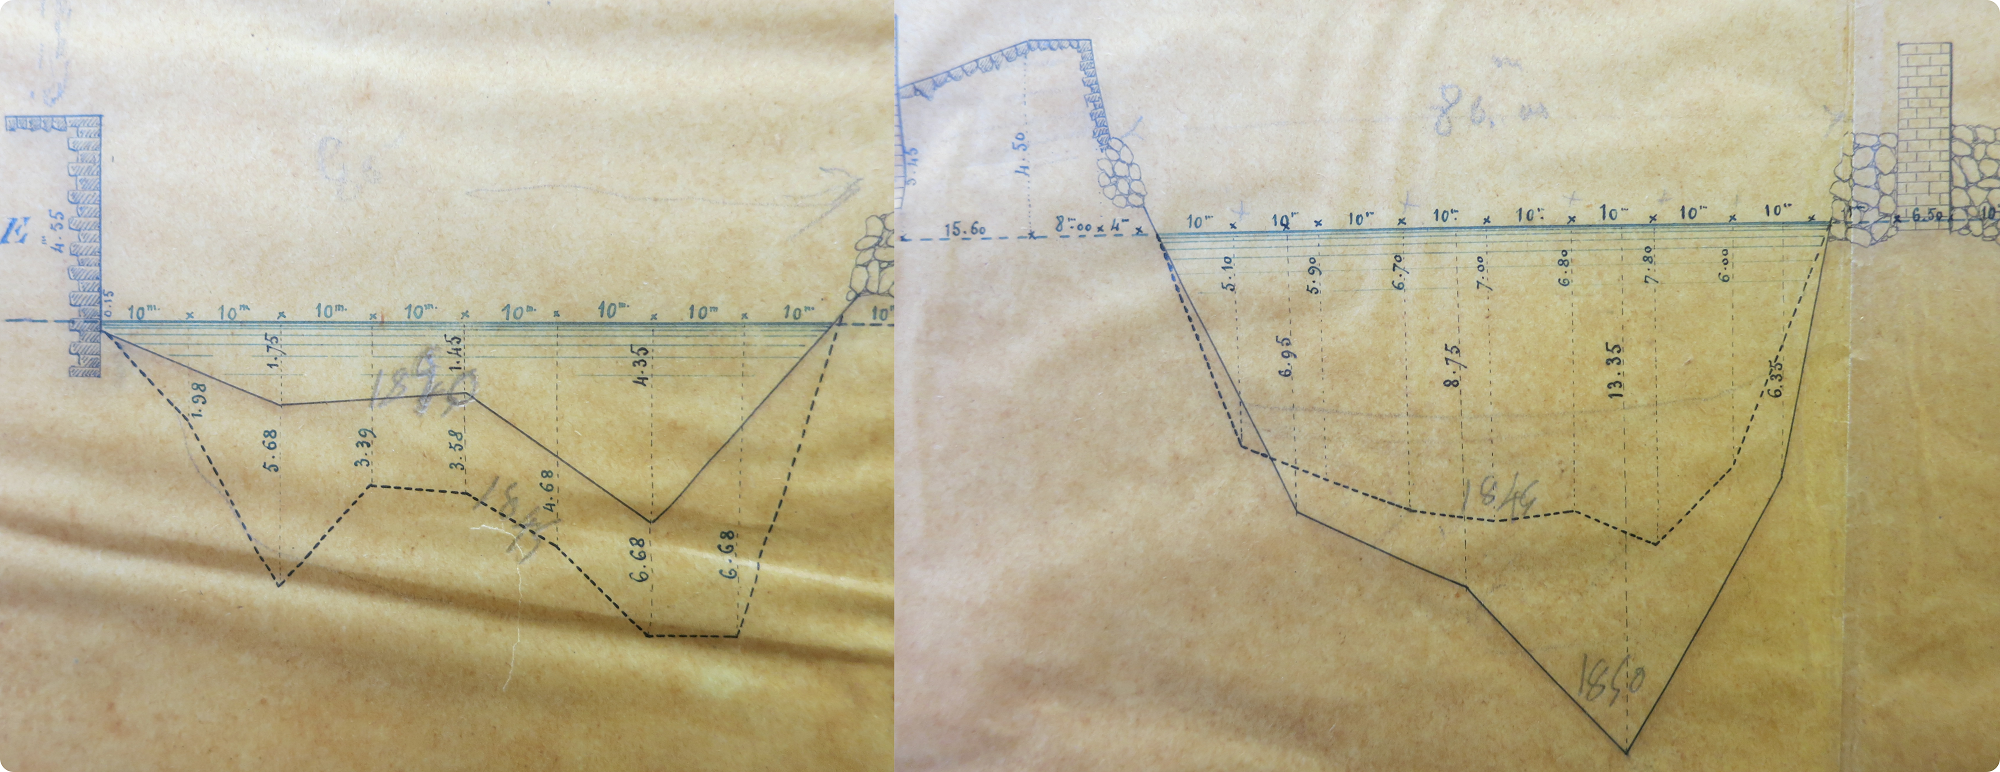
\includegraphics[width = 0.9\linewidth]{Figures/Goux4550.png}
            \caption{Portions de profil en travers au niveau du pont suspendu de Beaucaire. Il s'agit des bras de Beaucaire (gauche) et Tarascon (droite), en 1845 (pointillés) et 1850 (trait continu) \citep{goux_modification_1851}. On constate l'approfondissement du bras de Tarascon et le comblement du bras de Beaucaire.}
            \label{fig:ProfGoux}
        \end{figure}
%            
%        \begin{figure}[h]
%            \centering
%            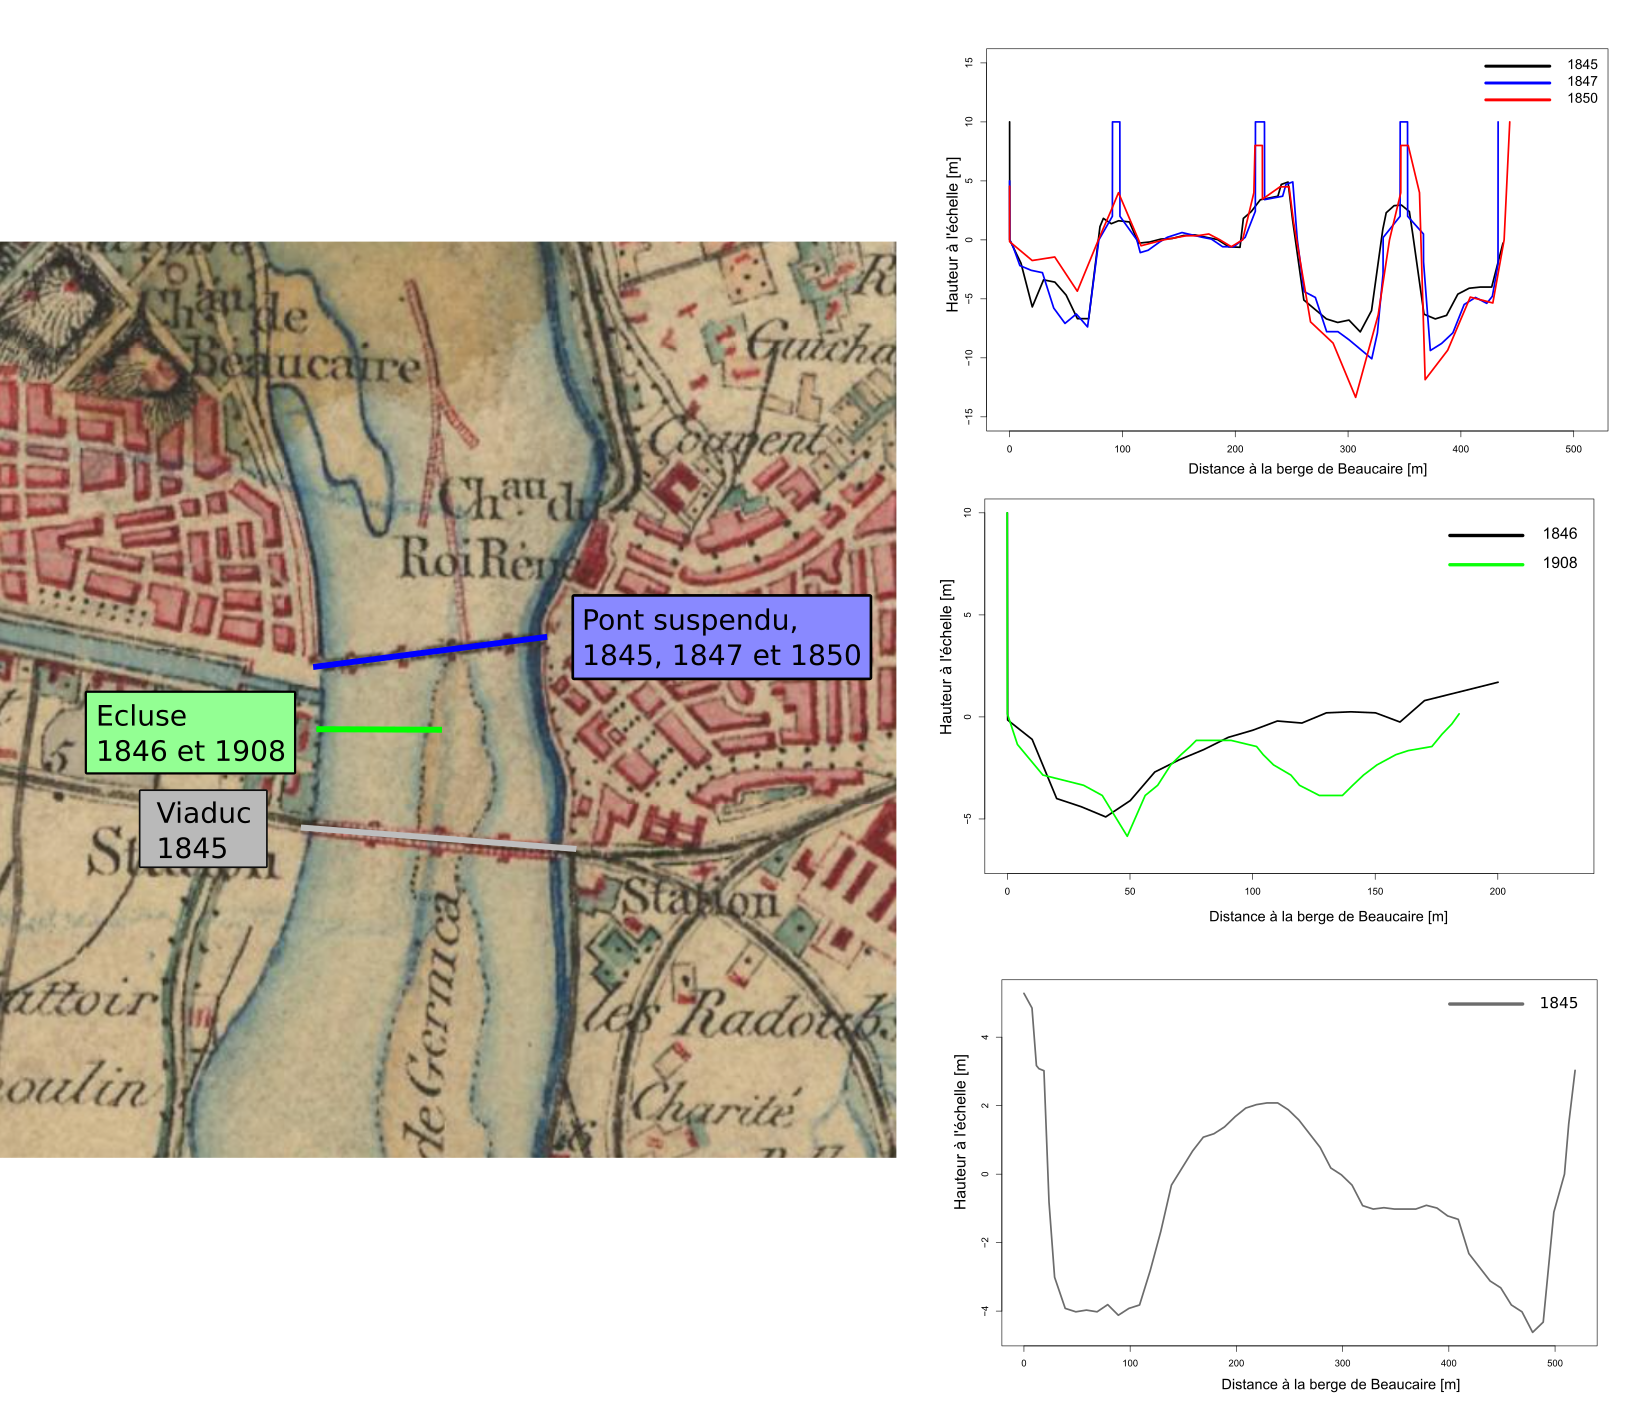
\includegraphics[width = 0.7\linewidth]{Figures/MapProfils.png}
%            \caption{Profils en travers du lit mineur du Rhône à Beaucaire au XIXème siècle}
%            \label{fig:Profils19eme}
%        \end{figure}
            
\FloatBarrier
        \paragraph{} Suite à la fixation des deux bras par les digues divisoires vers la fin du XIX\textsuperscript{ème} siècle, on peut supposer qu'il n'y a eu pratiquement aucun changement jusqu'au début des aménagements CNR de Vallabrègues (débutés en 1967 et mis en service en 1970), comme en témoignent les photos aériennes du portail "Remonter le temps" de l'IGN, de 1936 à 1947 (Figure \ref{fig:AerialBcr}). Ainsi, l'isolement quasi-total du bras de Tarascon au profit du bras de Beaucaire est finalisé en 1884 et a connu de nombreuses phases d'aménagement débutant vers la fin du 18\textsuperscript{ème} siècle. Il est probable qu'à l'époque ancienne, tout comme aujourd'hui, les deux bras communiquaient à haut débit, certainement aux alentours de 6 m à l'échelle à l'époque de la finalisation des digues, et à des hauteurs moindres auparavant. Certaines sources signalent par exemple qu'il était ponctuellement possible de traverser en bateau d'un bras à l'autre au niveau de la ville entre 1858 et 1872. Le bras de Beaucaire a sans doute été prépondérant sur le bras de Tarascon sur la majeure partie de l'histoire de la station, excepté durant la période 1840-1850, comme en témoignent les profils en travers de \citet{goux_modification_1851} (Figure \ref{fig:ProfGoux}).
    
        \begin{figure}[h]
            \centering
        	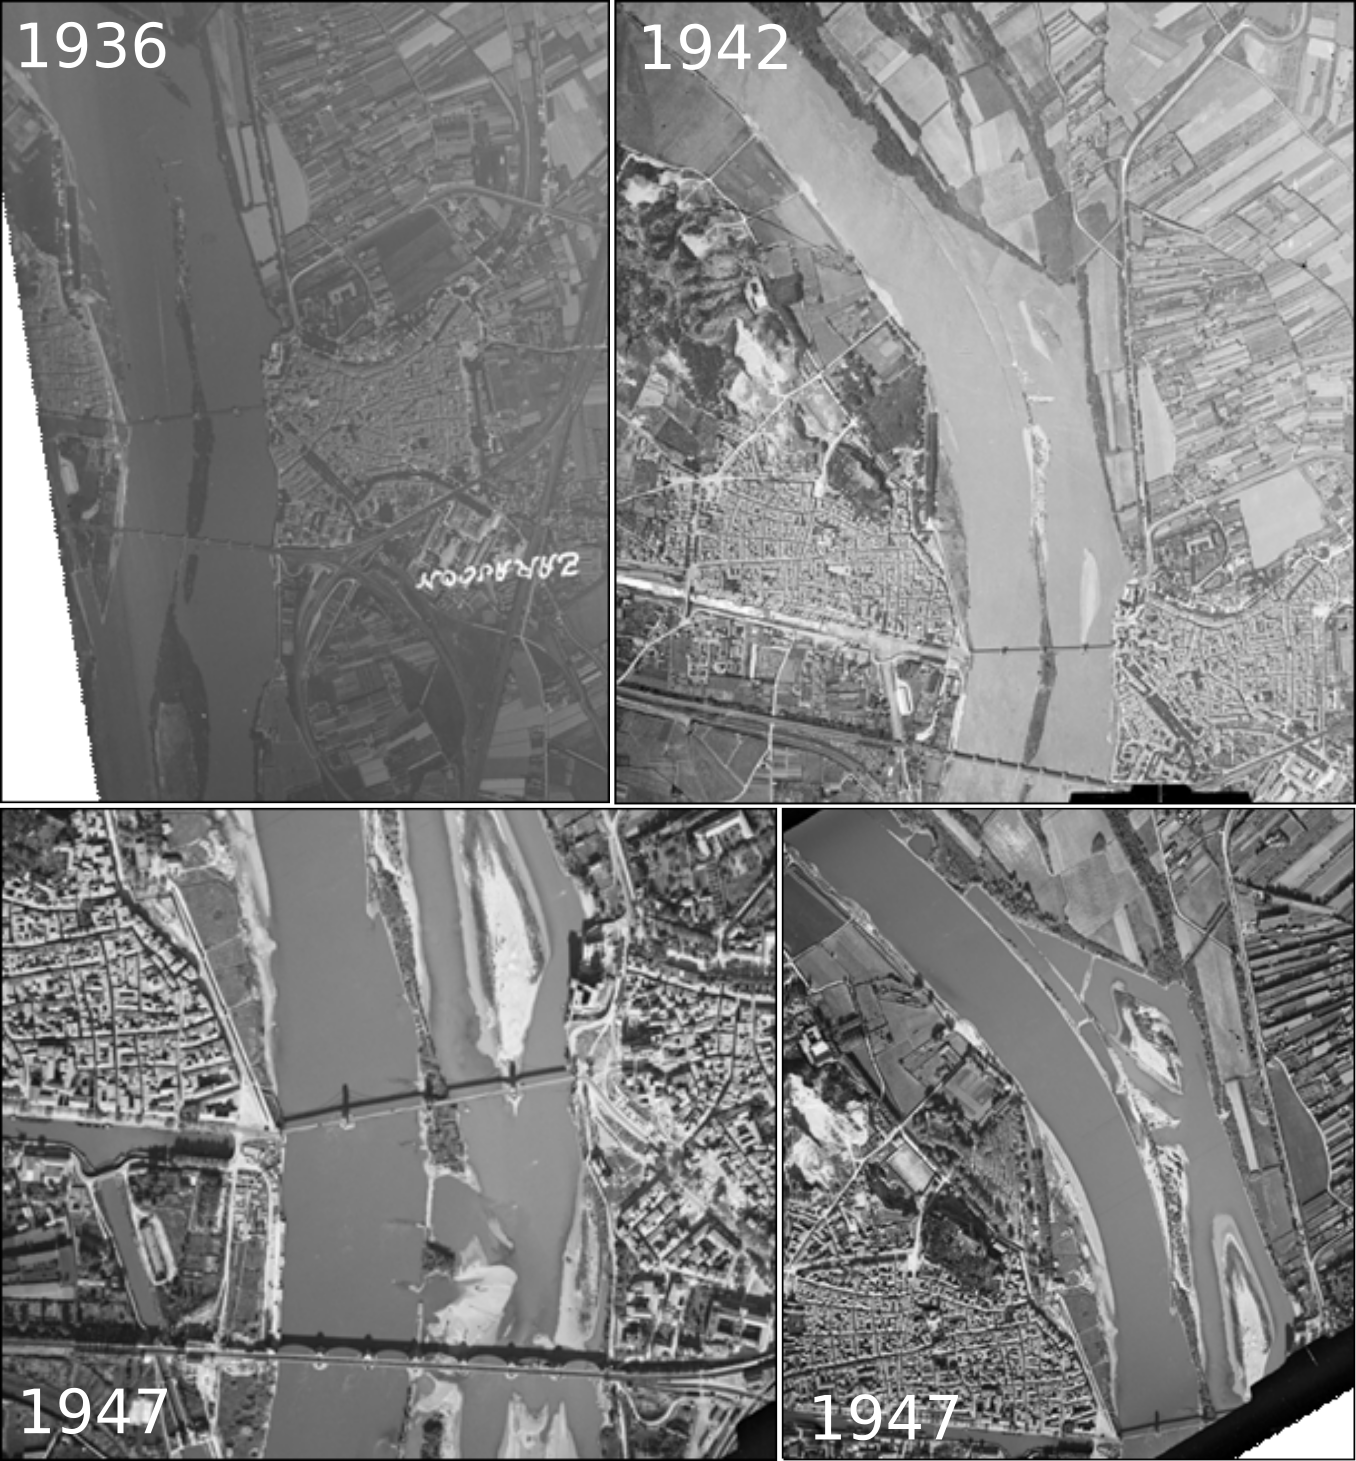
\includegraphics[width = 0.7\linewidth]{Figures/AerialBcr.png}
            \caption{Images aériennes du Rhône à Beaucaire entre 1936 et 1947 (source : www.géoportail.gouv.fr). On remarque la présence des digues sur les 4 images, particulièrement en 1947 pour des débits très faibles.}
            \label{fig:AerialBcr}
        \end{figure}
    
		\paragraph{} Au cours des décennies 1860 et 1870, les travaux d'aménagement en lit mineur imaginés par l'ingénieur Girardon sont lancés. Ils permettront de favoriser la navigation fluviale en fixant les berges par l'installation d'épis noyés transversaux sur une grande partie du linéaire du Rhône français. Des épis ont été installés à l'amont et à l'aval de Beaucaire et ont probablement influencé la relation hauteur/débit au droit de la station.
    
		\paragraph{} Les désordres du Rhône à l'aval de Beaucaire étant réguliers avant son endiguement, on imagine que la création des digues a coïncidé avec l'installation des populations dans le secteur, comme attesté par \citet{surell_memoire_1847} : "\textit{Si l'on considère que l'existence de la plaine est presque inévitablement liée à celle des chaussées, on doit croire que celles-ci sont contemporaines de la civilisation même du pays, et qu'elles ont dû occuper, depuis longtemps, les soins de la population}" (les digues étaient fréquemment appelées chaussées dans l'époque ancienne, car elles faisaient également office de voies de circulation). \citet{mejean_etude_2017}, cite l'ingénieur Girard, qui, en 1857, affirme que : "\textit{la construction des premières chaussées entre Beaucaire et Sylvéréal (Camargue) date de l'époque romaine. L'initiative personnelle des propriétaires a ensuite contribué à dresser un système de protection où chacun établissait une levée de terre pour se protéger des invasions du Rhône. La plupart de ces chaussées étaient établies sur les bourrelets alluviaux, car ils présentaient l'avantage d'être déjà surélevés par rapport aux terres voisines. Les chaussées ne présentaient pas une ligne continue de défense, les protections s'établissant autour de quelques grandes propriétés.}" Par la suite, plusieurs grandes phases d'aménagement des digues de protection se sont succédées. Avant le XVI\textsuperscript{ème} siècle, les aménagements étaient discontinus mais deviennent plus organisés avec l'essor de l'agriculture dans les plaines alluviales. Au début du XIX\textsuperscript{ème} siècle, un endiguement continu de Beaucaire à la mer est installé grâce à l'harmonisation des nombreuses associations ou "syndicats des digues", jusqu'alors "\textit{aussi multiples que rivales}" \citep{pichard_sept_2014}. Cet endiguement protège les populations pour les crues courantes et jusqu'à la décennale. Au niveau de Beaucaire, la digue de la Montagnette existant depuis le XV\textsuperscript{ème} siècle connut de nombreuses avaries en 1840, 1841, 1843. Des travaux de rehaussement furent effectués en 1843 ainsi qu'en 1883. La digue du chemin de fer (de Tarascon à Arles en rive gauche) vint remplacer en 1846 les digues historiques du Trébon, souvent rompues dans l'histoire. La digue du Trébon était élevée à 6.5 ou 7 m au-dessus de l'étiage. La digue du chemin de fer est élevée à 2.10 m au-dessus des plus hautes eaux connues à l'époque (1843). Lors de la rupture de la digue de la Montagnette en 1856, Tarascon était enfermée entre Montagnette et le remblai du chemin de fer, l'eau était ainsi restée dans les plaines pendant plusieurs semaines. Ces digues principales furent complétées par des aménagement au sein des villes de Tarascon et Beaucaire entre 1860 et 1866. La "banquette de Beaucaire", constituée d'un mur maçonné construit en 1840 du rocher du château à la chaussée du chemin de fer, fut rehaussée après 1856, puis en 1862 et 1863, environ 2 m au-dessus du niveau atteint en 1856. Il en va de même pour les quais de Tarascon et de la digue de la Montagnette, rehaussés en 1860 à 1.5 m au-dessus du niveau de 1856.
		
		\paragraph{} Ces nombreuses protections érigées au cours du XIX\textsuperscript{ème} siècle ont permis de contenir les crues courantes, puis des crues plus importantes grâce aux aménagements postérieurs aux inondations de 1840 et 1856 qui furent à l'origine d'une prise de conscience illustrée par la création du Service Spécial du Rhône par les Ponts et Chaussées. Depuis cette époque, les systèmes de protection n'ont que peu évolué et la crue de 2003 a ravivé les inquiétudes quant au risque de brèches, comme en témoigne cet extrait du rapport du \citet{symadrem_programme_2012} (Syndicat Mixte Interrégional d'Aménagement des Digues du Delta du Rhône et de la Mer) : "\textit{Le système actuel de protection contre les crues du Rhône a été réalisé après les grandes crues de 1840 et 1856. Il est ancien et présente une exposition très forte au risque de brèches. Dans l'état actuel, on estime que que le risque de formation de brèches, confirmé par les crues de 1993, 1994, 2002 et 2003, est quasi-certain à certain}". Depuis la crue de 2003, un programme de sécurisation a été réalisé, prévoyant notamment la réalisation de digues résistantes à la surverse et à la formation de brèches \citep{symadrem_programme_2012}.    
		
	
\FloatBarrier
	\subsection{Station hydrométrique du Rhône à Beaucaire Restitution (1970-aujourd'hui)}
	
	\subsubsection{Données disponibles}

	\paragraph{} La station de Beaucaire Restitution (PK 269.6) a pris le relais sur la station de Pont de Beaucaire suite aux travaux de l'aménagement hydroélectrique de Vallabrègues, et de l'installation d'un chenal de dérivation restituant une partie du débit à l'aval de la ville de Beaucaire. La nouvelle station fut alors installée 2 km plus à l'aval, environ 600 m à l'aval de la restitution des débits transitant par la centrale hydroélectrique CNR de façon à mesurer la totalité du débit (figure \ref{fig:CartoRes}). Durant les travaux, de 1967 à 1970, les débits de la Durance ayant été dérivés vers l'étang de Berre, les relevés des deux stations sont considérés comme manquants. La station de Beaucaire Restitution demeure au même emplacement depuis sa mise en service en 1970. Elle est équipée dès sa création de capteurs automatiques réalisant des relevés au pas de temps infra-horaire. L'ensemble de ces relevés, ainsi que les jaugeages réalisés à la station, sont disponibles au sein des bases de données de la CNR.
		
	\begin{figure}[h]
	\centering
		\includegraphics[width=.8\linewidth]{Figures/RestitCartoPh.png}
        \caption{Gauche : Localisation de la station de Beaucaire Restitution (carte IGN Scan25, source : www.geoportail.fr). Droite : échelle limnimétrique de Beaucaire Restitution en février 2020.}	
		\label{fig:CartoRes}
	\end{figure}
	
	
		\subsubsection{Travaux et aménagements}

	\paragraph{} La section du Rhône au niveau de la station de Beaucaire Restitution a connu de nombreux dragages des matériaux du fond du lit suite à la construction de l'aménagement de Vallabrègues, durant les 5 années après la mise en service du système en 1970, ainsi qu'entre 1998 et 2000, pendant la construction du nouveau pont routier reliant Tarascon à Beaucaire. En dehors de ces interventions, le profil au droit de la station est stable, comme en témoignent les profils en travers du lit mineur au droit de la station (figure \ref{fig:ProfilsRestit}).
	
	\begin{figure}[h]
	\centering
		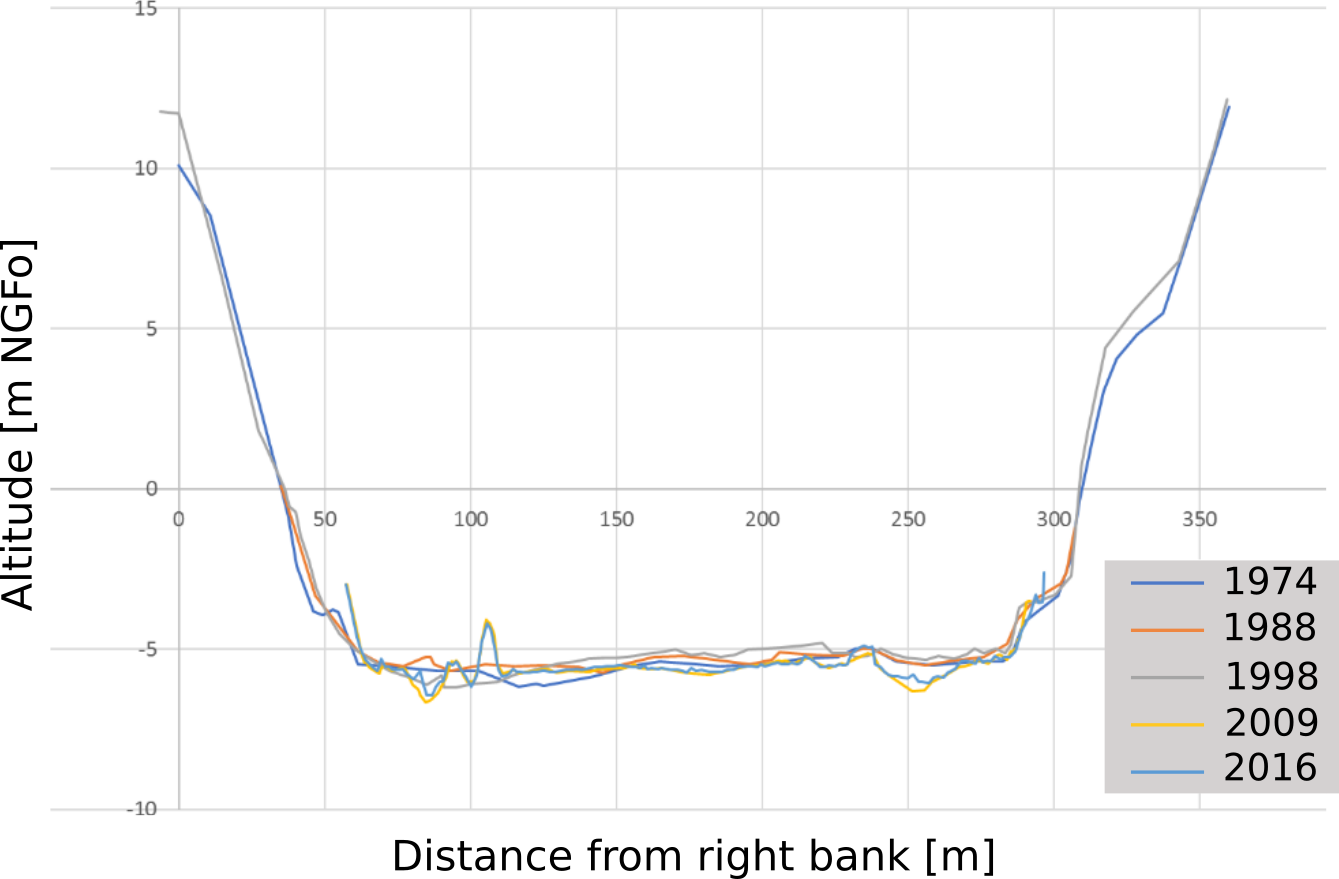
\includegraphics[width=.6\linewidth]{Figures/ProfilsBardRestit.png}
        \caption{Profils en travers du Rhône à la station de Beaucaire Restitution réalisés par la CNR entre 1974 et 2016. Adapté de \citet{bard_actualisation_2018}. On passe de l'altitude NGF ortho (ou Lallemand) à l'altitude NGF IGN69 en ajoutant 3 cm.}	
		\label{fig:ProfilsRestit}
	\end{figure}
	
\FloatBarrier


\subsection{Évolution du temps de propagation des crues}

	\paragraph{} Les aménagements en lit mineur du Rhône français, débutés dès la seconde moitié du XIX\textsuperscript{ème} siècle, ont eu des conséquences directes sur la géométrie du chenal. Rapidement, la largeur du lit mineur et la ligne d'eau ont été impactées (\cite{gaydou_schema_2013}; \cite{piegay_observatoire_2022}). Une conséquence de ces aménagements pourrait être la modification de la dynamique d'écoulement des crues sur le continuum fluvial. On peut en effet se demander si la transition d'un style fluvial naturel et complexe vers un chenal unique et quasiment rectiligne (figure \ref{fig:CartesChenal}) n'aurait pour conséquence de modifier la vitesse de propagation des événements de crue, mais également d'impacter le laminage des crues le long de la moyenne et basse vallée du Rhône. Ces modifications morphologiques pouvant impacter la stationnarité des débits, et donc l'analyse fréquentielle des crues, leurs conséquences sont étudiées dans cette section.
	
	\begin{figure}[h]
		\centering
		\begin{subfigure}{0.4\linewidth}
			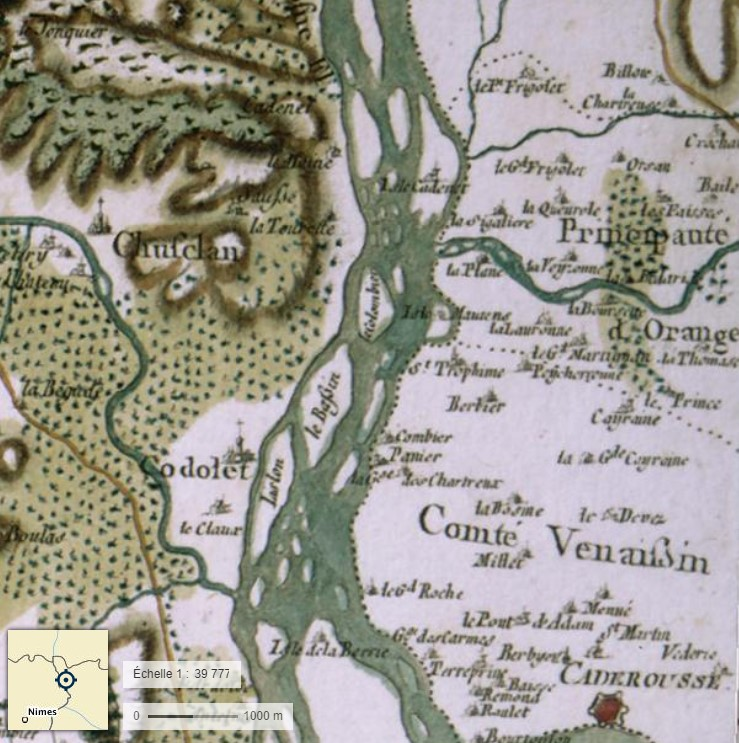
\includegraphics[width=\linewidth]{Figures/CassiniOrange.jpg}
		\end{subfigure}
		\begin{subfigure}{0.4\linewidth}
			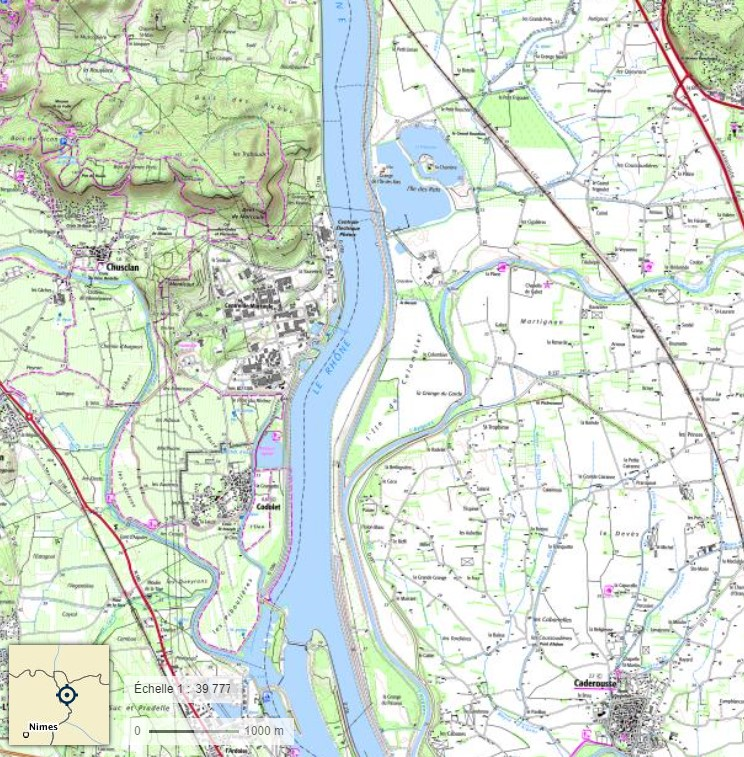
\includegraphics[width=\linewidth]{Figures/IGNOrange.jpg}
		\end{subfigure}
		\caption{Cartes du Rhône au niveau de la ville d'Orange (environ 50 km à l'amont de Beaucaire). A gauche, la carte de Cassini datant du XVIII\textsuperscript{ème} siècle présente un chenal en tresses. A droite, la carte IGN actuelle présente un chenal unique et contraint. (source : \url{geoportail.gouv.fr})}
		\label{fig:CartesChenal}
	\end{figure}
	
	\paragraph{} Dans le but d'étudier l'impact au cours du temps des aménagements en lit mineur sur le temps de propagation des crues, il est possible d'analyser le délai entre le passage du pic de crue à l'amont et à l'aval du linéaire aménagé. "\textit{Les aménagements Girardon […] conçus et mis en place entre 1880 et 1920 […] sont présents depuis le pont de Rochefort en amont [environ 80 km à l'aval du lac Léman], jusqu'à la mer. Ils sont moins nombreux en amont de Lyon, où ils se limitent à une digue longitudinale basse et des épis}" \citep{gaydou_schema_2013}. Suite à ce constat, il est décidé de limiter l'analyse au linéaire entre Lyon et Beaucaire, considérant que les aménagements présents à l'amont de Lyon, par leur forme différente et leur moindre présence, n'ont eu que peu d'influence sur la dynamique des crues à Beaucaire.
	
	\paragraph{} Les aménagements en lit mineur du Rhône ont été conduits en plusieurs phases au cours des deux derniers siècles. Tout d'abord, la construction des premières digues pour l'amélioration de la navigation au milieu du XIX\textsuperscript{ème} siècle (section \ref{subsubsec:TravauxPt}). Ensuite, des travaux de plus grande ampleur organisés par l'ingénieur Girardon ont été réalisés sur l'ensemble du linéaire français entre 1880 et 1920. Ces travaux consistent notamment en l'installation d'épis et de casiers immergés qui concentrent l'écoulement vers le centre du chenal (figure \ref{subfig:Girardon}). Ce n'est ensuite qu'à partir de 1948 que de nouveaux travaux sont réalisés. Il s'agit de l'installation de 18 ouvrages hydroélectriques effectuée par la CNR sur l'ensemble du cours du Rhône français jusqu'en 1989. Ces aménagements sont pour la plupart construits sur un même schéma, à savoir l'installation d'un canal de dérivation qui court-circuite le chenal originel du Rhône, alors appelé "Vieux-Rhône" (figure \ref{subfig:SchemaCNR}). Ce sont donc trois grandes phases d'aménagement qui ont eu lieu depuis le début du XIX\textsuperscript{ème} siècle et qui ont indéniablement eu des conséquences sur la dynamique des écoulements. 
	
	\begin{figure}[h!]
		\centering
		\begin{subfigure}{0.7\linewidth}
		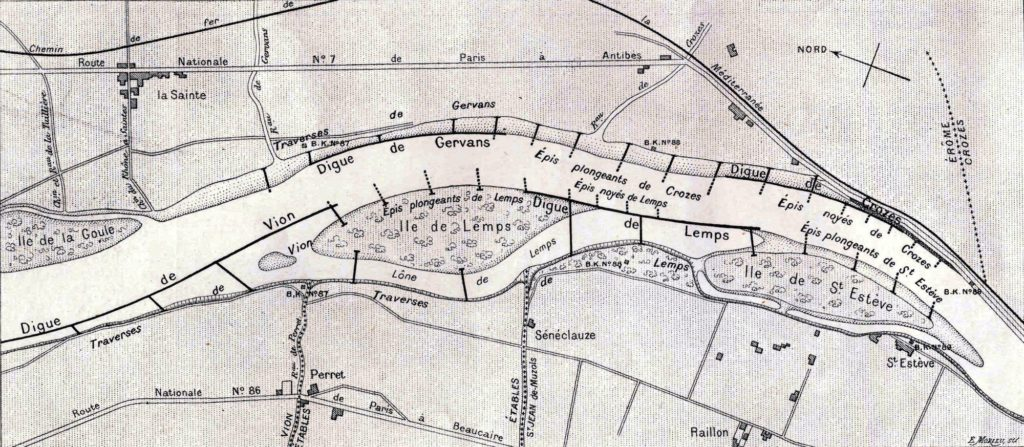
\includegraphics[width=\linewidth]{Figures/EpisGirardonGervans.jpg}
		\caption{}
		\label{subfig:Girardon}
		\end{subfigure}	
		\begin{subfigure}{0.5\linewidth}
		\centering
		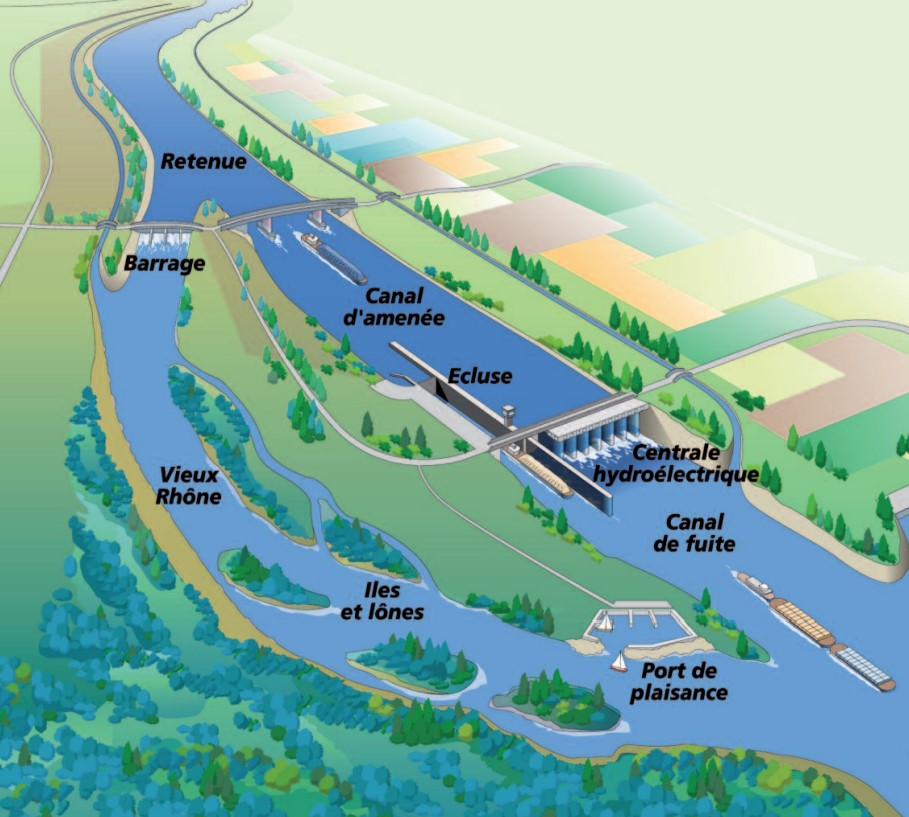
\includegraphics[width=\linewidth]{Figures/AmenTypeCNR.jpg}
		\caption{}
		\label{subfig:SchemaCNR}
		\end{subfigure}
		\caption{(a) Carte des épis et casiers Girardon installés sur le Rhône au niveau de la commune de Gervans (environ 150 km à l'amont de Beaucaire). L'objectif est de concentrer l'écoulement dans le chenal principal et de le déconnecter des chenaux secondaires ou "lônes" (source : \url{www.capsurlerhone.fr}). (b) Schéma type d'un aménagement hydroélectrique du Rhône (source : CNR).}
	\end{figure}		

	\FloatBarrier
		
	\subsubsection{Sélection d'événements de crue}
	
	\paragraph{} Pour étudier le temps de propagation des crues entre Lyon et Beaucaire, il faut tout d'abord isoler les événements qui proviennent de l'amont de Lyon. Afin de faciliter l'identification de la pointe de crue à l'aval de la zone, il est préférable qu'aucun affluent entre Lyon et la mer ne soit lui aussi en crue. Ces conditions sont réunies pour les crues océaniques décrites par \citet{parde_regime_1919} : "\textit{Les crues océaniques du Bas Rhône sont dues à un double ou même à un triple flot : celui de l'Isère, celui du Rhône supérieur, celui de la Saône. Le flot de l'Isère est ordinairement négligeable en comparaison des deux autres}". Ce type de crue est associé à des événements pluvieux qualifiés eux aussi du titre "océanique" et qui surviennent généralement durant la saison automnale ou hivernale \citep{parde_regime_1925}. Lors d'événements de crue de magnitude importante, les échanges entre les écoulements du lit mineur et ceux du lit majeur ont un impact sur la dynamique de la crue. Afin de faciliter l'analyse du déplacement de l'onde de crue, les événements non-débordants sont privilégiés. Cette analyse se limitera donc au temps de propagation des crues océaniques dont le débit à Lyon est inférieur au débit de période de retour de 20 ans, et dont l'identification à Beaucaire n'est pas biaisée par des crues des affluents intermédiaires. 
	
	\paragraph{} Les données limnimétriques disponibles à Beaucaire décrites dans les sections précédentes consistent en des enregistrements continus de la hauteur d'eau depuis 1816, au pas de temps journalier (une mesure par jour à midi) jusqu'en 1885, puis trois mesures par jour jusqu'en 1967. A partir de 1970, les mesures sont automatisées et effectuées a minima toutes les heures. Pour la partie amont de la zone d'étude, la première station à l'aval de la confluence avec la Saône a été choisie. Il s'agit de la station située à Ternay, à une quinzaine de kilomètres à l'aval de Lyon. Celle-ci était à l'origine installée à la Mulatière, quelques kilomètres à l'amont de Ternay, où des relevés journaliers (une mesure par jour à midi) existent au moins à partir de 1840. La station a par la suite été déplacée de nombreuses fois comme décrit dans le tableau \ref{tab:Hternay}. Une lacune existe autour de la seconde guerre mondiale, entre 1935 et 1949. 
	
	\begin{table}[h]
	\centering
	\caption{Bilan des relevés limnimétriques disponibles aux stations de Ternay, Givors et La Mulatière.}
	\label{tab:Hternay}
%	\resizebox{\textwidth}{!}{%
		\begin{tabular}{|l|l|l|}
			\hline
			Station      & Période   & Pas de temps \\ \hline
			La Mulatière & 1840-1890 & 1/jour       \\ \hline
			Givors       & 1890-1910 & 1/jour       \\ \hline
			Givors       & 1910-1935 & 3/jour       \\ \hline
			La Mulatière & 1949-1966 & horaire      \\ \hline
			Givors       & 1966-1980 & horaire      \\ \hline
			Ternay       & 1982-2020 & horaire      \\ \hline
		\end{tabular}
%	}
	\end{table}

	
	\paragraph{} Ainsi, la période durant laquelle des relevés sont disponibles à l'amont et à l'aval de la zone d'étude s'étend de 1840 à aujourd'hui. Durant cette période, la fréquence des mesures évolue à la fois à l'amont et à l'aval pour finalement tendre vers des relevés horaires aussi bien à Ternay qu'à Beaucaire. Il va de soi que l'identification de l'heure du passage de la pointe de crue est grandement dégradée dans le cas de mesures journalières (une seule mesure par jour à midi). Les temps de propagation calculés entre 1840 et 1910 sont de ce fait biaisés.
	
	
\FloatBarrier
	\subsubsection{Compilation du temps de propagation des crues}

	
	\paragraph{} Ce sont finalement les temps de passage de 121 crues de type océanique et non-débordantes qui sont compilés de 1840 à 2015 (Annexe \ref{sec:TabPropag}). Le temps de propagation calculé représente le délai entre l'instant du passage du pic de crue à l'amont (stations de La Mulatière, Givors ou Ternay selon la période) et son passage à l'aval (stations de Pont de Beaucaire et Beaucaire Restitution). Les événements ont été classés en 5 périodes correspondant aux différentes phases d'aménagement du lit mineur : 
	\begin{itemize}
		\item 1 - Avant les aménagements Girardon de 1840 à 1880
		\item 2 - Pendant les travaux des aménagements Girardon de 1880 à 1920
		\item 3 - Avant les dérivations CNR de 1920 à 1952
		\item 4 - Pendant les travaux des dérivations CNR de 1952 à 1980
		\item 5 - Après l'aménagement des dérivations CNR de 1980 à 2015
	\end{itemize}

	\begin{figure}[h!]
		\centering
			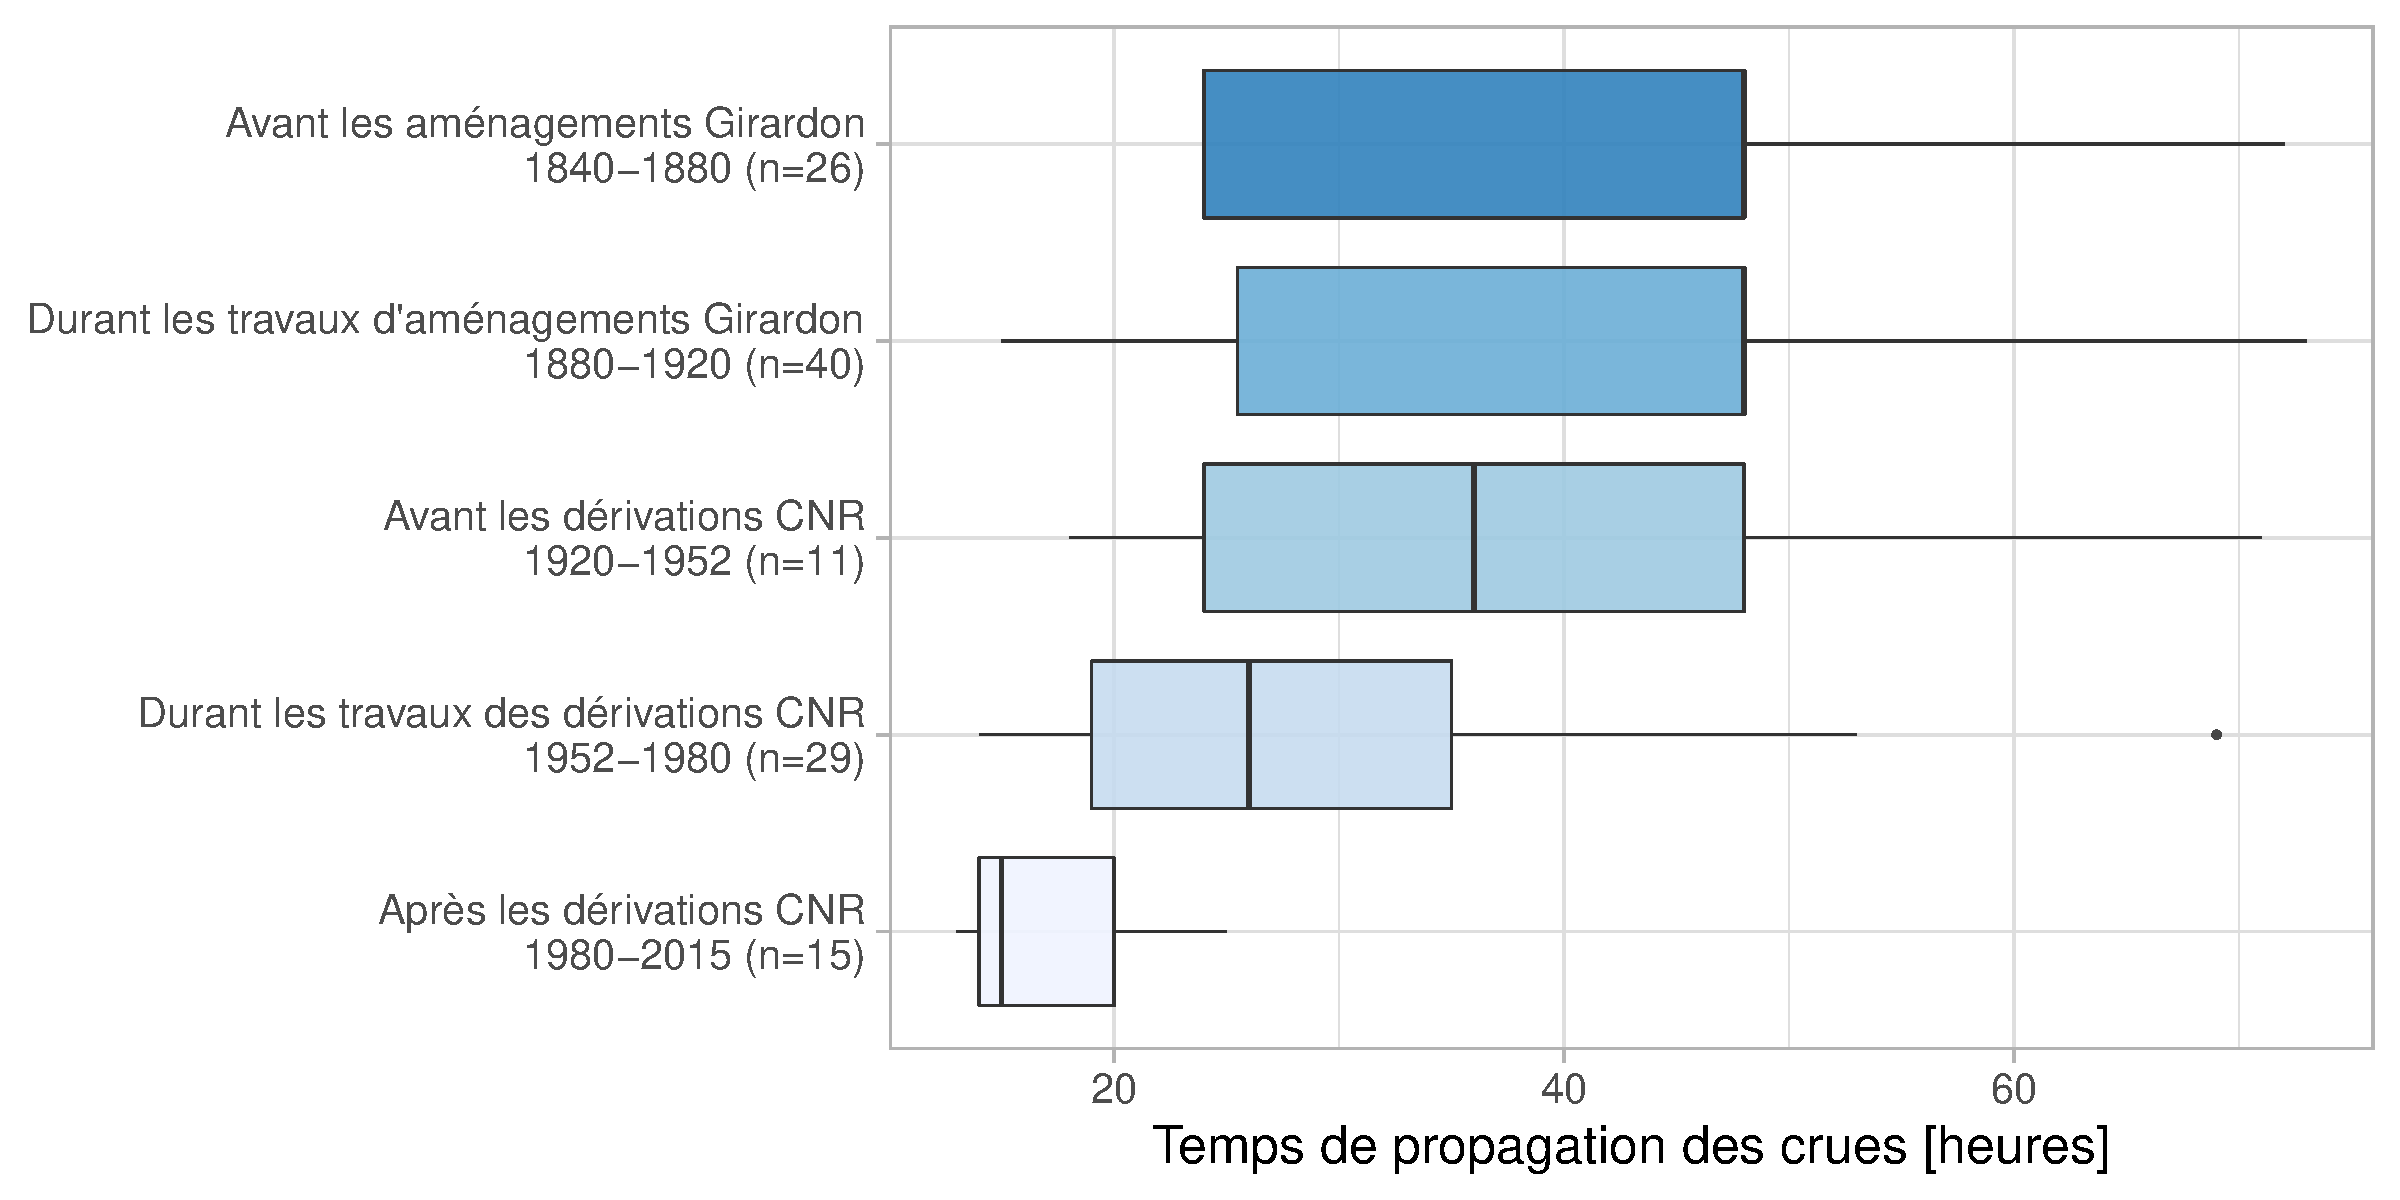
\includegraphics[width=.9\linewidth]{Figures/BoxplotTprop_Fr.pdf}
	        \caption{Boites à moustache des temps de propagation de 121 crues océaniques entre l'aval de Lyon (stations de La Mulatière, Givors et Ternay) et Beaucaire (stations de Pont de Beaucaire et Beaucaire Restitution) pour 5 périodes d'aménagement du lit mineur (1840-2015).}
			\label{fig:BoxplotPropag}
		\end{figure}	

	\paragraph{} Les résultats sont présentés dans la figure \ref{fig:BoxplotPropag}. Le temps de propagation moyen pour parcourir les 250 km qui séparent l'aval de Lyon de Beaucaire est de 35 h pour l'ensemble de la période, on constate des variations de cette durée au cours des deux siècles d'aménagement du corridor fluvial. Le temps de transfert des crues fréquentes est en constante diminution depuis le début du XIX\textsuperscript{ème} siècle. En 175 ans, il est passé de 48 h (en valeur médiane) avant la construction des casiers Girardon, à 16 h après la construction des aménagements CNR. Les ouvrages Girardon semblent avoir, dès la fin du XIX\textsuperscript{ème} siècle, amorcé la réduction de ce temps de propagation des crues. La diminution importante des temps de propagation des deux dernières périodes d'étude indique que les aménagements hydroélectriques ont eu un impact encore plus important que les premiers aménagements en lit mineur. La précision des valeurs de temps de propagation est à relativiser, principalement pour les périodes anciennes au cours desquelles les relevés limnimétriques étaient effectués une ou trois fois par jour, causant un arrondi important. Le passage à trois données par jour en 1910, puis à des données horaires à partir de 1949, permet d'améliorer la précision de l'estimation des temps de propagation. On considère cependant que la médiane de l'ensemble des événements de chaque période est un indicateur pertinent, car une sous-estimation du temps de propagation de chacun des événement est tout aussi possible qu'une sur-estimation. 
	
	\paragraph{} Afin de vérifier les calculs de temps de propagation présentés ci-dessus, un modèle hydraulique a été utilisé pour modéliser la propagation d'une crue océanique entre Lyon et Beaucaire dans les conditions actuelles. Il s'agit du modèle MAGE OSR 1D qui modélise le cours du Rhône du lac Léman à la Méditerranée. Ce modèle sera présenté plus en détails en section REF. Une crue océanique type a été modélisée en se basant sur un débit de pointe de période de retour 10 ans pour le Rhône à Lyon, et 2 ans pour la Saône et l'Isère. Le débit des autres affluents est supposé égal au module de ces derniers. Les hydrogrammes en entrée ont été constitués à partir des hydrogrammes moyens de l'étude \citet{bard_actualisation_2018} pour le Rhône à Lyon, la Saône et l'Isère. Le décalage entre les pointes de crue des trois cours d'eau est basé sur les résultats de l'étude globale du Rhône \citep{rigaudiere_etude_2000} pour les événements de crue de type océanique. Dans ce scénario, la pointe de crue de l'Isère arrive en premier, suivie 24 h plus tard par la pointe du Rhône. La pointe de crue de la Saône arrive quant à elle 5 jours après la pointe de crue du Rhône en moyenne. Suite à la modélisation de ce scénario, on obtient un temps de propagation modélisé entre Ternay et Beaucaire de 18 h, ce qui est cohérent avec les 16 h estimées par l'analyse des limnigrammes. 

	\paragraph{} Les conséquences de ces ouvrages sur la dynamique des crues peuvent être
diverses. La forme moyenne des hydrogrammes peut avoir été modifiée et le pic de crue amplifié par une propagation devenue plus rapide. De plus, la concomitance du pic de crue du Rhône avec celui de ses affluents peut avoir été modifiée. Par exemple, les pics de crue de la Saône et de l'Isère sont systématiquement en retard sur celui du Rhône dans la plupart des scénarios de crue, y compris les crues de type océanique (\cite{parde_regime_1925}; \cite{rigaudiere_etude_2000}). Si le temps de propagation des crues du Rhône est réduit, alors l'écart de temps entre le pic de crue du Rhône et celui des affluents est augmenté, entrainant un débit moins important dans la partie aval du bassin versant. Ces conséquences pourraient être étudiées plus précisément en analysant les temps de propagation au niveau de stations limnimétriques intermédiaires dans la zone étudiée.

	\paragraph{} Le Rhône n'est pas le seul fleuve qui a subi ce type de transformations. Selon \citet{mitkova_analysis_2005}, des conséquences similaires ont été observées sur les crues du Danube. Entre 1899 et 2002, le temps de propagation entre Passau et Kienstock est passé de 40 h à seulement 15 h. C'est également le cas du Pô en Italie, qui a vu le temps de propagation de ses crues réduit suite à la construction d'aménagements en lit mineur \citep{di_baldassare_analysis_2009}. Toutefois, les limites de ces études proviennent de la disponibilité et de la fiabilité des données limnimétriques historiques datant d'avant les aménagements. C'est pourquoi l'étude des temps de propagation basée sur les limnigrammes anciens est peu répandue dans la littérature, contrairement aux études basée sur la modélisation hydraulique.
	
	\paragraph{} L'impact des aménagements sur la forme et le débit de pointe des crues n'a pas été quantifié ici. Il faudra garder à l'esprit lors de l'utilisation des données pour l'analyse fréquentielle que l'homogénéité des débits maximum annuels devra être vérifiée. Si des ruptures sont détectées dans les séries de débit, elles pourront notamment être attribuées à ces modifications anthropiques de la dynamique des crues. Cependant, l'impact de la diminution des temps de propagation sur le débit de pointe des crues peut être compensé par la moins bonne concomitance avec les affluents tel que décrit précédemment.

\FloatBarrier

\section{Données historiques : la base de données HISTRHÔNE (1300-2000)}

	\subsection{Présentation de la base de données}

	\paragraph{} La base de données HISTRHÔNE (\url{histrhone.cerege.fr}) \citep{pichard_sept_2014} regroupe près de 1500 événements hydro-climatiques, depuis le XIII\textsuperscript{ème} siècle jusqu'à l'an 2000. Cet important travail d'archives qui s'est étalé sur plusieurs décennies, représente un apport majeur pour la connaissance de l'histoire hydrologique et climatique de la basse vallée du Rhône. La zone couverte par la base de données s'étale de la ville de Pont-Saint-Esprit jusqu'à la mer Méditerranée, en incluant les villes d'Avignon, Beaucaire et Arles, ainsi que l'ensemble de la Camargue (figure \ref{fig:MapHistrhone}). 
	
	\begin{figure}[h]
	\centering
		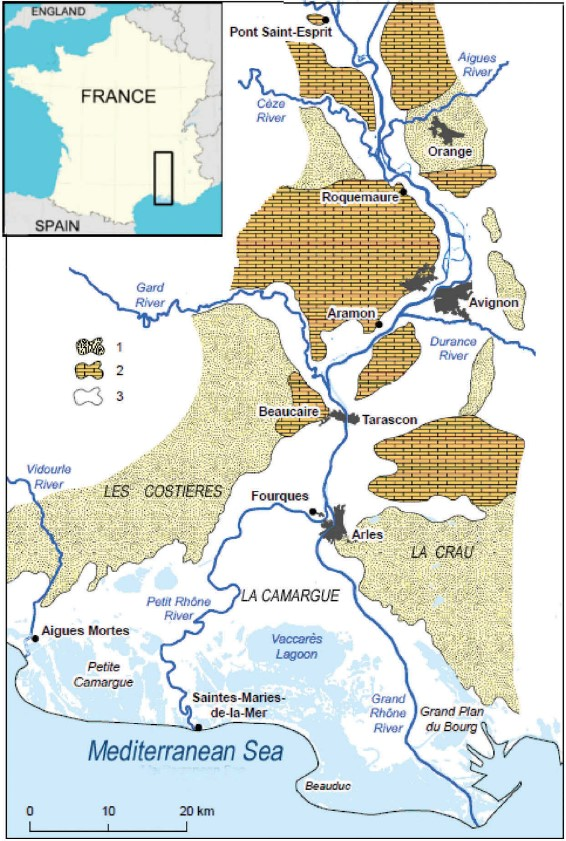
\includegraphics[width=.5\linewidth]{Figures/HistrhoneMap.jpg}
        \caption{Localisation de la zone géographique couverte par la base HISTRHÔNE \citep{pichard_sept_2014} }
		\label{fig:MapHistrhone}
	\end{figure}
	
	\paragraph{} Les éléments historiques (témoignages, cartes...) qui correspondent à un même événement hydroclimatique sont regroupés et ces événements sont classés par type dans la base de données : crue, étiage, présence de glace ou gel du Rhône, inondation pluviale, submersion marine... Au-delà de la base de données, l'ouvrage "\textit{Sept siècles d'histoire hydroclimatique du Rhône d'Orange à la mer}" \citep{pichard_sept_2014} "\textit{offre une vue synoptique, à la fois des sources, de leur critique et des perspectives ouvertes par les premiers résultats que les auteurs ont pu en tirer comme contribution à une histoire hydroclimatique}". Il faut ajouter qu'une chronologie générale des événements est disponible, ainsi qu'une étude détaillée des échelles limnimétriques du bas Rhône qui "\textit{reprend l'ensemble des problèmes de mesures de hauteurs des crues dans l'histoire et tente de résoudre ces complications pratiques de métrologie}" \citep{pichard_hauteurs_2013} .
	
	\paragraph{} Dans la base de données HISTRHÔNE, les événements de crue sont classés en 6 catégories présentées dans le tableau \ref{tab:CatCrueHistrhone}. Ces catégories correspondent à différents niveaux de gravité, allant d'un Rhône "pleins bords" jusqu'à l'inondation extraordinaire. D'après \citet{pichard_sept_2014}, ces catégories permettent le classement des crues même en l'absence d'informations sur les hauteurs ou les débits : "\textit{Un seuil de hauteur unique présente l'intérêt de la simplicité et de l'universalité. On peut ainsi choisir la limite évidente du débordement hors du lit mineur, surtout si cette limite est bien connue et sans ambiguïté, mais il faut alors renoncer à pondérer des types de crues que les sources anciennes ne permettent pas de discriminer. [...] il faut se résoudre à choisir le type de crue en fonction de critères indirects, mais tout aussi pertinents que les hauteurs et les débits. On s'appuie sur la comparaison avec la période des hauteurs mesurées en continuité, mais aussi sur les conséquences et les dommages, sur l'extension de la crue dans la plaine proximale ou distale, sur sa généralisation dans une partie ou la totalité du territoire étudié}". Si la détermination d'un seuil de hauteur ou de débit n'est pas essentielle pour l'analyse de l'historique hydroclimatique, elle l'est en revanche pour l'utilisation de ces données dans le cadre de l'analyse fréquentielle des crues.  Il faudra donc veiller à la correspondance entre ces catégories basées sur des informations très diverses.
	
\begin{table}[h]
	\centering
	\caption{Classification des événements de crues de la base HISTRHÔNE. Les estimations de débit proviennent de \citet{pichard_hydro-climatology_2017}. Les ségonnaux représentent des parcelles potentiellement exploitables comprises entre un fleuve et ses digues.}
	\label{tab:CatCrueHistrhone}
%	\resizebox{\columnwidth}{!}{
		\begin{tabular}{|m{0.8cm}|m{3.6cm}|m{7.5cm}|m{3.4cm}|}
		\hline
		Code &
		  Libellé &
		  Description &
		  Débit estimé [m\textsuperscript{3}/s] \\ \hline
		Ci &
		  Crue de gravité indéterminée &
		  Crue sans aucune précision : pas d'indice de débordement ni de gravité (incertitude totale) &
		  X \\ \hline
		Cd &
		  Crue avec indice de débordement &
		  Débordement avéré mais sans précision relative à son étendue ou sa gravité (incertitude partielle) &
		  X \\ \hline
		C1 &
		  Hautes eaux &
		  
\textbf{Rhône "pleins bords", "gros Rhône" sans débordement}. Le Rhône reste dans son lit mineur mais implique une surveillance constante aux digues &
		  X \\ \hline
		C2 &
		  Crue avec débordement sans gravité et/ou localisé &
		 
\textbf{Débordement limité}, sans gravité majeure ou bien localisée (ségonnaux, prés/chemins inondés, eaux sur les quais, dégâts mineurs sur digues) &
		 5200 \\ \hline
		C3 &
		  Crue et inondation de gravité intermédiaire &
		  
\textbf{Inondation notable} avec dégâts avérés au caractère destructeur et/ou extension de crue &
		  7200 \\ \hline
		C4 &
		  Crue et inondation extrêmes &
\textbf{Inondation extraordinaire} avec dégâts exceptionnels (pertes humaines et animales, intérieurs des villes inondés, dégradations de digues en grand nombre) et extension de crue &
		  9000 \\ \hline
		\end{tabular}
%	}
\end{table}
	
\FloatBarrier

	\subsection{Ordre de grandeur du débit de pointe des crues de la base HISTRHÔNE}
	
	\paragraph{} L'exploitation des crues historiques pour l'analyse fréquentielle nécessite d'estimer un ordre de grandeur du débit de pointe de ces événements. Plus précisément, il est possible d'exploiter statistiquement les données historiques à condition d'en déterminer un seuil de perception. Il s'agit ici de garantir que toutes les crues dont le débit fut supérieur à un seuil de perception ont laissé une trace dans les archives. Dans le cas des événements de la base HISTRHÔNE, il est possible de faire correspondre un seuil de perception à chacune des catégories. L'analyse fréquentielle des crues qui découle de ces seuils de perception sera réalisée au chapitre 4 (REF), mais il faut tout d'abord en faire une première estimation. \citet{pichard_hydro-climatology_2017} en donnent un premier ordre de grandeur (tableau \ref{tab:CatCrueHistrhone}) en calculant la moyenne du débit à Beaucaire des crues de chaque catégorie pour les événements du XX\textsuperscript{ème} siècle, en utilisant les données de la banque Hydro (\url{www.hydro.eaufrance.fr}). Néanmoins, l'utilisation d'une moyenne ne reflète pas exactement le concept de seuil de perception présenté plus tôt, mais cela permet d'en connaitre l'ordre de grandeur. Le débit de la plus petite crue de chacune des catégories serait plus adapté. 
	
	\begin{figure}[h]
	\centering
		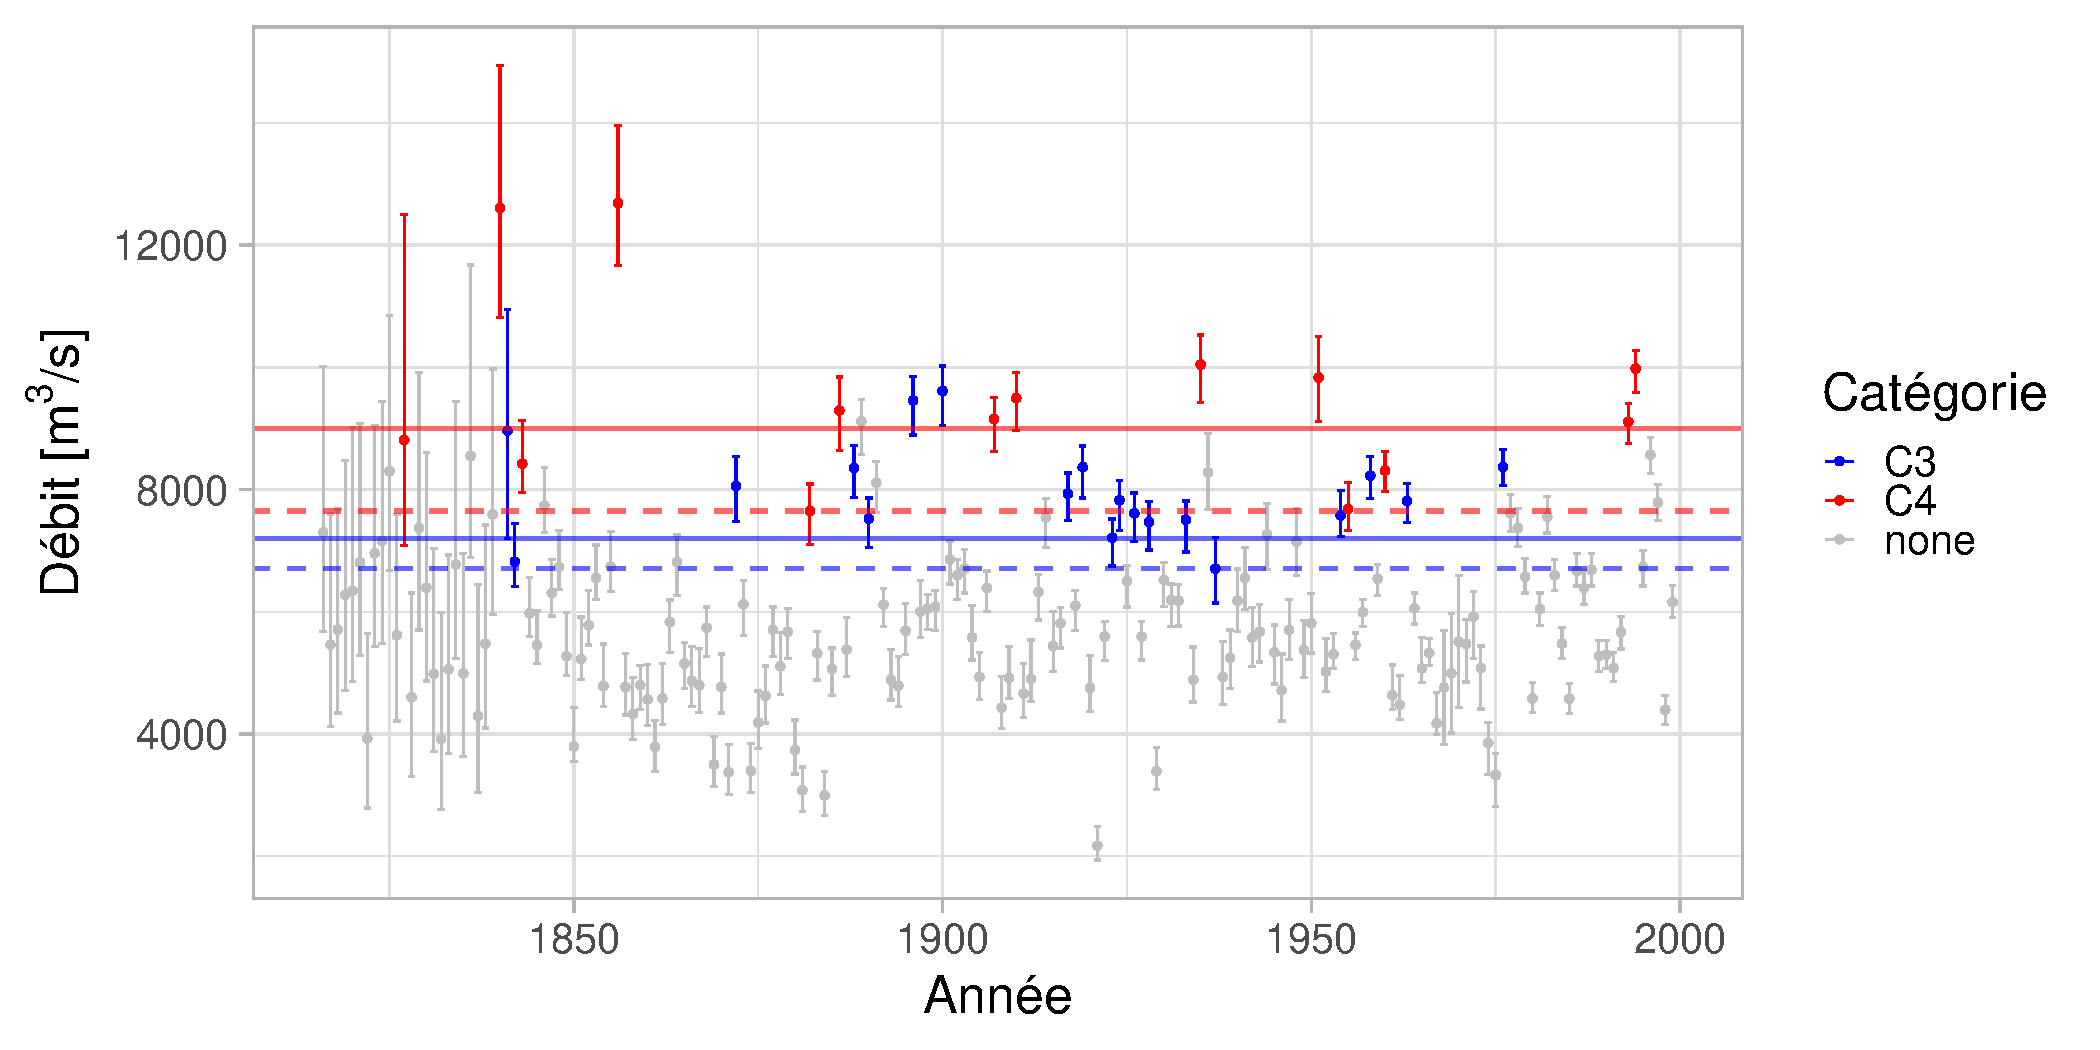
\includegraphics[width=.9\linewidth]{Figures/C3-C4_SystematicPeriod-FR.pdf}
        \caption{Débit maximum annuel à Beaucaire de 1816 à 2000 (estimations chapitre 3 REF). Les barres d'erreur représentent l'incertitude à 95\%, les droites horizontales représentent l'estimation de \citet{pichard_hydro-climatology_2017} (trait plein) et le débit maxpost de la plus petite crue de chacune des catégories (trait pointillé).}
		\label{fig:C3-C4_Syst}
	\end{figure}
		
	
	\paragraph{} Les débits maximum annuels avec incertitude de 1816 à 2020 (dont le calcul sera détaillé au chapitre 3 (REF)) sont croisés avec les catégories C3 et C4 de la base HISTRHÔNE. La période commune de ces deux jeux de données s'étend de 1816 à 2000. Seules ces deux catégories sont retenues car elles contiennent des crues responsables de dégâts notables et sont susceptibles d'être informatives pour l'analyse fréquentielle menée au chapitre 4 (REF). On remarque sur la figure \ref{fig:C3-C4_Syst} que les limites entre catégories sont "perméables", du moins pour cette période "témoin" de 1816 à 2000 : des crues appartenant à la catégorie C3 sont plus fortes que certaines crues de la catégorie C4. Par exemple, le débit maximum de l'année 1900, classée C3, atteint 9614 m\textsuperscript{3}/s, alors que les 8310 m\textsuperscript{3}/s de l'année 1960 sont classés en catégorie C4. A ce propos, \citet{pichard_sept_2014} expliquent que : "\textit{Ce sont les catégories C3 et C4 qui offrent les plus grandes difficultés de discrimination. Pour la catégorie C3, la distinction avec les crues localisées est parfois délicate [...] Il y a une gradation certaine au sein de cette catégorie [...] Ce sont ainsi les crues dites extrêmes qui permettent de délimiter les passages dans la catégorie supérieure, beaucoup plus nette. Les crues extrêmes (C4) entrainent des destructions importantes, s'introduissent au cœur des villes et dans les maisons, couvrent des territoires les plus étendus et transforment la Camargue et le Plan du Bourg d'Arles en mers à perte de vue.}" De plus, certaines crues ne sont pas classées bien que supérieures à certaines crues C4. Par exemple, le débit maximum annuel de l'année 1889 atteint 9115 m\textsuperscript{3}/s mais n'est classé dans aucune des deux catégories, alors que la plus petite des crues de la catégorie C4 n'atteint que 7649 m\textsuperscript{3}/s (1882). 
	
	\paragraph{} La moyenne des crues de chaque catégorie sur la période 1816-2000 est plus forte que celle présentée par \citet{pichard_hydro-climatology_2017} car cette dernière est calculée uniquement sur les données XX\textsuperscript{ème} siècle (tableau \ref{tab:Qcateg}). Ces valeurs moyennes permettent d'avoir un ordre de grandeur du débit de ces catégories mais ne répondent pas à la définition du seuil de perception. Le débit de la plus petite crue de chaque catégorie représente une estimation plus adéquate, même si les limites entre catégories ne semblent pas univoques en terme de débit. Ces constatations encouragent la considération d'une incertitude autour du seuil de perception. De plus, le fait que certains débits maximum annuels supérieurs à la plus petite des crues C4 (1816-2000) ne correspondent à aucune des deux catégories encourage à la méfiance quand à l'exhaustivité des données sur l'ensemble de la période. Ces questions d'incertitudes autour du seuil de perception et de l'exhaustivité des données historiques seront abordées plus en détails dans le chapitre 4 (REF).

	\begin{table}[h]
	\centering
	\caption{Débits caractéristiques des catégories de la base HISTRHÔNE. Les estimations de \citet{pichard_hydro-climatology_2017} représentent la moyenne des débits maximum annuels du XX\textsuperscript{ème} siècle. Les autres colonnes correspondent à la moyenne des débits maximum annuels de chaque catégorie et le débit de la crue la plus petite de chacune des catégories basés sur la chronique continue estimée de 1816 à 2000 au chapitre 3 (REF).} 
	\label{tab:Qcateg}
		\begin{tabular}{|c|c|c|c|}
		\hline
		Catégorie HISTRHÔNE & \citet{pichard_hydro-climatology_2017} & Moyenne 1816-2000 & Minimum 1816-2000\\ \hline
		C3  & 7200 m\textsuperscript{3}/s  & 7970 m\textsuperscript{3}/s    & 6706 m\textsuperscript{3}/s   \\ \hline
		C4  & 9000 m\textsuperscript{3}/s  & 9506 m\textsuperscript{3}/s    & 7649 m\textsuperscript{3}/s   \\ \hline
		\end{tabular}
	\end{table}
	
	\subsection{Évolution temporelle de la vulnérabilité aux inondations}
	\label{subsec:EvolVuln}
	
	\paragraph{} Le classement des crues dans la base HISTRHÔNE est basé sur des critères indirects, différents du débit et de la hauteur d'eau, tels que : "\textit{les conséquences et les dommages, [...] l'extension de la crue dans la plaine proximale ou distale, [...] sa généralisation dans une partie ou la totalité du territoire étudié}" \citep{pichard_sept_2014}. Les mêmes critères sont utilisés pour catégoriser les crues du XIV\textsuperscript{ème} siècle et celles du XX\textsuperscript{ème} siècle. Pourtant, la vulnérabilité des populations ripariennes évolue au cours du temps, et ce partout dans le monde \citep{kron_flood_2002}. De nombreux exemples de cette évolution existent, y compris en France, comme démontré par \citet{boudou_assessing_2016} pour les bassins versants du Doubs et du Tarn. La basse vallée du Rhône ne fait pas exception à la règle \citep{piegay_observatoire_2022}. De plus, la perception des dommages par les populations est elle aussi variable et est la conséquence de nombreux facteurs, pouvant être d'origine physique (niveau de protection aux inondations, rupture de digues, densité de population...), médiatiques (contexte sociétal, politique, religieux...). Ainsi, on observe au sein des données de crue de la base HISTRHÔNE des fluctuations dont l'origine n'est probablement pas seulement hydroclimatique. 
	
	\begin{figure}[h]
	\centering
		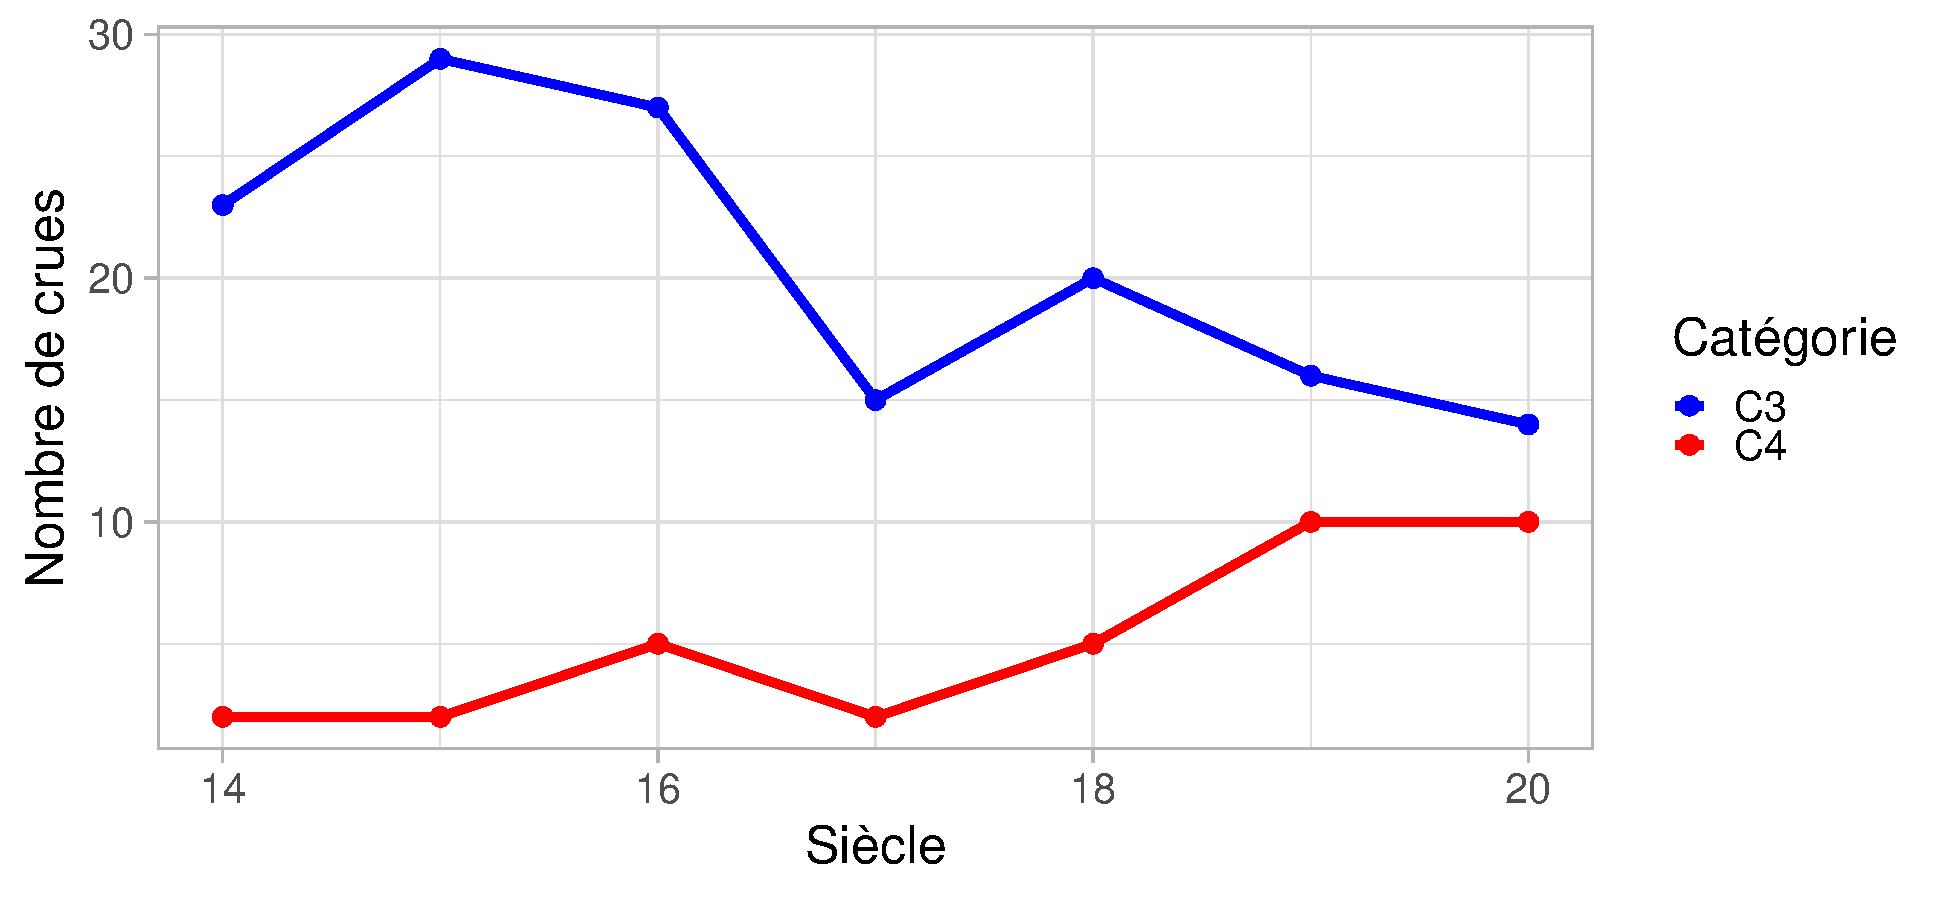
\includegraphics[width=.8\linewidth]{Figures/Nb_C3-C4.pdf}
        \caption{Nombre de crues par siècle dans les catégories C3 et C4 de la base HISTRHÔNE, du XIV\textsuperscript{ème} au XX\textsuperscript{ème} siècle.}
		\label{fig:Nb_C3C4}
	\end{figure}	
	
	\paragraph{} La figure \ref{fig:Nb_C3C4} témoigne de l'évolution de la perception des crues des catégories C3 et C4. On constate une diminution du nombre de crues C3 à partir du XVII\textsuperscript{ème} siècle, au profit des crues de la catégorie C4. Plusieurs facteurs peuvent expliquer cette évolution. \citet{pichard_sept_2014} l'attribuent notamment aux actions anthropiques : "\textit{La reconstruction et l'extension des digues, le défrichement des rives, l'essor urbain, tout concourt à concentrer les écoulements lors des plus grands épisodes tout en atténuant ou même en faisant disparaître les débordements ordinaires ou moyens (C2 et C3)}".
	
\FloatBarrier

\section{Estimation du débit des événements historiques}

	\paragraph{} Dans l'optique de l'utilisation des données de crues historiques de la base HISTRHÔNE pour l'analyse fréquentielle, la connaissance du débit de chacun des événements peut s'avérer utile. Cependant, l'estimation de ces débits dans un contexte historique est bien plus complexe que dans le cas de stations hydrométriques et peut être impacté par de fortes incertitudes. Tout d'abord, la mesure limnimétrique n'est pas continue et repose sur des témoignages sporadiques, donnant des informations très dispersées spatialement. Il peut également être complexe de reconstituer la hauteur d'eau correspondant à la pointe de la crue et il est encore plus complexe de reconstituer la dynamique temporelle de la crue. Ensuite, l'estimation d'un débit basée sur la hauteur observée n'est pas évidente en l'absence de jaugeages. Le schéma hydrométrique classique ne peut donc être suivi. Une des solutions est l'utilisation d'un modèle hydraulique. Cependant, l'élaboration d'un tel modèle est notamment conditionnée à l'existence ou à la reconstitution de données topographiques et bathymétriques contemporaines à la crue étudiée. La modélisation hydraulique unidimensionnelle (1D) est très simplifiée car elle fait l'hypothèse que les quantités (hauteur d'eau, vitesses et direction de l'écoulement) sont uniformes au sein d'une section en travers. Ce type de modèle n'est pas aussi précis qu'un modèle 2D, mais il demande en revanche une description bien moins fine de la géométrie de la rivière, ce qui est avantageux dans le cas de reconstitutions historiques pour lesquelles ces données sont rares. Le but de l'utilisation de la modélisation hydraulique dans ce chapitre est l'inverse du but habituel. En effet, on cherche ici à identifier le débit ayant engendré les niveaux d'eau relevés lors des crues, et non à estimer les niveaux atteints pour un débit donné. Pour cela, il est possible pour un événement donné d'encadrer le débit de la crue dans un intervalle, en approchant la hauteur d'eau atteinte en un point donné qui est extraite de la base HISTRHÔNE avec la hauteur modélisée en ce même point. Dans la section qui suit, la piste de l'estimation du débit des crues historiques par la modélisation hydraulique 1D est explorée afin d'évaluer si les limites de cet exercice sont surmontables pour des événements antérieurs à l'installation de l'échelle limnimétrique de Beaucaire. Ces estimations de débit pourraient ensuite être utilisées dans le cadre l'analyse fréquentielle des crues. Des hypothèses simplificatrices du modèle hydraulique seront notamment explorées afin de limiter la quantité d'informations nécessaires.

	\FloatBarrier
	 \subsection{Adaptation du modèle MAGE OSR 1D à l'étude des crues historiques à Beaucaire}
	 
	 \paragraph{} L'Observatoire des Sédiments du Rhône (OSR) (\url{www.graie.org/osr}) étudie les flux sédimentaires ainsi que les pollutions associées à ces sédiments sur les 545 km du cours du Rhône du lac Léman à la Méditerranée. A ce titre, un modèle hydraulique a été développé sur l'ensemble du linéaire (\cite{dugue_accounting_2015}; \cite{launay_numerical_2019}). Ce modèle se base sur le code de calcul MAGE \citep{souhar_approach_2009} qui résout les équations de Barré-de-Saint-Venant 1D ainsi que la formule de perte de charge de Manning-Strickler. Le modèle inclut également les tronçons les plus à l'aval des principaux affluents, ainsi qu'une représentation du fonctionnement des aménagements hydroélectriques. Il a été calé et validé jusqu'au débit des crues non-débordantes (soit un débit de période de retour d'environ 10 ans pour la partie à l'aval de Lyon). La géométrie du lit est définie par des profils en travers réalisés environ tous les 500 m. Le modèle n'étant pas prévu pour représenter les crues débordantes, les profils en travers s'étendent jusqu'aux limites du lit moyen, aussi appelé lit majeur actif (c'est-à-dire la partie mouillée par les crues fréquentes). Les débordements, ruptures de digues et surverses ne sont donc pas pris en compte (sauf quelques exceptions locales) et la géométrie au-delà des digues est représentée par des murs verticaux artificiels dont les frottements sont négligés. 
	 
	 \paragraph{} Le modèle MAGE OSR 1D est adapté à l'étude de la dynamique hydro-sédimentaire à long terme, mais ne peut en l'état être utilisé pour la modélisation des crues à Beaucaire : plusieurs adaptations et hypothèses simplificatrices sont nécessaires. Tout d'abord, il est inutile de conserver la totalité des biefs, le modèle s'étendant du lac Léman à la Méditerranée. Afin de limiter la quantité de données anciennes nécessaire, ainsi que le temps de calcul, la limite amont du modèle est définie à l'aval immédiat de la confluence avec la Durance, environ 15 km à l'amont de Beaucaire. La limite amont aurait pu être fixée à la confluence avec le Gardon (dernier affluent du Rhône, 5 km à l'amont de Beaucaire). Cependant, il est complexe de reconstituer la bathymétrie historique de cette confluence notamment à cause des importants changements morphologiques suite à l'installation des aménagements CNR (figure \ref{fig:LimAmont}). Dans un but de simplification, le Gardon sera représentée par un apport latéral direct dans le modèle, ce qui ne nécessite pas la reconstitution de sa bathymétrie. 
	 
	 \begin{figure}[h]
		\centering
	    \includegraphics[width=.9\linewidth]{Figures/LimAmont.pdf}
        \caption{Confluence du Gardon et du Rhône environ 5 km à l'amont de Beaucaire pour la période pré-aménagements CNR à gauche (carte IGN 1950) et la période actuelle à droite (carte IGN actuelle). Source : \url{www.geoportail.gouv.fr}.}
		\label{fig:LimAmont}
	\end{figure}
	 
	\paragraph{} La limite aval originelle du modèle est représentée par la mer Méditerranée pour les deux biefs du delta, le Petit et le Grand-Rhône. Étant donné les fortes évolutions bathymétriques de l'embouchure du Grand-Rhône représentées sur la figure \ref{fig:Embouch} \citep{pichard_les_2014}, il serait utile de pouvoir fixer la limite aval plus à l'amont. Il existe un nombre important de hauteurs d'eau pour les crues historiques à l'échelle reconstituée des marches du port d'Arles \citep{pichard_les_1995}, la limite aval pourrait donc fixée au niveau de cette échelle, au PK 282.2, à condition que l'impact sur les hauteurs modélisées à Beaucaire soit négligeable.
	
	\begin{figure}[h]
		\centering
	    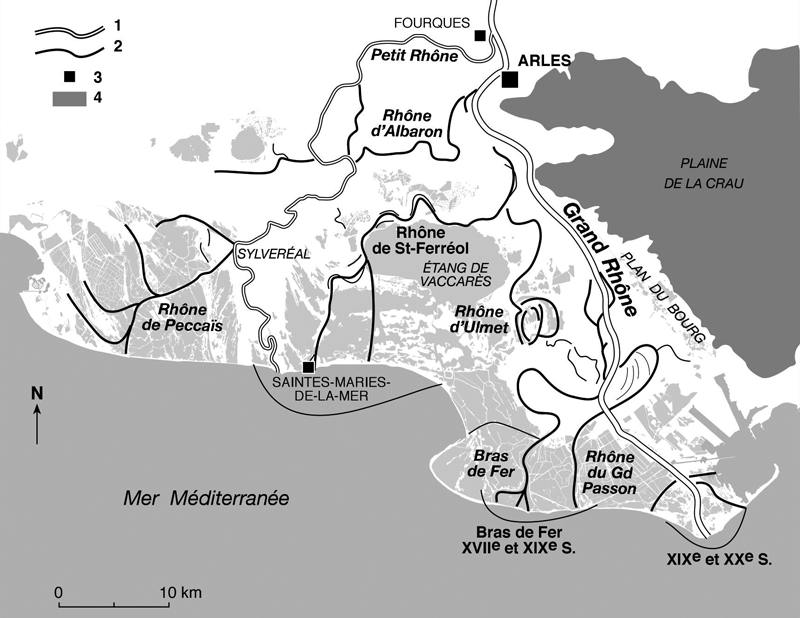
\includegraphics[width=.7\linewidth]{Figures/EvolEmbouch.jpg}
        \caption{Évolutions morphologiques du delta du Rhône du XIV\textsuperscript{ème} à aujourd'hui \citep{pichard_les_2014}). Beaucaire se situe environ 15 km à l'amont de Fourques. 1 : bras actifs de nos jours, 2 : tracés des bras hérités, 3 : Principales localités, 4 : plaine de la Crau.}
		\label{fig:Embouch}
	\end{figure}

	\paragraph{} L'influence du déplacement de la limite aval du modèle peut être étudiée. Une simulation est réalisée pour un débit constant (et non-débordant) de 4000 m\textsuperscript{3}/s en limite amont pour les deux scénarios. La figure \ref{fig:DifMerArles} présente la différence de cote (hauteur d'eau) entre les scénarios "limite aval au niveau de la mer" et "limite aval au niveau d'Arles", pour le bief reliant Beaucaire à la diffluence du Petit Rhône. On remarque que la différence est maximale au niveau de la diffluence (7 cm). A Beaucaire, la différence de hauteur est inférieure à 3 cm. On supposera donc que le choix de la limite aval au niveau du Grand-Rhône n'a que peu d'impact sur la cote à Beaucaire et que l'on pourra se passer de reconstituer les formes anciennes de la partie aval de ce bief. 
	 
	\begin{figure}[h]
	\centering
		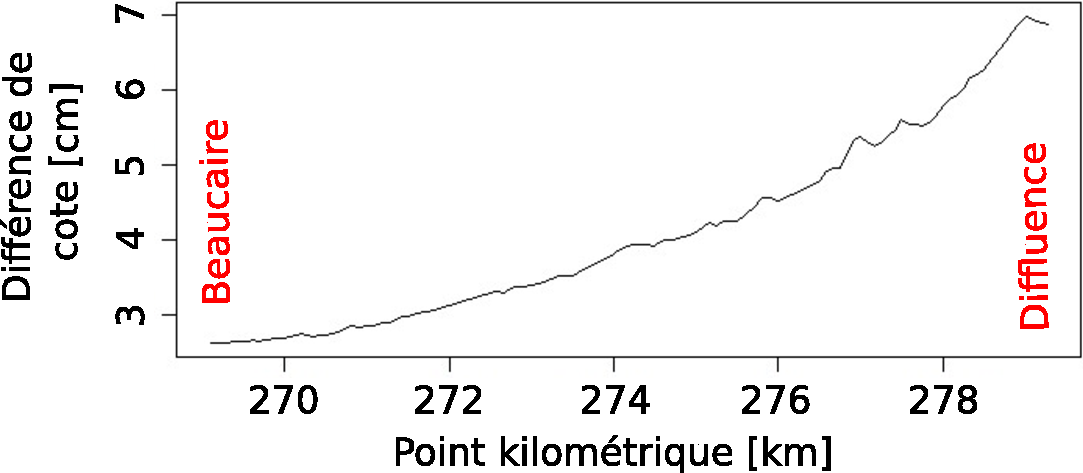
\includegraphics[width=.9\linewidth]{Figures/DiffMerArles.pdf}
        \caption{Différence de hauteur d'eau sur le bief Beaucaire-Diffluence pour une limite aval au niveau de la mer ou au niveau de la ville d'Arles. La ville d'Arles se situe environ 2 km à l'aval de la diffluence (à droite).}
		\label{fig:DifMerArles}
	\end{figure}			 
	 	
\FloatBarrier

	\paragraph{} Afin d'adapter la géométrie des sections à des débits importants, des points supplémentaires ont été ajoutés au modèle pour représenter le lit majeur. L'altitude de ces points est basée sur les données MNT de la base de données topographique (BDT) du Rhône dont les mesures ont été réalisées en 2010 dans le cadre du Plan Rhône. Les sections en travers sont prolongées jusqu'aux digues de protection actuelles (figure \ref{fig:Elarg}) qui protègent des débordements au moins jusqu'au niveau de la crue de 2003, soit une crue environ centennale. 
	
	\begin{figure}[h]
	\centering
		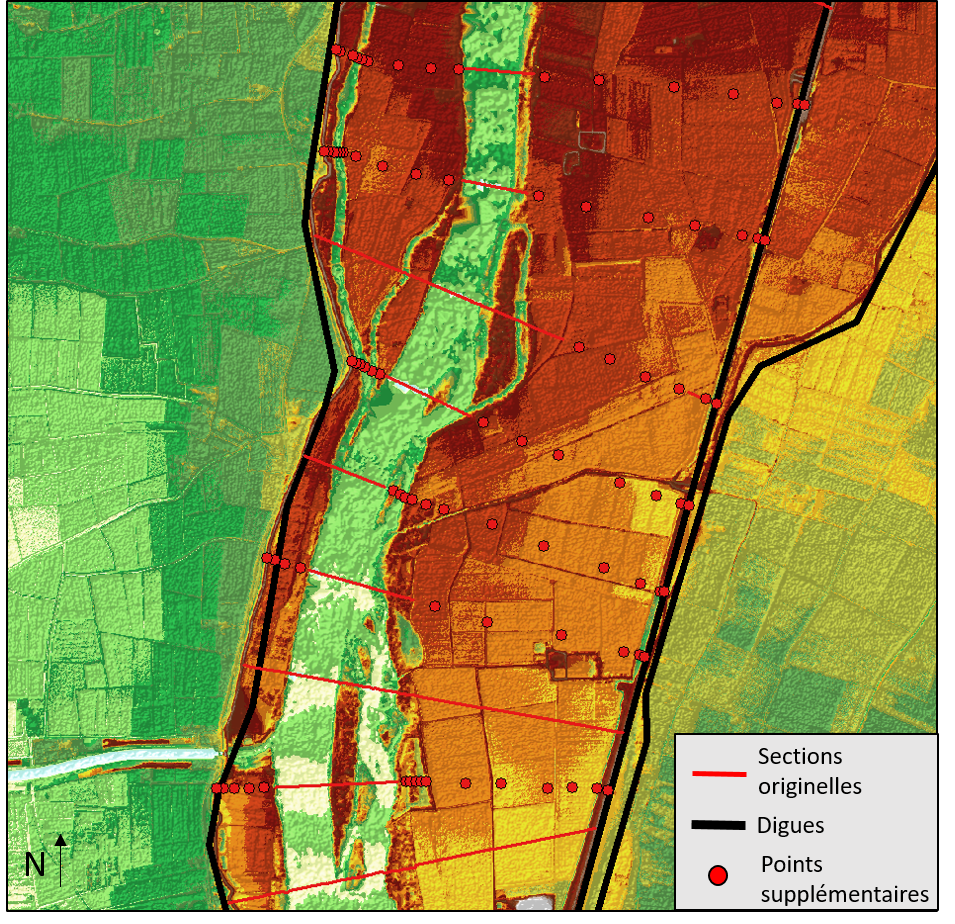
\includegraphics[width=.5\linewidth]{Figures/Elarg.png}
        \caption{Élargissement des sections en travers du modèle jusqu'aux limites du lit majeur (digues). On se trouve ici entre Beaucaire et Arles, 4 km à l'amont de la diffluence. L'altitude des points est basée sur le MNT de la BDT Rhône de 2010 qui est affiché en arrière plan. Les couleurs vertes correspondent à de faibles altitudes, les couleurs sombres à des altitudes plus importantes.}
		\label{fig:Elarg}
	\end{figure}		
	
	\paragraph{} Afin de se placer dans le contexte historique pré-aménagements CNR, les aménagements présents dans le modèle sont supprimés. Il s'agit de l'usine de Beaucaire, du barrage de Vallabrègues, ainsi que du seuil de Beaucaire. La topologie du modèle suite aux simplifications présentées dans cette section est représentée dans la figure \ref{fig:Mageavap} (droite).
	
	\begin{figure}[h]
	\centering
		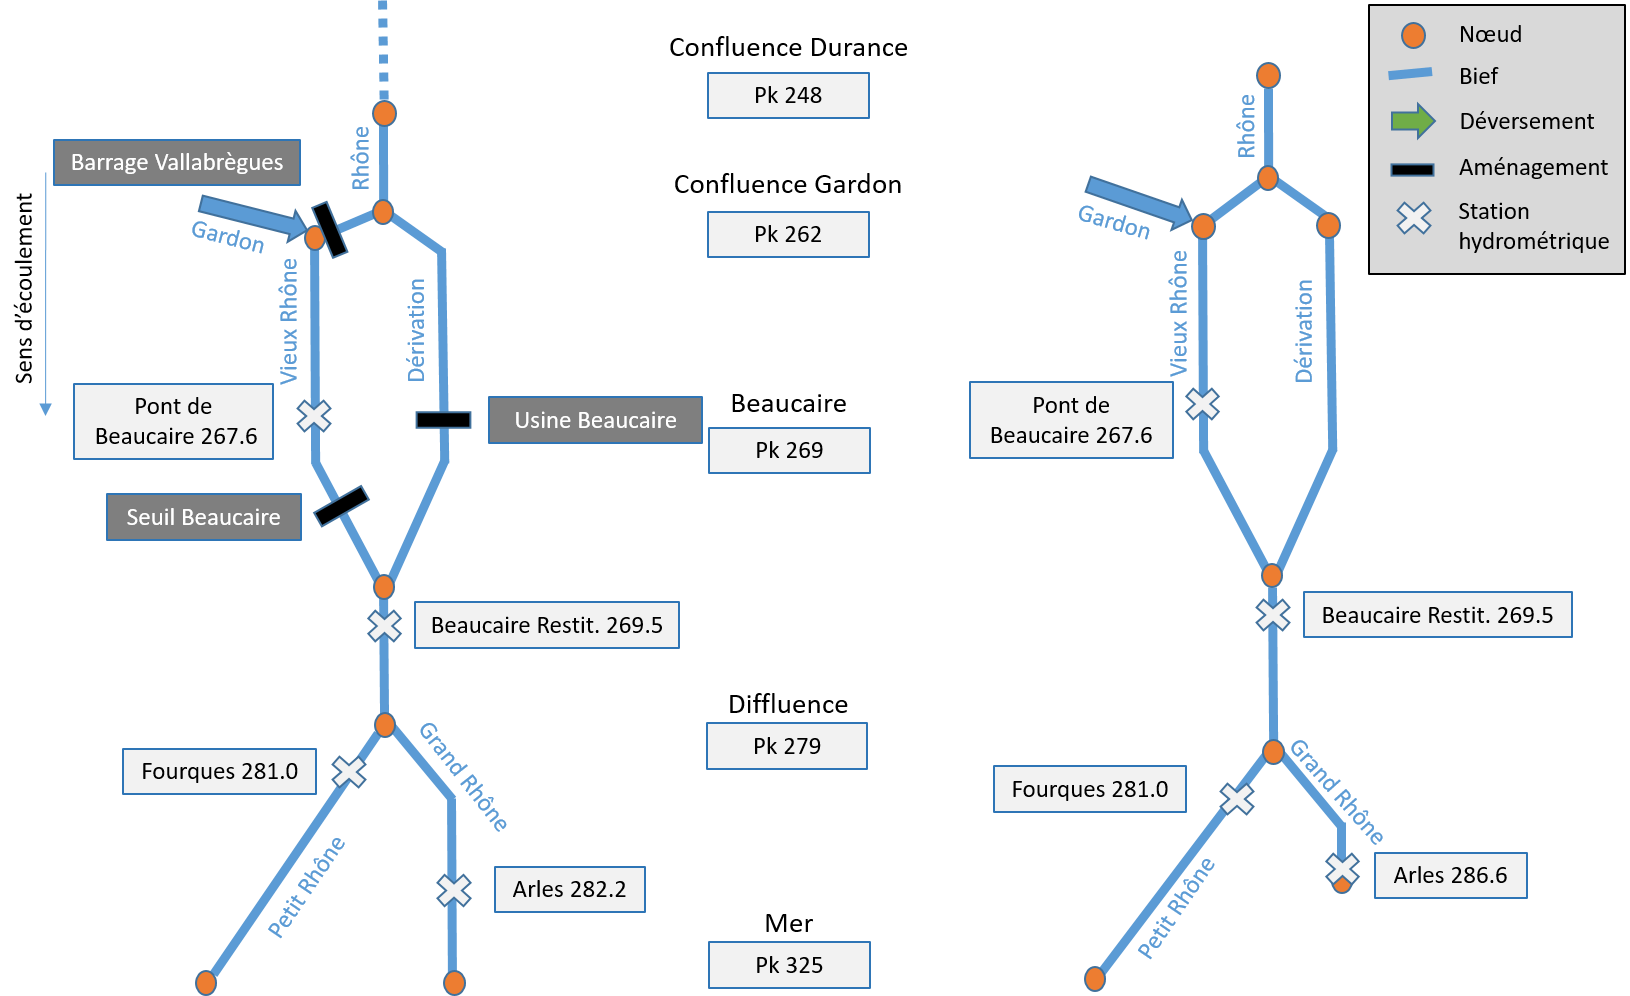
\includegraphics[width=.9\linewidth]{Figures/MAGERh_AvAp.png}
        \caption{Topologie du modèle avant (gauche) et après simplifications (droite) : suppression des aménagements récents et limite aval du bief du Grand-Rhône ramenée à Arles.}
		\label{fig:Mageavap}
	\end{figure}		
	
\FloatBarrier	
	\subsection{Simplification du modèle Rhône OSR 1D}
		
	\paragraph{} La sensibilité du modèle hydraulique à plusieurs scénarios a été testée afin de connaitre l'impact de la prise en compte (ou de la non-prise en compte) précise de ces scénarios dans le cadre de reconstitutions historiques. La référence de ces tests est le modèle présenté à la section précédente, pour lequel les aménagements hydroélectriques ont été supprimés, les sections en travers ont été élargies jusqu'aux limites du lit majeur, et la limite aval du Grand Rhône a été fixée à Arles. Les simulations suivantes représentant diverses hypothèses seront donc comparées à cette simulation de référence. La différence de hauteur au niveau de la station de Pont de Beaucaire sera notamment étudiée.
	
	\paragraph{} On cherche à reproduire ici une crue centennale similaire à la crue de décembre 2003 au cours de laquelle le débit à Beaucaire était d'environ 11 500 m\textsuperscript{3}/s \citep{medd_debit_2005}. La condition limite amont (nœud à l'aval de la confluence avec la Durance) est représentée par un hydrogramme permanent de 10 000 m\textsuperscript{3}/s. La confluence du Gardon est représentée par un apport latéral constant de 1500 m\textsuperscript{3}/s, ce qui correspond environ à une crue décennale à la station du Rémoulins, la station située la plus à l'aval sur le Gardon (\url{hydro.eaufrance.fr}). Le débit du Gardon pendant la crue de décembre 2003 a atteint environ 1250 m\textsuperscript{3}/s à Rémoulins, mais cette valeur est fortement incertaine. La limite aval pour le bief du Petit Rhône est représentée par un niveau de la mer Méditerranée de 0.136 m NGF IGN69. La limite aval du Grand Rhône est représentée par un limnigramme constant à 7.03 m NGF IGN69, soit la hauteur maximale enregistrée lors de la crue de 2003. Le calage des coefficients de frottement (Strickler) du modèle OSR \citep{launay_zabr-osr_2017} est conservé, bien que ces derniers ne soient validés que jusqu'à la crue décennale. Le pas de temps de simulation est de 60 secondes, et l'événement est simulé pendant une durée de 10 heures afin d'aboutir à une convergence satisfaisante.
	
	\begin{figure}[h]
		\centering
		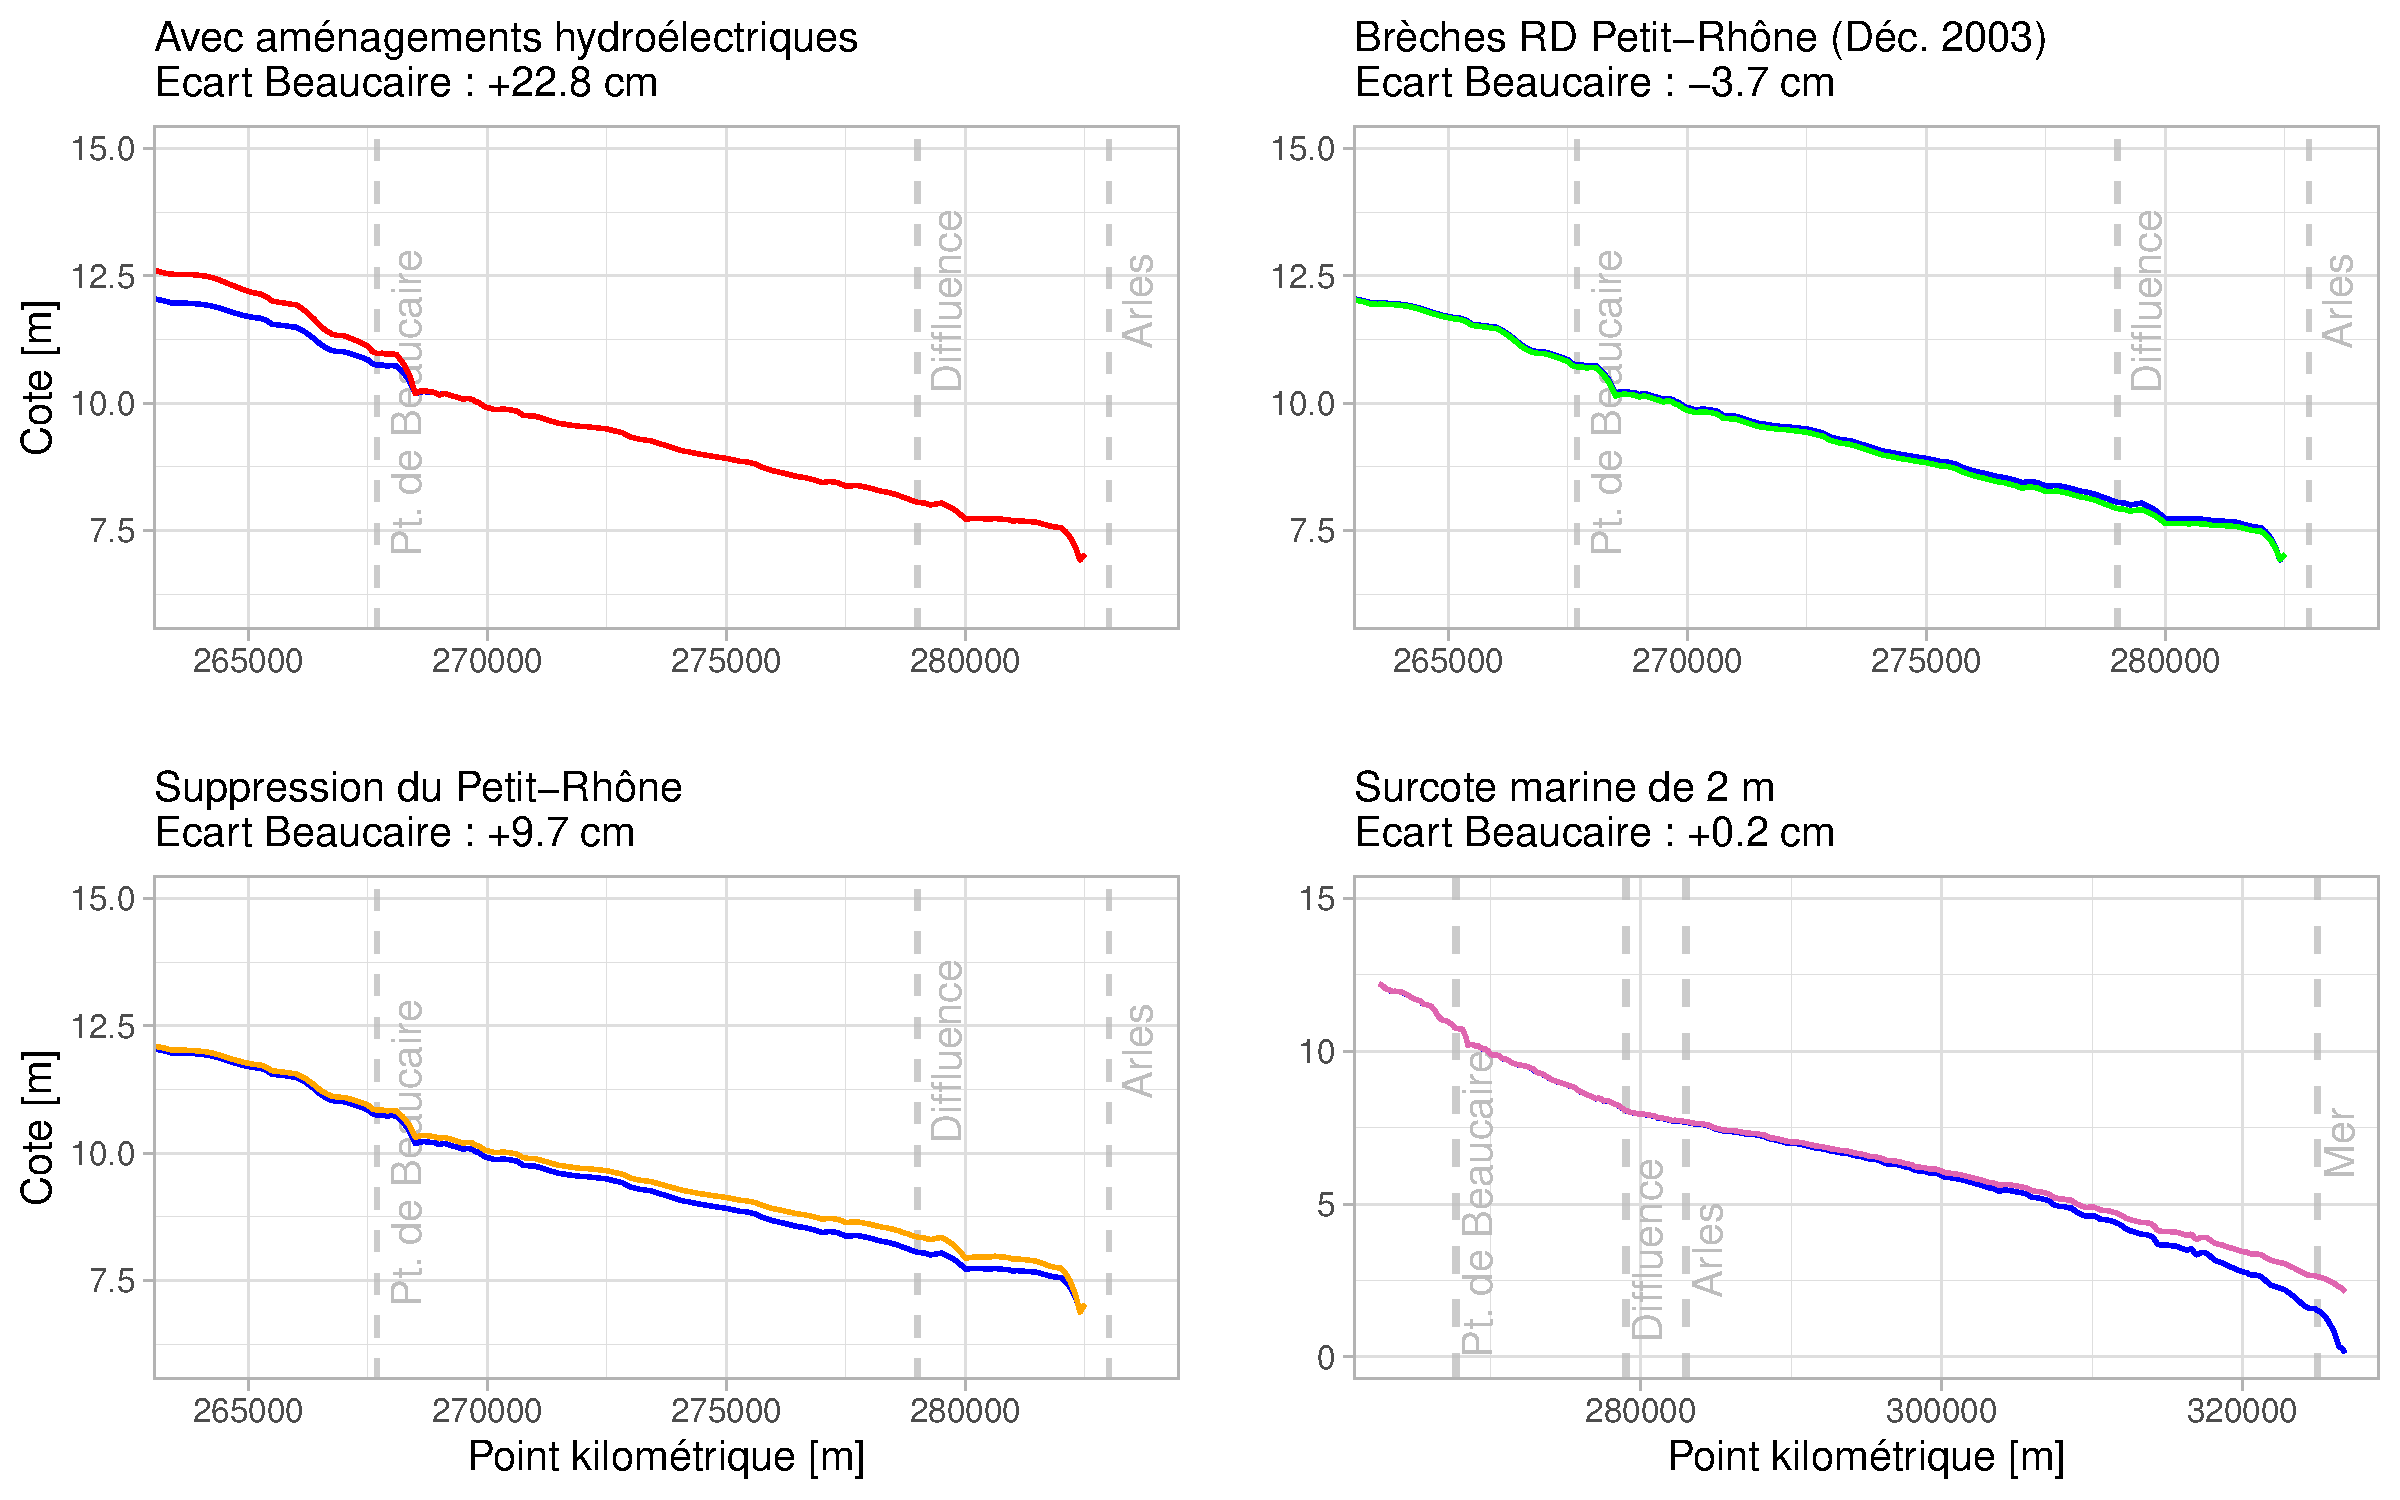
\includegraphics[width=\linewidth]{Figures/4cases.pdf}
        \caption{Lignes d'eau modélisées pour 4 scénarios, comparées à la référence (bleu), pour une crue centennale en régime stationnaire. Il s'agit des lignes d'eau des biefs Vieux Rhône-Beaucaire, Beaucaire-Diffluence, Diffluence-Arles (Grand-Rhône), excepté pour le graphique du coin inférieur droit dont le dernier bief représente le Petit-Rhône (Diffluence-Mer).}
		\label{fig:Sensib4}
	\end{figure}		
				
\FloatBarrier	

	\subsubsection{Sensibilité à la présence d'aménagements hydroélectriques}
	
		\paragraph{} Les aménagements hydroélectriques CNR ont été construits entre 1967 et 1970 et ont une influence sur la ligne d'eau à Beaucaire. Ces aménagements sont représentés dans le modèle OSR originel \citep{launay_zabr-osr_2017} sous forme de lois d'ouvrage qui seront reprises ici. Par exemple, le barrage de Vallabrègues est représenté par une loi de type seuil/déversoir avec une cote de déversement de 16.63 m, une largeur déversante de 176 m, et un coefficient de débit de 0.4. La vanne de fond est représentée par un orifice rectangulaire dont la cote de déversement correspond à un niveau de 2.03 m, la cote de mise en charge à un niveau de 6.1 m, et la cote de mise en charge maximale à un niveau de 16.6~m. L'usine hydroélectrique et le seuil de Beaucaire sont également représentés dans le modèle (figure \ref{fig:Mageavap}). La suppression des aménagements hydroélectriques dans le modèle semble avoir un impact important sur la ligne d'eau à l'amont du bief Beaucaire-Diffluence, avec une réduction de 22.8 cm de la hauteur d'eau à Pont de Beaucaire (figure \ref{fig:Sensib4}). Cela représente une différence en débit de 548 m\textsuperscript{3}/s, soit une erreur d'environ 3.5\% d'après la courbe de tarage la plus récente élaborée au chapitre 3 REF. En résumé, l'effacement des aménagements semble utile afin de ne pas sur-estimer la cote atteinte à Beaucaire pour un débit donné, même si cette sur-estimation est relativement faible. Cet effacement ne représentant pas un travail important, il est intéressant de l'effectuer. On peut cependant noter que le modèle de "référence" n'est absolument pas représentatif des conditions d'écoulement pré-aménagements CNR (avant 1967) étant donné que la géométrie des sections provient de mesures réalisées en 2010. Bien que le Rhône au droit de Beaucaire soit historiquement séparé en deux chenaux par des digues, même avant la construction des aménagements CNR (\ref{fig:CartoRes}), il faut noter que ces deux chenaux communiquaient à haut débit, ce qui n'est pas le cas ici. 
		
	\subsubsection{Sensibilité à la suppression du Petit-Rhône} 
	
	\paragraph{} La morphologie du Petit-Rhône a profondément évolué au cours des derniers siècles (figure \ref{fig:Embouch}), comme souligné par \citet{pichard_les_2014} et \citet{raccasi_mutations_2008}. De plus, la part de débit correspondant au Petit-Rhône part rapport à celle du Rhône total a probablement changé au gré de ses évolutions morphologiques. Ces changements rendent complexe la reconstitution de la morphologie historique du Petit-Rhône. Afin de s'affranchir de ces reconstitutions, la solution la plus simple et la plus radicale est la suppression du Petit-Rhône du modèle hydraulique, la totalité des débits transitant alors par le bief du Grand-Rhône. On constate sur la figure \ref{fig:Sensib4} que cela a pour conséquence une augmentation de la hauteur d'eau sur l'ensemble du linéaire modélisé. L'augmentation est évidemment maximale sur le bief Diffluence-Arles, et s'élève à 9.7 cm à Pont de Beaucaire. Cet impact sur la ligne d'eau à Pont de Beaucaire est relativement faible. Il correspond à un écart en débit d'environ 250 m\textsuperscript{3}/s, soit une augmentation d'environ 1.5\% (d'après la courbe de tarage la plus récente déterminée au chapitre 3 REF). Si l'hypothèse extrême de la suppression du Petit-Rhône n'a qu'un impact très limité sur la hauteur d'eau à Beaucaire, alors la non prise en compte des évolutions morphologiques historiques du Petit-Rhône a probablement un impact encore plus limité. La solution la plus évidente est donc la conservation Petit-Rhône dans le modèle sous sa forme moderne, soit les bathymétrie utilisée dans le modèle Rhône OSR.
	
	\subsubsection{Sensibilité aux ruptures de digues sur le Petit-Rhône}
	
	\paragraph{} De nombreuses crues ont provoqué des ruptures de digues dans l'histoire du bas-Rhône \citep{pichard_sept_2014}, notamment en 2003 \citep{medd_debit_2005}. La reconstitution de ces ruptures de digues pour les crues historiques est complexe, notamment en ce qui concerne la largeur et la profondeur de la rupture. L'importance de la prise en compte des ruptures de digues dans le modèle est étudiée en reproduisant les brèches observés en 2003 sur le Petit-Rhône. Plusieurs brèches dans les digues sont survenues pendant cet événement et sont résumées dans le tableau \ref{fig:Breches2003} tiré de l'étude du \citet{symadrem_programme_2012}. Dans cette étude, l'impact des brèches des trémies du Mas Tessier et des Ségonnaux (bief Beaucaire-Diffluence) sur la ligne d'eau a Beaucaire à été jugé faible. Seules les brèches du Petit-Rhône (Mas d'Argence et Claire Farine) seront donc reproduites ici. Ces deux brèches sont représentées par des déversements vers l'extérieur du modèle dont la profondeur et la largeur proviennent des informations présentées dans le tableau \ref{fig:Breches2003}. Les brèches sont supposées actives tout au long de la simulation, la prise en compte de leur dynamique temporelle n'ayant pas de sens dans le cadre d'une simulation en régime permanent. On constate sur la figure \ref{fig:Sensib4} que l'impact des brèches du Petit-Rhône est faible, et qu'il est maximal à proximité de la diffluence. La hauteur d'eau à Pont de Beaucaire est 3.7 cm plus basse que pour la simulation de référence. Cela représente une différence en débit de 72 m\textsuperscript{3}/s, soit une erreur d'environ 0.5\% d'après la courbe de tarage la plus récente (élaborée au chapitre 3 REF). Cet écart très faible indique que la considération de ce type de brèche a un impact très limité à Beaucaire. Des conclusions différentes auraient pu être tirées dans le cas de brèches apparaissant à l'aval ou à l'amont immédiat de Beaucaire. De plus, ce résultat n'est pas réellement représentatif de l'impact des brèches sur la dynamique de la crue. Par exemple dans le cas d'une brèche significative survenant pendant la montée de la crue pouvant avoir un effet d'écrêtage. Dans le cas de la reconstitution du débit des crues historiques, cela pourrait conduire à une sous-estimation de ce débit pour une hauteur donnée. Cependant, la reproduction d'un tel événement n'est pas possible pour une simulation en régime permanent.
	
	\begin{figure}[h]
		\centering
		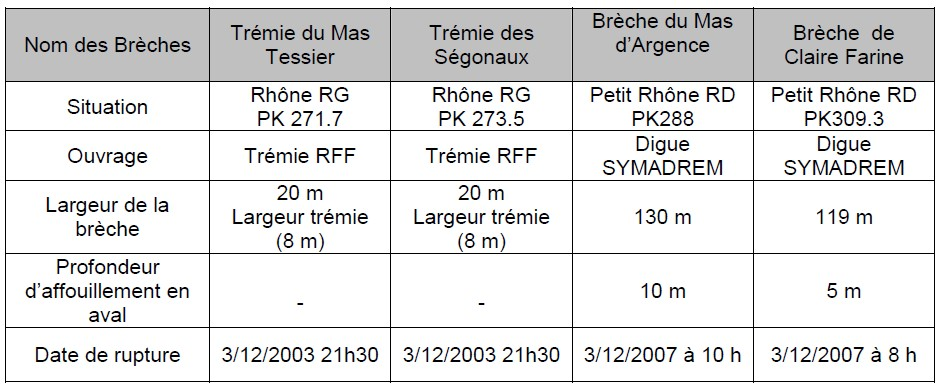
\includegraphics[width=.7\linewidth]{Figures/Breches2003.jpg}
        \caption{Caractéristiques des brèches dans les digues lors de la crue de décembre 2003, tiré de l'étude du \citet{symadrem_programme_2012}.}
		\label{fig:Breches2003}
	\end{figure}		
	
	\subsubsection{Sensibilité aux surcotes marines}	
	
	\paragraph{} Les surcotes marines sont fréquentes en Méditerranée lors de conditions météorologiques telles que les tempêtes ou les fortes dépressions. Dans de nombreux témoignages historiques, des crues du bas-Rhône sont associées à des tempêtes maritimes \citet{pichard_sept_2014}. Ces augmentations périodiques du niveau de la mer peuvent avoir une influence sur les niveaux d'eau du Rhône. Cet impact est étudié en augmentant artificiellement le niveau de la mer en condition limite aval du modèle pour le bief du Petit-Rhône. La limite aval pour le bief du Grand-Rhône, située à Arles, n'est pas modifiée dans ce scénario. On suppose une surcote marine centennale, estimée à +2 m par \citet{kergadallan_estimation_2015}. On constate dans la figure \ref{fig:Sensib4} que l'impact de la surcote est maximal au niveau de la mer et décroit vers l'amont. Il semble important sur le bief du Petit-Rhône, mais la différence de hauteur d'eau à Pont de Beaucaire de +0.2 cm. Cela représente une différence en débit de 23 m\textsuperscript{3}/s, soit une erreur d'environ 0.15\% d'après la courbe de tarage la plus récente élaborée au chapitre 3 REF. Suite à ce constat, il ne semble pas pertinent de considérer les surcotes marines pour la modélisation des crues historiques à Beaucaire. Cependant, ce scénario suppose que la hauteur d'eau en crue à Arles n'est pas impactée par la surcote marine, ce qui est peu probable. Ce scénario pourrait être plus amplement exploré en estimant un ordre de grandeur de la différence de hauteur d'eau engendrée à Arles dans le cas d'un événement de surcote marine observé par le passé. De plus, des simulations similaires pourraient être réalisées pour représenter l'impact des embâcles causées par des arbres ou des glaces flottantes comme cela est parfois le cas pour les crues historiques de la base HISTRHÔNE.
	\FloatBarrier
	\subsubsection{Conclusions sur la simplification du modèle}
	
	\paragraph{} Les quatre scénarios présentés précédemment représentent une analyse de sensibilité sommaire afin d'identifier l'impact de quelques hypothèses simplificatrices sur la ligne d'eau à Beaucaire pour un débit constant correspondant au débit de pointe de la crue centennale de décembre 2003. Il s'agit de réduire au maximum la complexité du modèle afin de le rendre utilisable pour la simulation de crues historiques pour lesquelles les données sont rares. Il faut noter que même si l'impact de chacune de ces hypothèses simplificatrices est relativement faible, l'impact cumulé de plusieurs d'entre elles peut en revanche être significatif. Par exemple, on peut imaginer le cas d'une crue pour laquelle des brèches dans les digues ont été observées mais dont la taille n'est pas connue, et pour laquelle une surcote marine d'une amplitude inconnue a été observée. D'autres facteurs engendrent une incertitude importante des débits modélisés mais ne sont pas inhérents à la simplification du modèle. On peut notamment penser aux effets d'hystérésis dont l'impact sur les stations hydrométriques françaises a été explorée par \cite{perret_framework_2022}, mais également à la complexité d'estimer des apports du Gardon ainsi que les phénomènes de laminages au niveau de la confluence \citep{symadrem_programme_2012}. Plus intuitivement, on aussi penser aux incertitudes liées à la reconstitution des géométries et des rugosités historiques.
	
	\subsection{Bathymétries et topographies anciennes}
	
	\paragraph{} Une des principales limites de la modélisation des crues anciennes provient de la reconstitution de la géométrie des sections en travers. Les nombreuses évolutions morphologiques de la basse vallée du Rhône décrites pour les deux derniers siècles par \citet{raccasi_mutations_2008}, et pour les sept derniers	par \citet{pichard_sept_2014}, incitent à la plus grande prudence. Ces évolutions semblent a minima impacter le lit mineur et le lit moyen. Les évolutions du lit majeur semblent en revanche limitées aux conditions d'occupation et aux aménagements de protection pour les plus fortes crues. Les données bathymétriques complètes les plus anciennes correspondent aux planches cartographiques du Rhône navigable de Lyon à la mer, provenant des archives \citet{cnr_cartes_1908}, dont les mesures ont été réalisées entre 1907 et 1908 pour la zone de Beaucaire (figure \ref{fig:BathyTopo}, haut). Les relevés bathymétriques sont calés sur la ligne d'eau d'étiage de 1907-1908. Seul le chenal de navigation est représenté, ce qui peut poser problème, notamment à Beaucaire où seule la bathymétrie du chenal navigable (en rive droite à cette époque) est représentée. Il est possible de reconstituer la bathymétrie des chenaux secondaires pour les quelques sections en travers où des relevés sont disponibles autour de 1845 (figure \ref{fig:ProfGoux}), soit avant les travaux de correction de Girardon, lancés dès 1860. En ce qui concerne le lit majeur, la carte topographique du cours du Rhône (1860) est un document exceptionnel provenant des archives \citet{cnr_carte_1876}, qui présente des relevés topographiques réalisés entre 1857 et 1876, avant la grande phase d'aménagement du fleuve. Les relevés de la zone de Beaucaire ont été réalisés entre 1870 et 1876 (figure \ref{fig:BathyTopo}, bas). Des profils transversaux sont disponibles tous les kilomètres (sous réserve de parvenir à les déchiffrer) et couvrent un profil allant des limites du lit mineur jusqu'au delà des limites du lit majeur.
		
	\begin{figure}[h]
		\centering
		\begin{subfigure}{.7\linewidth}
			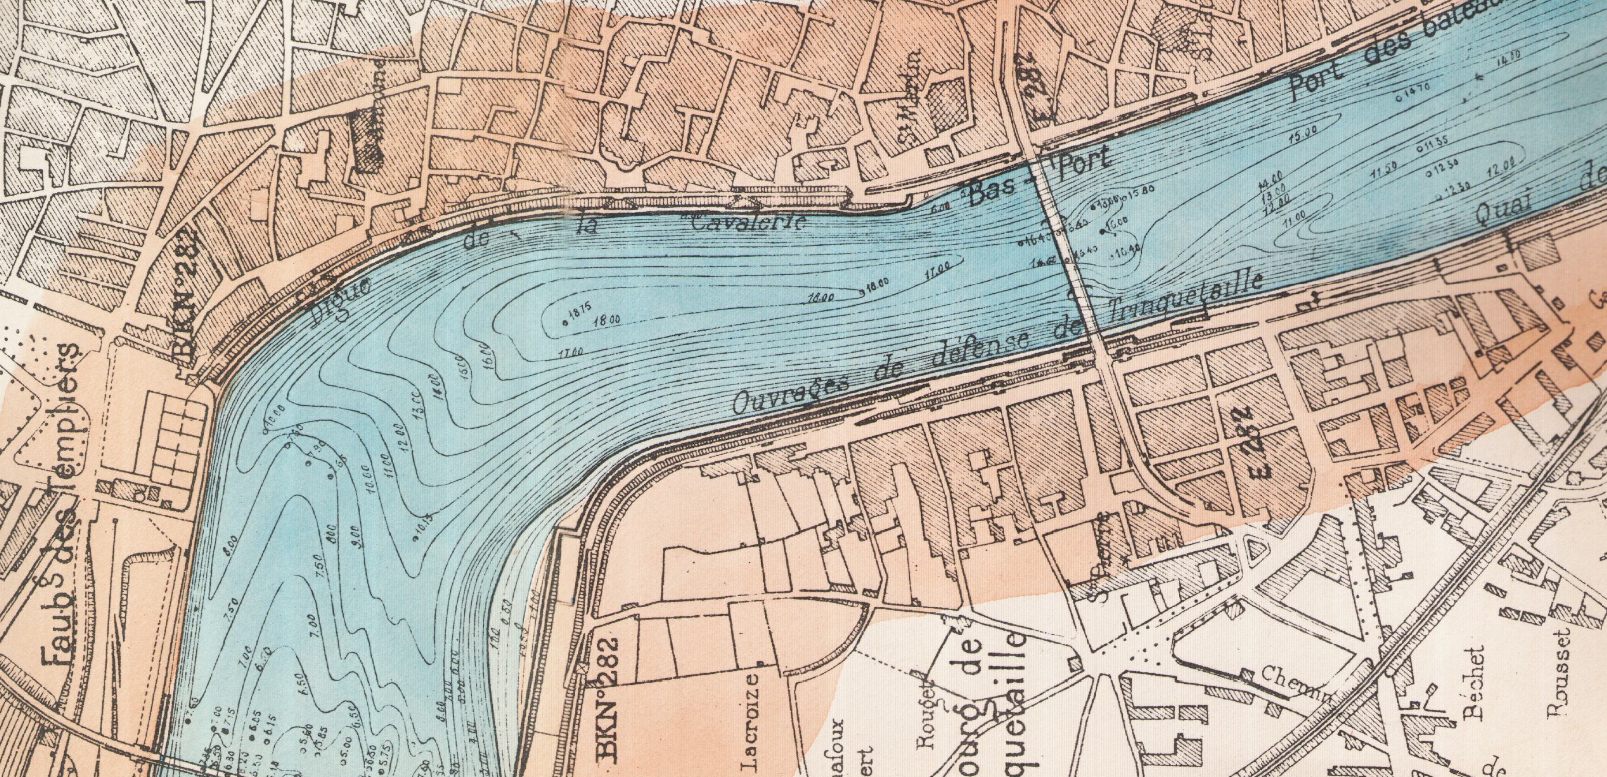
\includegraphics[width=\linewidth]{Figures/BathyArles1897.png}
		\end{subfigure}
		\begin{subfigure}{0.7\linewidth}
			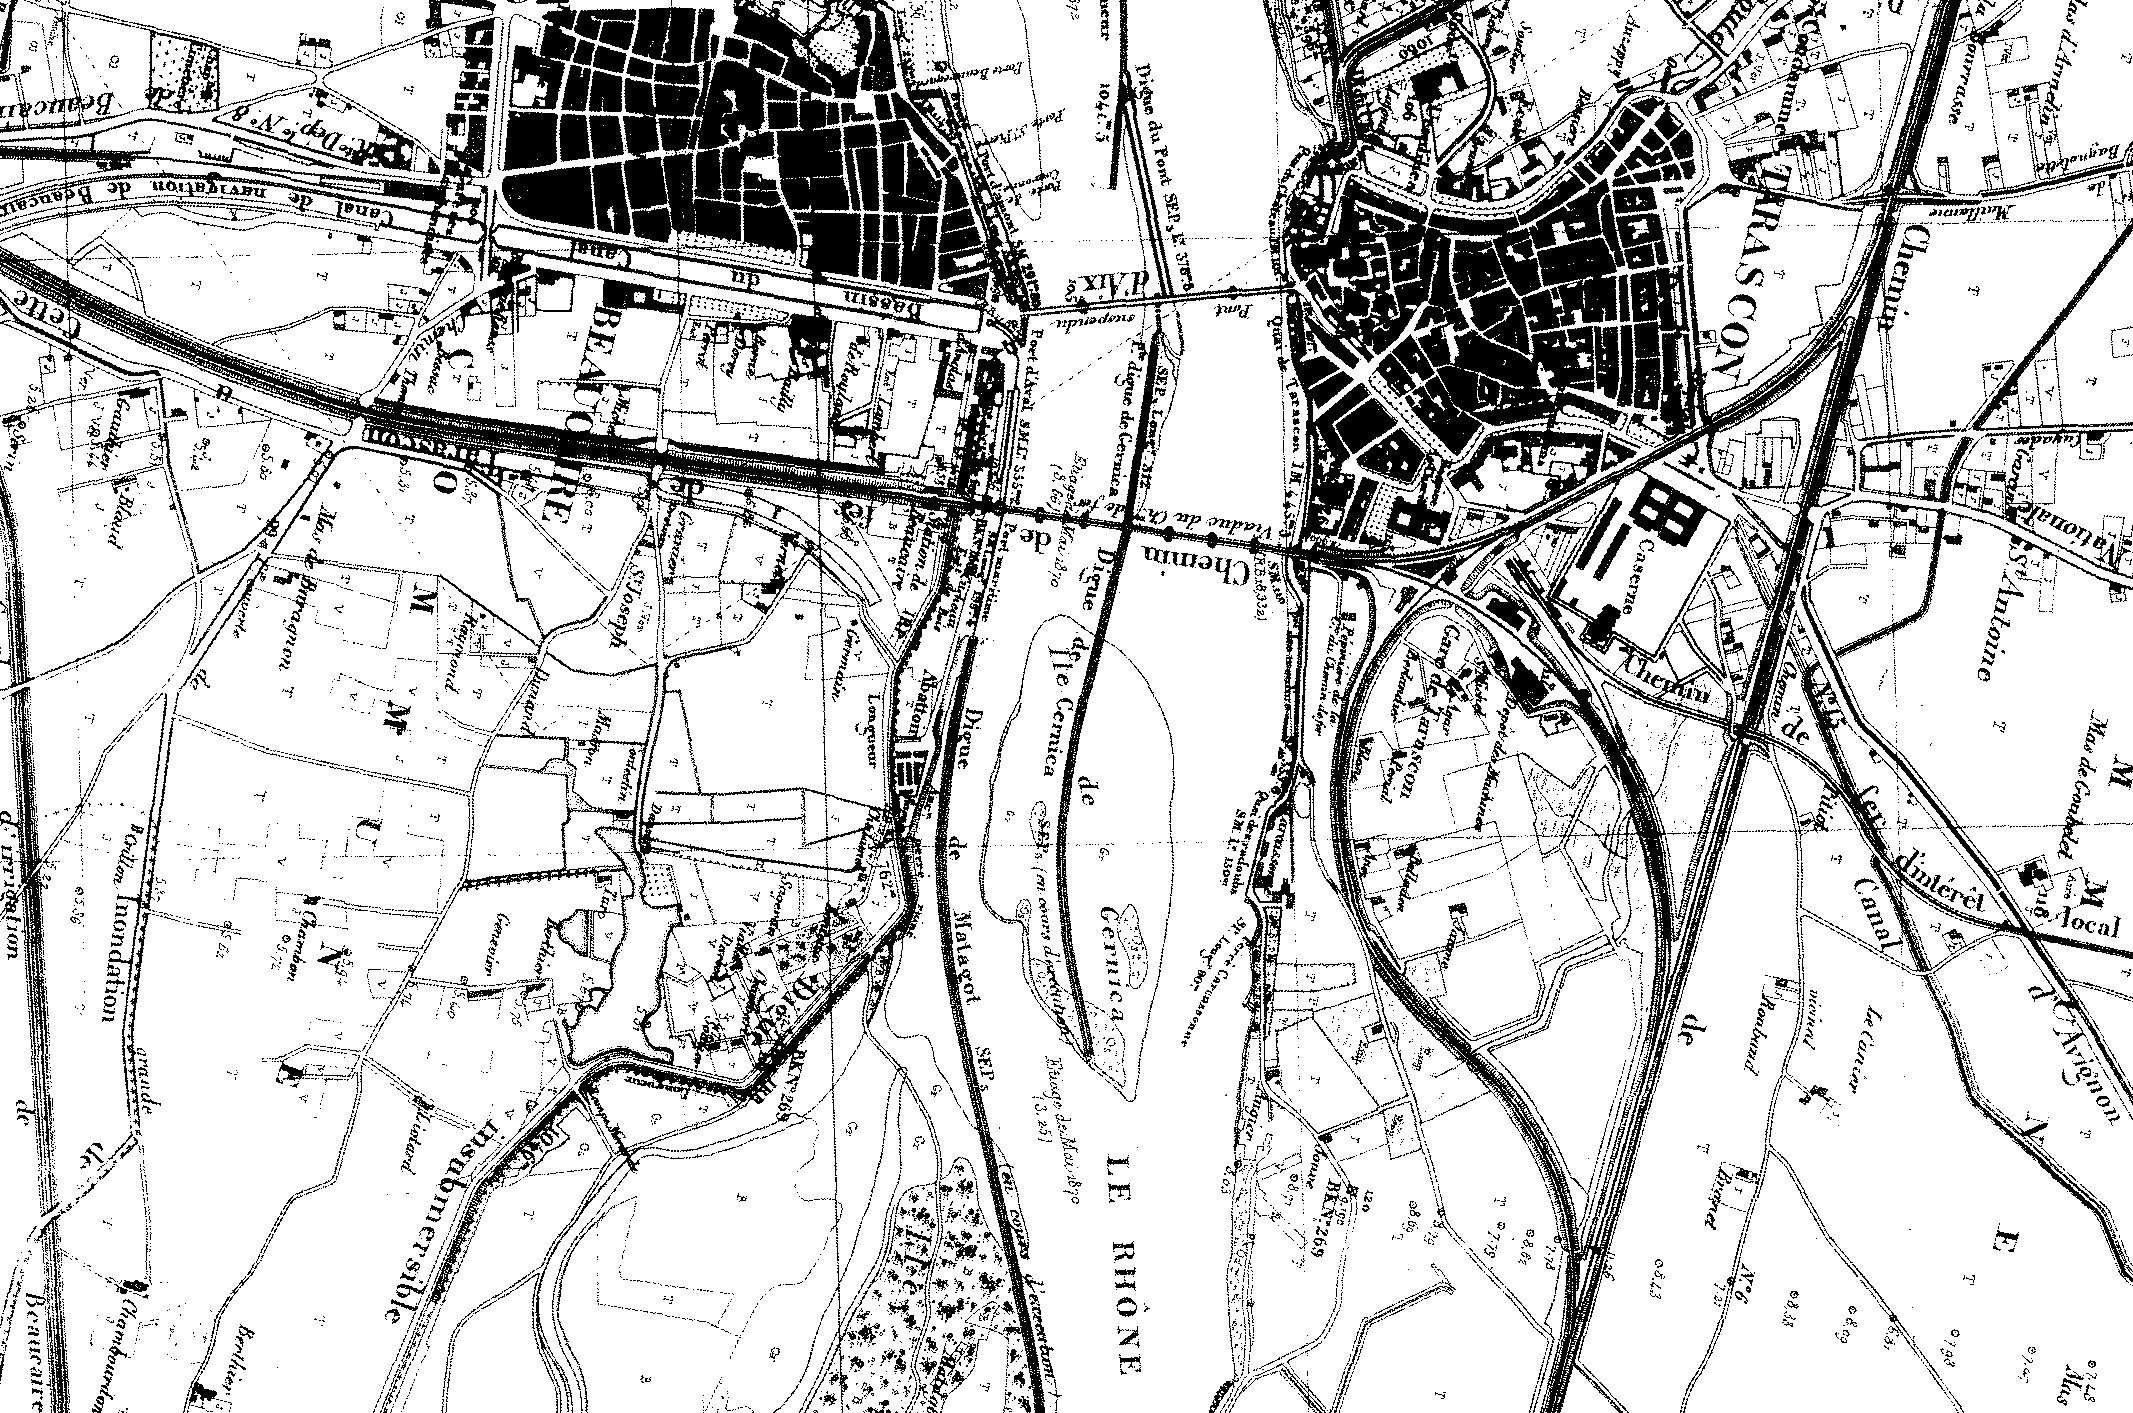
\includegraphics[width=\linewidth]{Figures/Atlas1860.jpg}
		\end{subfigure}
		\caption{Haut : Carte bathymétrique du Rhône de Lyon à la mer (1897-1908) pour la zone d'Arles \citep{cnr_cartes_1908}. Les isobathes sont données par rapport à l'étiage de 1908. Les relevés couvrent seulement le chenal navigable du Rhône. Bas : Carte topographique du cours du Rhône (1860), pour la zone de Beaucaire-Tarascon \citep{cnr_carte_1876}. Pour chaque point kilométrique, un profil en travers est disponible (points en bas à droite). Les altitudes sont dans le système de nivellement Bourdalouë.}
		\label{fig:BathyTopo}
	\end{figure}
	
	\paragraph{} En résumé, les plus anciennes données topographiques et bathymétriques disponibles en basse vallée du Rhône remontent au milieu du XIX\textsuperscript{ème} siècle. La modélisation des crues antérieures aux relevés limnimétriques (débutant en 1816) de la base HISTRHÔNE devra donc s'appuyer sur ces données faute de mieux. De fortes hypothèses quant à la morphologie du lit mineur (et dans une moindre mesure du lit majeur) devront être faites. Il sera par exemple possible de simuler un enfoncement ou un exhaussement de la totalité du lit majeur au sein du modèle. 
	
\FloatBarrier	
	
	\subsection{Recensement des informations nécessaires à la modélisation hydraulique} 
	
	\paragraph{} Des informations jugées utiles à la modélisation ont été extraites de la base HISTHRÔNE pour les crues de la catégorie C4 de 1353 à 1840. Elles sont présentées dans l'annexe \ref{sec:TabC4} REF sous la forme d'un tableau. Chacune des crues est succinctement décrite (zone inondée, causes probables, etc.) et les informations jugées nécessaires à la modélisation sont renseignées. Ces informations sont très diverses : réaction des affluents, hauteurs aux échelles reconstituées, mentions de hauteurs d'eau hors échelle limnimétrique, dégâts aux digues de protections, etc. Pour certaines crues, les informations disponibles semblent parfois suffisantes pour en estimer le débit via la modélisation hydraulique. Ce n'est pas toujours le cas. Ces divers niveaux d'information disponibles dans la base HISTRHÔNE sont explorés via les exemples suivants. 
	
	\paragraph{} L'inondation de 1745 est due à trois crues successives dont la première était la plus forte le 4 novembre. \textit{«Les pluyes abondantes et continuelles des 4,5,6,7 Novembre 1745 ayant inondé tout le terroir de cette ville et celui des villes voisines, la roubine du Vigueirat ne pouvant contenir ses eaux rompit et versa en divers quartiers de Trébon, les eaux du Rhône vinrent sur le quai, la chaussée du Trébon rompit à demi quart de lieue de la ville […]»} (source : Notes historiques sur Arles, BM Arles). La hauteur à l'échelle reconstituée de Véran à Arles est de 5.31 m et de nombreuses informations de hauteurs d'eau hors échelle sont également disponibles : \textit{«2.5 m d'eau dans les maisons de Tarascon où le Rhône entrait par la porte du château}»; \textit{«Tarascon est en partie sous 10 pieds [3,25 m] d'eau et il y a 10 à 12 pieds d'eau dans la plupart des maisons}»; \textit{«[3.5 m] d'eau sur le Pont de Crau»}. Les digues ont connu de nombreux dégâts qui sont rapportés avec précision : \textit{«Brèche de [60 m] de large à la chaussée du Trébon à [500 m] d'Arles»; «[600 m] d'ouvertures au pas du bouquet [Tarascon]»;«Rupture de la roubine du Vigueyrat [Arles]»;«Chaussée de Camargue rompue en plusieurs endroits du côté du Baron»;« Il semble que les premiers débordements proviennent du canal du Vigueirat, qui inonda le Trébon, avant la rupture des chaussées en ce même quartier, à un demi quart de lieue [environ 600 m] de la ville [probablement près de l'actuelle gare d’Arles]»}. De plus, on peut noter que \textit{«le rhone a diminué de 10 pieds d'un coup, certainement suite aux ruptures de digues à Tarascon»}. Ainsi, moyennant quelques hypothèses sur la hauteur des brèches faites aux digues de protection, il semble possible de modéliser le débit de cette crue à l'aide des nombreuses hauteurs d'eau disponibles aux échelles et en dehors. 

	\paragraph{} Dans d'autres cas, bien que des informations de hauteur d'eau soient disponibles, des brèches aux digues sont mentionnées à plusieurs reprises mais leur longueur n'est pas connue, ce qui peut compliquer l'estimation du débit. On peut par exemple citer le cas de la crue de décembre 1755 qui est décrite comme étant la crue la plus importante du XVIII\textsuperscript{ème} siècle. La crue atteint 5.47 m à l'échelle Véran d'Arles. Des hauteurs hors échelle sont également disponibles : 2.6 m dans la plaine de Beaucaire; 2 m d'eau dans les maisons du quartier Notre Dame de Bonne Aventure à Tarascon; 2.75 m dans les maisons à coté de la porte St Jean; etc. Cependant, les informations concernant les brèches sont sporadiques : \textit{« Brèche à la chaussée d'Argence, les eaux remontent jusqu'à environ 12 km dans le terroir »}. L'estimation d'un débit dans ces conditions est donc relativement incertaine.
  	
	\paragraph{} Enfin, d'autres crues semblent complètement inexploitables, en l'absence de données de hauteur fiables. Par exemple, pour la crue dite «\textit{extraordinaire}» de 1573, aucune hauteur n'est disponible, que ce soit aux échelles reconstituée ou en dehors. En revanche de nombreuses ruptures de digues sont mentionnées : \textit{«Vers Beaucaire, plus de [6 km] de chaussées ruinées. Dont 25 cannes à la Bergantière, 500 cannes au dessus du port ne autre au trou du Sauze »}. 
	
	\paragraph{} On peut également relever des cas très particuliers, comme la crue de 1674, initiée par la Durance les 15 et 16 novembre. Au cours de cet événement, \textit{«les eaux de la Durance se jettent en partie dans le Trébon par le débouché de Saint-Gabriel »} (près de Tarascon). Cette avulsion représente un changement morphologique majeur. La modélisation du débit de cet événement en l'absence de données plus précises que des seuls témoignages semble dans ce cas inespérée.	
	
	\paragraph{} Suite à cet état des lieux, il semble complexe de pouvoir modéliser le débit de chacune des crues C4 de la base avec un même modèle hydraulique. De plus on constate de grandes disparités entre les informations disponibles d'une crue à l'autre, ainsi que des changements morphologiques majeurs pour certains événements. Chacune des crues mériterait une analyse détaillée ainsi qu'une adaptation du modèle hydraulique. Aussi, d'importantes incertitudes semblent entourer cet exercice. Il faut également noter que dans ce contexte, la quantification des incertitudes de modélisation semble particulièrement complexe. La question de la faisabilité de ces reconstitutions devant le temps limité de la thèse s'est donc posée. La plus value de ces estimations de débit semble faible alors que cet exercice est très chronophage et incertain. Sachant qu'il est possible d'intégrer ces événements à l'analyse fréquentielle des crues en utilisant la seule information du nombre de dépassements d'un seuil de perception, la modélisation hydraulique du débit des crues C4 est abandonnée. En revanche, les événements historiques présentés ci-dessus et dans l'annexe \ref{sec:TabC4} seront utilisés sous forme d'occurrences supérieures à un seuil de perception. 
	
	\epigraph{"\textit{Je ne dirais pas que c'est un échec. Ça n'a pas marché.}"}{Emmanuel Macron le 14 octobre 2020}
		
	\FloatBarrier	
	\subsection{Limites et perspectives pour la modélisation hydraulique des événements historiques}
	
	\paragraph{} Les travaux décrits dans cette section n'ont pas permis, dans le temps limité de la thèse, d'estimer le débit des événements anciens à l'aide de la modélisation hydraulique. Cependant, ils ont permis de dresser un bilan des données disponibles à cet effet, ainsi que d'en identifier les limites. L'impact de plusieurs hypothèses permettant une simplification du modèle hydraulique a également été exploré dans le but de pouvoir effectuer des modélisations avec une quantité minimale de données d'entrée. Les idées développées dans les lignes suivantes ont pour but de définir les contours et les limites à garder en tête dans l'optique de poursuivre ce travail d'estimation du débit des événements historiques à Beaucaire.
	
	\paragraph{} Pour commencer, la limite amont du modèle a été définie à l'aval immédiat de la confluence avec la Durance, ce qui permet d'éviter l'estimation du débit de cet affluent. Cependant, il reste à définir une solution pour la confluence du Gardon. Dans le modèle présenté dans cette section, celui-ci était représenté par un apport latéral, mais l'estimation du débit de cet apport est impossible dans le cas d'événements historiques. Une des possibilités pour contourner ce problème serait de fixer la limite amont du modèle à l'aval immédiat de la confluence avec le Gardon. Il faut garder à l'esprit que la morphologie historique de cette confluence est plus simple que la morphologie actuelle, le Gardon se jetant dans le Vieux-Rhône et n'ayant pas d'influence sur le débit du chenal de dérivation. Ensuite, la reproduction dans le modèle des deux chenaux présents à Beaucaire (qui communiquent à haut débit) est un obstacle conséquent pour la modélisation 1D car il est complexe de modéliser leur communication à haut débit. Seule la modélisation 2D peut permettre de reproduire ce phénomène de manière convenable, mais elle nécessite une quantité d'informations plus importante. Il semble donc nécessaire, dans un but de simplification, de fixer la limite amont du modèle à l'amont de la division du Rhône en deux bras. 
	
	\paragraph{} En ce qui concerne la limite aval, la conservation du Petit-Rhône jusqu'à la mer dans son état actuel semble être la solution la plus évidente et la moins couteuse en terme de données pour garantir une extraction cohérente des débits du Rhône. La limite aval du Grand-Rhône fixée à Arles semble également être la meilleure solution compte tenu des niveaux reconstitués par Véran à l'échelle du port \citep{pichard_les_1995}. Pour 10 des 18 crues C4 de 1300 à 1810, une estimation de la hauteur à Arles est disponible (voir Annexe \ref{sec:TabC4}). La modélisation semble en revanche plus complexe pour les 8 autres crues, pour lesquelles la limite aval pourra par exemple être fixée au niveau de la mer, des reconstitutions historiques du niveau marin étant probablement disponibles.
	
	\paragraph{} En ce qui concerne la géométrie du Rhône en entrée du modèle, les données topographiques et bathymétriques disponibles ne permettent pas de remonter à une époque plus ancienne que le milieu du XIX\textsuperscript{ème} siècle. Les conditions d'écoulement pré-1816 sont méconnues bien que des cartes anciennes et assez approximatives existent (par exemple, la carte de Bompar datant de la fin du XVI\textsuperscript{ème} siècle). Il s'agit par exemple de la carte de Cassini datant du XVIII\textsuperscript{ème} siècles ou des cartes présentées par \citet{pichard_sept_2014}. Des hypothèses grossières pourront être faites sur les bathymétriques des périodes anciennes, par exemple en exhaussant ou en enfonçant artificiellement le lit mineur dans le modèle hydraulique, suivant les constatations de \citet{pichard_sept_2014} ou d'autres études de la géomorphologie ancienne du Rhône. Cette méconnaissance de la morphologie du Rhône avant 1800 est la plus grosse inconnue autour des reconstitutions des débits anciens.
	
	\paragraph{} Dans les premiers essais de modélisation présentés dans ce chapitre, le calage de la rugosité du chenal du modèle OSR a été conservé, bien que celui-ci ne soit pas adapté à un contexte de crue. Ce calage pourrait être revu, une fois les profils en travers du modèle revus sur la base des topographies et bathymétries du XIX\textsuperscript{ème} siècle. La reproduction de la crue de 1856 pourrait être une première étape de ce calage, des lignes d'eau de cet événement étant disponibles dans les archives CNR. Cependant, les coefficients de rugosité de 1856 ne sont probablement pas valables pour les crues antérieures au XIX\textsuperscript{ème} siècle. Il semble complexe d'adapter ces coefficients sur la base de l'occupation des sols pré-XIX\textsuperscript{ème} siècle, les données cartographiques de cette période étant rares et imprécises. 
	
	\paragraph{} En résumé, de nombreuses incertitudes entourent l'estimation du débit des crues anciennes. Ces incertitudes proviennent notamment des données d'entrée, mais également du modèle lui-même qui représente une représentation très simplifiée de la réalité des écoulements historiques. Voici une liste non exhaustive de ces différentes incertitudes :
	
	\begin{itemize}
		\item La reconstitution imprécise des sections en travers historiques du Rhône, basée sur des bathymétries plus récentes (XIX\textsuperscript{ème} siècle) que les crues de la base HISTRHÔNE.
		\item L'incertitude des niveaux exacts atteints par les crues que les témoignages anciens ne reflètent pas parfaitement. En effet, de nombreuses informations sur les zones impactées par les crues sont disponibles, mais celles-ci ne mentionnent que rarement la profondeur maximale atteinte.
		\item  L'existence de brèches dans les digues qui, bien que souvent mentionnées dans les écrits, ne permettent pas de reconstituer la largeur et la profondeur de ces brèches, ainsi que leur évolution au cours de la crue.
		\item L'incertitude autour de la dynamique de la crue qu'il est impossible de connaitre en l'absence de mesures continues.
		\item La connaissance imparfaite des conditions aux limites du modèle, tel que le niveau de la mer Méditerranée pour le bief du Petit-Rhône, qu'il est impossible de connaitre pour les crues du XIV\textsuperscript{ème} siècle.
		\item Les coefficients de rugosité du modèle, qu'il est complexe d'estimer compte tenu de la méconnaissance de l'occupation des sols et de leur nature pour les périodes anciennes.	
	\end{itemize}
		
	\paragraph{} La quantification de l'incertitude des débits estimés est nécessaire mais semble complexe. Elle pourra par exemple passer par des hypothèses hautes et basses sur les différents points listés ci-dessus. Un autre moyen plus complexe et couteux en temps de calcul consiste à élaborer un algorithme Monte Carlo couplé au modèle hydraulique permettant de propager l'ensemble des incertitudes au résultat final.	
	

\FloatBarrier
\section{Conclusion du chapitre}

	\paragraph{} Une chronique limnimétrique continue exceptionnellement longue (205 années entre 1816 et 2020) est disponible à Beaucaire. La station de Beaucaire est d'une grande importance car elle est la station du Rhône "complet" la plus à l'aval du bassin versant. Elle enregistre donc la grande complexité des très divers apports du Rhône. L'échelle limnimétrique du Pont de Beaucaire n'a supposément jamais été déplacée depuis son installation en 1816. Elle fut donc le témoin des nombreux changements naturels et anthropiques du chenal : des digues de protection contre les inondations, jusqu'aux aménagements en lit mineur pour favoriser la navigation, en passant par l'installation d'aménagements hydroélectriques. L'installation de ces derniers en 1970 a nécessité le déplacement de la station quelques centaines de mètres plus à l'aval. Ce riche historique limnimétrique peut permettre la reconstitution d'une chronique de débits de plus de deux siècles, à condition de prendre en compte les nombreuses évolutions du chenal compilées dans ce chapitre lors de l'élaboration des courbes de tarage. De plus, à l'image des travaux de \citet{bard_actualisation_2018}, une prise en compte des nombreuses sources d'incertitude sera nécessaire. 
	
	\paragraph{} La reconstitution de deux siècles de débit en continu semble envisageable suite au bilan des données hydrométriques disponibles. Cependant, il faudra veiller à l'homogénéité de la chronique reconstituée. Contrairement à certains fleuves européens, le Rhône n'a pas connu de dérivations ou de travaux majeurs, mis à part le canal de Savières près de Chambéry, avec un impact négligeable à Beaucaire. Cependant, plusieurs autres facteurs peuvent impacter cette homogénéité, et notamment l'installation d'aménagements en lit mineur qui peuvent modifier la dynamique des crues. Afin de quantifier cet impact, l'évolution du temps de propagation des crues au fil de l'installation des différents aménagements en lit mineur a été étudiée. Les temps de propagation entre Lyon et Beaucaire de 121 crues non-débordantes de type océanique ont été compilés suite à l'analyse des limnigrammes. Il apparait que le temps de propagation de ce type de crues a progressivement diminué au cours des différentes phases d'aménagement et est passé d'environ 48 h en 1840 à environ 16 h de nos jours. La modélisation hydraulique d'un événement océanique type dans le contexte actuel à permis d'obtenir un temps de propagation de 18 h, ce qui confirme la valeur de 18 h estimée à l'aide des limnigramme. Les aménagements en lit mineur ont probablement d'autres conséquences, notamment sur la forme des hydrogrammes de crue, le débit de pointe, ou la concomitance des crues du Rhône avec celles de ses affluents. Ces évolutions devront êtres gardées à l'esprit lors de l'évaluation de l'homogénéité des échantillons de crues préalables à l'analyse fréquentielle lors des chapitres suivants. L'impact de ces aménagements sur les temps de propagation de crues plus importantes, ou dans le cas de crues cévenoles ou généralisées n'a pas été étudié ici mais pourrait également être intéressant.
	
	\paragraph{} En plus du riche passé en terme de relevés limnimétriques, la basse vallée du Rhône, par son histoire religieuse et culturelle, regorge de documents qui témoignent de son histoire hydroclimatique. Ces éléments historiques ont été récoltés et mis à disposition dans la base de données HISTHRÔNE (\url{histrhone.cerege.fr}) à la faveur d'un très important travail d'archives \citep{pichard_sept_2014}. Ce sont ainsi plus de 1500 événements depuis le XIII\textsuperscript{ème} siècle que décrivent ces divers documents et témoignages. Les crues étant des événements marquants pour les populations ripariennes, elles sont nombreuses dans la base de données, où elles sont classées selon les dommages engendrés. Une estimation de l'ordre de grandeur du débit de ces catégories a été effectuée en se basant sur une comparaison des crues récentes avec les hydrogrammes de Beaucaire. Ces estimations pourront permettre l'utilisation des crues antérieures aux enregistrements continus pour l'analyse fréquentielle à condition de considérer un seuil de perception dont le débit n'est pas parfaitement connu. De plus, des probables fluctuations de la vulnérabilité des populations aux inondations ont été mises en évidence et peuvent compliquer l'utilisation des seules mentions de crues pour l'analyse fréquentielle en l'absence d'estimations de débit pour chacun des événements. 

	\paragraph{} La piste de la modélisation hydraulique pour l'estimation du débit des crues historiques a été explorée. Le modèle MAGE OSR 1D utilisé pour étudier la dynamique sédimentaire du Rhône du Lac Léman à la mer a été adapté à l'étude des crues du bas Rhône. Étant donné la complexité de reconstituer la morphologie et la bathymétrie du Rhône avant le XIX\textsuperscript{ème} siècle, la sensibilité du modèle à plusieurs hypothèses simplificatrices a été explorée afin d'en réduire la complexité. Il apparait notamment de ces tests que la meilleure configuration semble être de considérer comme limite aval du modèle côté Grand-Rhône la ville d'Arles, où la hauteur d'eau de nombreuses crues historiques est disponible \citep{pichard_hauteurs_2013}. La fixation de la limite aval du Petit-Rhône à son embouchure semble être la solution la plus pratique en l'absence d'enregistrements de hauteur des crues historiques sur ce bief. Il sera cependant complexe de reconstituer la bathymétrie de ce bief dont la morphologie a grandement évolué au cours de l'histoire. Par la suite, l'impact de différents scénarios sur la ligne d'eau à Beaucaire a été exploré : la présence d'aménagements hydroélectriques, la présence de brèches dans les digues du Petit-Rhône (scénario de la crue de 2003), l'évolution morphologique du Petit-Rhône (et l'hypothèse extrême de sa suppression du modèle), la présence d'une surcote marine pendant la crue. Il apparait que parmi ces quatre scénarios, seule la considération des aménagements hydroélectriques a un impact significatif sur la ligne d'eau à Beaucaire. Cependant, des perturbations apparaissant dans des zones plus proches de la station de Beaucaire n'ont pas été modélisées mais pourraient avoir un impact plus important.
	
	\paragraph{}	 Au-delà de ces différents scénarios de simplification du modèle, plusieurs limites à la reconstitution du débit des crues anciennes persistent et ont été listées. La principale limite étant la reconstitution des sections en travers du Rhône et de leur rugosité avant le XIX\textsuperscript{ème} siècle. En effet, les plus anciennes données disponibles ne remontant qu'en 1908 pour la bathymétrie et en 1876 pour la topographie de la plaine alluviale. De plus, l'estimation de l'incertitude autour des débits modélisés semble également complexe à réaliser. Au regard du temps limité de la thèse et la possibilité d'utiliser ces données historiques pour l'analyse fréquentielle des crues sans avoir à en modéliser le débit via l'estimation d'un seuil de perception, nous avons décidé de ne pas poursuivre ces travaux. Cependant, les contours et les limites de cet exercice ont été définis, ce qui pourra être utile à qui envisagera de telles reconstitutions. 
	
	
%	\paragraph{} Le présent chapitre a permis de dresser le bilan des données de crues disponibles à Beaucaire. Tout d'abord, une chronique limnimétrique continue de 1816 à aujourd'hui est disponible, permettant l'estimation des débits de cette période via l'élaboration de courbes de tarage. L'analyse de l'évolution de la morphologie du Rhône au cours des deux derniers siècles sera utile à cet effet. Il faudra cependant porter une attention particulière à l'estimation et la propagation des diverses incertitudes provenant de la mesure de hauteur d'eau, des jaugeages, ou de l'élaboration des courbes de tarage. Les données de la base HISTRHÔNE ont ensuite permis de rassembler un nombre important d'événements de crues antérieurs à l'installation de l'échelle limnimétrique de Beaucaire (1816). Ces crues sont classées dans la base de données en différentes catégories selon les dommages engendrés. Il faudra garder à l'esprit que la vulnérabilité des populations aux crues du Rhône à pu changer au cours de l'histoire et impacter la classification des événements. Si le débit des événements anciens n'a pas pu être estimé à l'aide de la modélisation hydraulique, les limites et les contours de cet exercice ont pu être définis. Il faut garder à l'esprit que l'utilisation des données pré-enregistrements continus pour l'analyse fréquentielle des crues n'est pas conditionnée à l'estimation du débit de chacun des événements. Pour finir, l'évolution du temps de propagation des crues au cours des différentes phases d'aménagements en lit mineur a été étudiée. Il faudra s'assurer que la diminution du temps de propagation des crues mise en valeur dans ce chapitre n'a pas d'impact sur l'homogénéité des échantillons utilisés pour l'analyse fréquentielle. 

\newpage

\section{Annexe 1 : Données des crues C4 de la base HISTRHÔNE pour la modélisation hydraulique}
\label{sec:TabC4}
%
%\begin{tiny}
%
%\begin{landscape}
%	\begin{longtable}{|p{0.4cm}|p{0.5cm}
%	 |p{0.5cm}|p{2cm}|p{0.5cm}|p{2cm}|p{1cm}|p{1cm}|p{1cm}|p{1cm}|p{1cm}|p{1cm}|p{2cm}|p{1cm}|}
%	
%    \hline
%  \textbf{Année} & \textbf{Mois} & \textbf{Modélisable } & \textbf{Description} & \textbf{Causes} & \textbf{Info affluents} & \textbf{Hauteurs échelle} & \textbf{Info hauteur Beaucaire - Tarascon} & \textbf{Info hauteur Arles} & \textbf{Info hauteur Avignon} & \textbf{Indices hauteur autre} & \textbf{Ouverture digues} & \textbf{Autres infos} \\ \hline
%        \textbf{1353} & mai & Non & Le Rhône inonde la plaine depuis Avignon jusqu’à la mer. & Gel du Rhône et de la Durance & ~ & ~ & ~ & ~ & ~ & x & ~ & ~ \\ \hline
%        \textbf{1398} & octobre & Non & Crue dévastatrice du Rhône selon les chroniques d'Avignon et de l'arlésien Bertran Boysset & ~ & ~ & ~ & ~ & ~ & ~ & inférieur de 10 cm à la crue de 1396 à Arles (qui est une C3?...) & ~ & ~ \\ \hline
%        \textbf{1433} & novembre & Oui (Avignon) & Grande inondation qui s'étend d'Avignon à la mer & Pluie et fonte des neiges (en novembre?) & Débordement conjoint Durance et Sorgue & 6,77 m au dessus de l'étiage à Avignon, échelle indéterminée et 7,08 m au pont suspendu d'Avignon & ~ & ~ & Miracle chapelle des pénitents gris, 1 m d'eau dans la nef & ~ & ~ & Toute la Carmarque est inondée, des pirates y pénètrent et se livrent à des pillages \\ \hline
%        \textbf{1471} & septembre & Non & L'une des plus grandes inondations conjuguées du Rhône et de la Durance & Probablement cévenol, caractère brutal & Durance en crue & X & ~ & ~ & une partie des murailles abattues, repère de crue église st michel de Caderousse, 1m52 au dessus du dallage & Caderousse, chapelle d'Ancezune, 1m52 au dessus du dallage & à Arles & ~ \\ \hline
%        \textbf{1529} & novembre & Oui & "Grande inondation du Rhône dit de Saint-Martin (""La Ronada de San Martin"") à Arles." & X & X & 5,25 sur l'échelle de Véran (Arles) & porte St Jean de Tarascon endommagée par la crue & Trébon, plan du bourg et camarque inondés & 300 m de remparts abattus & ~ & Levées de la chaussée du trébon endommagée (arles) & ~ \\ \hline
%        \textbf{1548} & novembre & Oui (Avignon) & Caractère foudroyant à Avignon mais peu d'échos à Beaucaire et Arles & crue à prépondérance océanique très nette, mais avec des apports duranciens et cévenols évoquant aussi des pluies méditerranéennes, limitées à un secteur étroit autour du couloir rhodanien & Débordement de la Durance à Avignon & X & Chaussées ruinées à Tarascon, murailles démolies & Hôpital St Lazare endommagé & " L'eau entre dans la ville ""jusques à la Saunerie, à Saint-Agricol, à la Croix de Lunel, à Sainte-Catherine … HR.   L'eau atteint la coquille de la chapelle St Nicolas sur le pont St benezet,   25 cm en dessous du plus haut de la porte de la Ligne,   tient toutes les arcades du pont et à environ 1m50 avant de toucher le plus haut des arcs. RAPPORT COMPLET à revoir sur des contradictions concernant les marques de crues à Avignon" & nombreux indices contradictoires à Avignon quand au dépassement par cette crue de celle de 1856. & ~ & ~ \\ \hline
%        \textbf{1570} & décembre & Hauteur seulement & Inondation générale du Rhône, concernant l'ensemble du bassin. Inondation extraordinaire commençant à Lyon le 2 décembre 1570 et qui atteint Avignon le 5 décembre, et emporte ensuite les chaussées d'Arles. & Pluies océaniques + fonte des neiges suite à un réchauffement brutal & X & 5,17 sur l'échelle de Véran à Arles & Le Rhône déborda de telle sorte qu'il tenoit toute la Camargue, les plans de St Gilles, Bellegarde, jusques à Beaucaire Tresbons et le Plan du Bourg & Chaussées emportées & Quartiers bas de la ville inondés & ~ & ~ & Lyon inondé, maisons détruites à la Guillotière \\ \hline
%        \textbf{1573} & octobre & Oui & "Inondation ""extraordinaire"" du Rhône à laquelle on peut attribuer l'ouverture du Grau du Roi à Aigues-Mortes" & ~ & X & X & L'eau passe par-dessus les chaussées,principalemnt à la pauze St Martin. Tout le plat pays et terroire de Beaucaire est en eau, jusqu'aux abords de la montagne.  & X & Deux arches du pont d'avignon emportées & moins haute que celle de 1548 de 4 doigts à Caderousse. Tout Caderousse est sous l'eau sauf vers l'église et la place & "Vers Beaucaire, plus de 6km de chaussées ruinées. Dont 25 cannes à la Bergantière, 500 cannes au dessus du port (de St Gilles)  une autre au trou du Sauze. à St Gilles, la crue ne cause pas tant de tord qu'à Beaucaire car le torrent de Rebayres nettoie la grande robine qu'ils tiennent ouvert afin de vidanger le terroir. Les travaux sont urgents car le Rhône menace d'inonder l'ensemble du terroir jusqu'à l'étang de Maugio. à tarascon :  Grande chaussée endommagée et rompue en plus de 10 ou 12 endroits ""tant dessus que dessous de la présente ville""" & Ouverture du Grau du Roi \\ \hline
%        \textbf{1580} & août & Oui (Avignon) & "Le ""déluge"" n'aurait duré qu'un jour, soit il fut d'une intensité hors de toute norme, soit il intervenait sur des sols déjà détrempés, mais la période ne penche guère vers cette hypothèse. On doit donc davantage penser à une crue cévenole." & Pluies épouvantables du 24 août (Selon M Villard) & La Durance resta calme & X & ~ & Un ane trouvé sur le toit d'une maison ( mas de l'Ase) & L'eau dépasse et renverse le mur que soutient la coquille de la chapelle (Saint-Nicolas) du pont Saint-Bénezet. 6 pans d'eau à la place devant la croix. 60 maisons tombées à Caderosuse. L'eau rompit une porte du portal St Lazare & mur de soutien de la chapelle du pont d'avignon renversé & Beaucaire : Chaussées démolies en 4 endroits : les Saussan, au Radeau et deux endroicts du Coussac, ainsi qu'à la pauze St martin. A Arles : Tresbon , plan du bourg, corrèges et montlong, grande quantité d'ouvertures aux chaussées. & ~ \\ \hline
%        \textbf{1674} & novembre & Oui, QUID de la Durance qui se jette en partie dans le Rhône au niveau d'Arles? & La plus grave inondation rhodanienne survenue au XVIIe siècle avec important apport de la Durance. Toute la basse Provence et tout le bas Languedoc sont touchés. & 15 jours de pluie abondante et fonte des neiges (déjà?) & Très grande crue de la Durance les 15 et 16 novembre avec débordement à Avignon. Les eaux de la Durance se jettent en partie dans le Trébon par le débouché de Saint-Gabrieln (près de Tarascon). Débordement dévastateur de la Sorgue le 15 novembre (Sorgues), Drac et Romanche en crue, donc isère ? & 6,55 Pt susp Avignon, 6,38 Madone Avignon, 5,39 à Arles (Véran) & 1,50 m d'eau dans tout Tarascon, pont beaucaire tarascon emporté, digues brisées, chaussées détruites… 8 ou 9 pans d'eau devant la maison de ville de Tarascon & 2m dans l'église St Lazare d'Arles, 3m sur le pont de Crau &  de l'eau jusqu'à la barbe de la statue de saint françois (?) à Avignon, 2m40 dans le cloitre des minimes, 0,80 au dessous de la crue de 1755. Repère placé rue st michel sur l'église des célestins. Porte St lazare enfoncée & ~ & Chaussées du Trébon, plan du bourg, Roque de l'acier près de Tarascon, Lansac, et de l'isle de Camargue emportées. Toutes les chaussées de boulbon jusquà Tarascon renversées en raison de l'avulsion de la Durance vers Arles par le Vigueirat. Nombreuses ruptures à Beaucaires(toutes décrites dans la transcription) & Fort transport solide qui comble en partie le lit de la Durance, d'où son avulsion \\ \hline
%        \textbf{1694} & novembre & Oui & "Les eaux surmontent les chaussées et se répandent avec une rapidité prodigieuse dans tout le terroir depuis Saint-Gabriel à la mer : ""on allait par bateaux de Tarascon jusques à la mer, que l'isle de Camargues était également couverte d'eau et qu'on allait aussi d'Arles à Maguelone, en Languedoc, par bateaux à travers les champs.""" & pluies soudaines et vent de mer & Débordement de la Durance à Avignon & 4,95m échelle Véran d'Arles & 3 pieds d'eau dans le jardin des capucins de Tarascon mais pas d'eau dans le bas du couvant. Plan du bourg et trébon inondés. L'eau s'étend de la ville au ténément de Beynes.  & Le rhône entre dans la ville par la porte de Rousset et autres endroits le long du quai. Chaussée de Fourque rompue, l'eau se répand violemment dans toute la Camargue & Crue égale à 1679 à Avignon & 4,95 m Véran (arles) & Arles : 870 cannes de chaussées ouvertes [1 740 mètres] : au-devant du port de Fourques, au Clot Négadier et le long du grand Rhône (Rougnouse, Montlong, ...) et une quinzaine d'autres endroits (au-dessous d'Albaron, ...), ainsi que les chaussées des terres de la Porcelette, du Grand Passon et de Gouine, d'environ100 mètres. Beaucaire : 400 m de chaussés à la Lèque & beaucoup de sable partout sur le territoire à partir de beaucaire. Ponts de bateaux de Beaucaire et Arles rompus. Le vent de mer ramène des vagues jusque 3 lieues dans la terre ferme. On va d'Arles à Montpellier en bateau à travers champs \\ \hline
%        \textbf{1705} & novembre et Janvier suivant & Oui & "Le Rhône devient ""furieusement gros"" suite aux pluies." & une semaine de pluie continue & Durance et Verdon en crue & 5,03 à Arles (Véran) & ~ & 65 cm plus haut que 1647, de l'eau 50 cm au dessus de la grande chausée du Trébon, 2m d'eau sur le chemin du pont de Crau, 1,50m dans le quartier du Plan de Bourg, 1,3m partout depuis le pont de Crau jusqu'au bois des Cays, L'eau de la durance ayant déversé depuis chateaurenard arrive à arles via les terroirs.  & plus  d'1,25m d'eau dans les terres de Barbantane & 5,03 m Véran (Arles) & 300 m de chaussées détruites sur le terroir de Tarascon (infos plutôt précises sur la hauteur et largeur de chaque ouverture dans la transcription). Ouvertures faites lors de la première inondations élargies lors de la seconde.   & sable et limon dans les plaines \\ \hline
%        \textbf{1706} & Janvier & Oui, commun avec la précédente & "La récurrence de janvier 1706 achève de ruiner les pays riverains du Rhône et de la Durance. Inondation généralisée : ""les terroirs ressemblent à une mer. """ & pluies abondantes et prolongées & "Débordement de toutes les rivières en haute et basse Provence (Bassins de la Durance, du Verdon, de la Bléone, de l'Asse et des bassins côtiers ) et une quantité phénoménale de ""vallons"", ruisseaux et torrents." & ~ & ~ & Partout entre 2,3 et 2,6 m d'eau, 1,6m au dessus du pont de crau et 75cm dans le jardin des pénitentes St Genest, Trébon et plan du bourg inondés & marque à la porte St lazarre & 5,03 m Véran (arles),  dépasse de 3 ou 4 pieds celle de novembre à avignon, 5 pieds au dessus du pont de Crau à Arles & Tarascon : deux ouvertures de 8 cannes de long, fort profondes, le rhône a passé presque par-dessus toutes les chaussées. Beaucaire : 5 Cannes 4 pans devant la terre de la comanderie St Pierre, 15 cannes juste à côté, 8 Cannes, 9 et 2 Cannes, une canne, 14 cannes, deux cannes. & idem \\ \hline
%        \textbf{1711} & février & Oui & "Cette grande crue ne semble pas avoir été causée par des pluies méditerranéenne mais par la conjonction de pluies océaniques(""du côté de Lion"") et des fontes de neige (?) [à la suite de ces pluies ?]. Les Mémoires de Louis Pic confirment ces pluies océaniques qui se déversèrent un mois sur la Savoie, la Bourgogne, le Lyonnais et le Dauphiné." & Pluies océaniques et fonte des neiges en savoie, bourgogne, lyonnais et dauphiné & ~ & ~ & digues brisées à beaucaires, pas vu depuis 1674 & 1,5 à 1,75m sur le pont de Crau, 1711 moins haute de 27cm que 1706, d'après des marques à la maison des repentis (St Genest) . Et d'autres assurent que la crue est plus grosse qu'en novembre 1705 & ~ & entre 1,5 et 1,75m sur le pont de Crau à Arles, et 10 pouces de moins qu'en 1706 à Saint Genêt, supérieur à celle de 1706 à avignon : marques sur la porte saint-lazare & Petit Rhone : Deux ruptures à la chaussée : 72 toises [environ 140 mètres] près de Casenove; 30 toises [60 mètres] à la distance de deux lieues en aval, Arles : Chaussées endommagées entre Fumemorte et Trinquetaille sur 6 lieues, 1km de ruptures vers fumemorte, 100 m à plan du bourg, brèches vers la mourade de Blanc, Boulbon chausséees emportées, Chaussée du trébon emportée depuis la porte St jean jusqu'aux limites d'arles sur environ 1,3km, 2,4km au quartier de la contamine à tarascon & idem \\ \hline
%        \textbf{1745} & novembre & Oui & Inondation pluviale puis débordement du Rhône avec 3 montées successives des eaux : du 4 au 6 (maxima), du 12 au 14, puis les 16 et 17 novembre. Décalage de la crue entre Avignon et Arles qui peut s'expliquer par l'hypothèse suivante : le flot durancien se contenta d'abord de grossir le débit du Rhône en aval du confluent. Puis, l'effet d'obstacle des eaux de la Durance eut le temps de se faire sentir à l'amont immédiat, c'est-à-dire à Avignon. & Pluies abondantes et continuelles depuis 1 [ou 2 mois selon les sources] qui redoublent du 4 au 7 novembre. Nouvelle vague de pluie du 12 au 14, et les 16 et 17 novembre, Crue initiée par la Durance puis le Rhone, effet d'obstacle de la Durance sur le Rhone à avignon. & Trois crues sucessives de la Durance également avec dégâts à Mallemort et Pertuis. Le 4-5 novembre, crue du Gardon. & 5,31 à Arles (Véran) & 2,5 m d'eau dans les maisons de Tarascon,  Tarascon est en partie sous 10 pieds [3,25 m] d'eau et il y a 10 à 12 pieds d'eau dans la plupart des maisons & 3,5m sur le chemin du pont de Crau & 16 cm d'eau à la Porte de l'Oule. Tous les quartiers bas de la ville inondés : Careterie, Pénitents Gris, corps saints, minimes, recolets, capucins et dominicains.  & ~ & Brèche de 60m de large à la chaussée du Trébon à 500m d'Arles. 600m d'ouvertures au pas du bouquet (Tarascon). Rupture de la roubine du Vigueyrat (Arles). Chaussée de Camargue rompue en plusieurs endroits du côté du Baron.  & idem. Pont de Bateaux Beaucaire-Tarascon emporté, muraille du pont de Lansac (Tarascon) détruite, pont de Bateaux d'Arles détruit par celui de Beaucaire, à avignons, le rhone a diminué de 10 pieds d'un coup certainement suite aux ruptures de digues à Tarascon.  \\ \hline
%        \textbf{1755} & décembre & Oui & La plus importante crue du XVIIIème siècle. Maximum dans la nuit du 30 novembre au 1er décembre. Longue stagnation de l'eau dans les terroirs toujours sous l'eau fin décembre. & "Précédant la crue : longue période de vent humide ou vent marin d'Est qui souffla ""huit à dix jours"" et qui déversa ses masses d'eau sur les Cévennes et le Vivarais." & Grand débordement de la Durance qui inonde la plaine de Barbentane, ainsi que le Trébon et les marais d'Arles (par la gorge de Saint-Gabriel). Le 3 décembre, inondation de l'Ouvèze à Bédarrides. & 5,47m et 5,88m à Arles (Véran et Rhonomètre), 7,23m et 7,5m à Avignon (Madone et Pont suspendu) & 2,6m d'eau dans la plaine de Beaucaire, 2m d'eau dans les maisons du quartier notre dame de bonne aventure de Tarascon, 2,75m dans les maisons à coté de la porte St Jean, 2,6m d'eau dans le terroir, montent jusqu'au premier étage dans la ville basse. 1,75m dans l'église des Capucins. & 33cm plus haut que 1745 à Aigues mortes, 1m dans les quartiers du Trébon et plan du Bourg, 1,75m dans l'église des pp Recolets et 1,25m dans celle des augustins reformés. De 2 à 4m d'eau dans le terroir de Fourques. 0,8m plus haut que 1711 et 1747 à Pont St Esprit & 3m24 dans les maisons des faubourgs d'Aramon, 2,5m d'eau dans les bas quartiers d'Avignon, de l'eau au dessus de la tête de St François (sur le pont), 0,65m dans l'église St didier, 3,3m contre les murailles de la ville, de la porte de l'oule jusqu'à la porte St roch, 3,75m dans le jardin des ursulines, 2,5m dans l'église des recolets, minimes, St André, Carmélites, pénitents gris et cordieliers. Nombreuses marques existantes & beaucaire : 2,6 m d'eau dans la plaine, tarascon, 2,6 m d'eau dans les maisons, 2,75m dans les maisons à côté de la porte de st jean, 1,75m dans l'église des capucins, avignon : 7,23 à l'échelle madone, 5,44 à l'échelle véran d'arles & brèche à la chaussée d'Argence, les eaux remontent jusqu'à environ 12 km dans le terroir & idem \\ \hline
%        \textbf{1801} & novembre & Oui & "Crue méditerranéenne extensive selon M. Pardé. Inondation par les chaussées ouvertes à Tarascon depuis le 11 octobre, puis rupture des chaussées inférieures, à l'aval. De Boulbon à la mer est décrite ""une seule étendue d'eau""." & Grandes pluies d'automne (environ 570 mm à Arles du 17 septembre au 5 décembre ; 316,5 mm à Marseille en novembre) & Crues de l'Ardèche, du Gardon et de l'Ouvèze. Crue simultanée de la Durance qui surmonte ses chaussées entre Barbentane et Châteaurenard et atteint 5 m à Mirabeau et 3,42 m à Bonpas les 11-12 novembre & 5,11 à Arles (Véran), 6,94 et 7,2 à Avignon(Madone et Pont Suspendu) & 5,5cm au dessus de 1755 à Tarascon & De l'eau jusqu'au 1er étage rue de la cavalerie, Trébon, Plan du Bourg et Camargue sous plus de 3m d'eau, 2,35m au dessous du trottoir du pont de Crau, 60 cm d'eau dans l'écurie du mas du Radeau (plan du bourg), 3m d'eau dans le Trébon & hauteur inférieure à 1755 de 30cm. Repère existant sous le rochers des doms, porte du rhônne & tarascon : 5,5cm au dessus de 1755, avignon : 6,92 à l'échelle de la madone et 7,2 au pont suspendu, arles : 5,11 sur l'échelle de Véran & Plan du Bourg(RG gd rhône) : Chaussée renversée à côté de la roubine de meyranne, plusieurs brèches à la chaussée du Trébon, à la porte de la cavalerie d'Arles), au plan du bourg inférieur. Tarascon : Digue amont de Tarascon au pas du bouquet complètement renversée, pont acqueduc de crau endommagé. & fortes disparités sur le dépassement de la crue de 1755 selon les localités (plus bas à Avignon et Arles, plus haut à Beaucaire. (P 2 et 3 transcription) : 'l'ouveze et l'ardèche avoient le plus fourni, que la première surtout avoit changé de lit, que la Durance avoit été débordée, mais qu'elle n'avoit pas donné la même quantité d'eau qu'en 1755, qui s'étoit jointe avec le Rhone dans le territoire d'avignon, ce qu'lle n'avoit pas fait dans cette dernière circonstance, ensuite que la campagne d'Avignon avoit été moins inondée qu'en 1755' \\ \hline
%        \textbf{1810} & mai & Oui & "Crue de printemps à comparer avec celle du 31 mai 1856. Le Rhône est ""plein"" dès le 20 mai et inonde du 24 mai au 1er juin puis lente décrue. Presque toutes les rivières de l'Europe ont débordées. Depuis Lyon jusques à la mer, les inondations ont fait des dégâts étonnants." & Abondance des pluies jointe à la chaleurs des vents méridionaux, et dégel du Rhône & Crue de l'Ardèche, du Guil, … & 5,2m à Arles (Véran) et 5,93m à Avignon (Madone) & 10cm au dessus de 1755, 2,18m au dessous de 1856 (???) : repère qui se trouve presque à l'extrémité amont de la rampe d'accès du port d'amont. & 5,38 à+/- 0,135m. Rhône à la hauteur de la fleur de lys (? Hôtel de ville ?)  & sur le point d'inonder le bas quartier de la ville & ~ & brêche de 184m à Barbe d'Ase (Gd Rhône), 8m d'eau en profondeur ? - Plusieurs ouvertures vers le bas Plan du bourg : territoires de parade et passon - Petit Rhône : corrège, 3 brèches entre les passerons et la martelière de la cape dont une d'au moins 50m, 5 brèches de 20 à 30m au petit plan du bourg, entre mas de la ville et montcalde - Trois brèches entre tarascon et lansac sur la chaussée du Trébon à Tarascon, trois brèches au dessus de Tarascon. Brèche de 200m à la crois de seignoret (Arles), une brèche de 184m à la chaussée de montlong & Du jamais vu de mémoire d'homme pour un mois de mai \\ \hline
%        
%	\end{longtable}
%\end{landscape}
%
%\end{tiny}

\FloatBarrier
\newpage
\section{Annexe 2 : Tableau des temps de propagation des crues océaniques entre Givors et Beaucaire}
\label{sec:TabPropag}

\centering
\begin{longtable}{|l|p{2.3cm}|l|p{2.3cm}|l|l|}
	\caption{Les hauteurs à l'échelle correspondent aux stations de La Mulatière, Givors ou Ternay pour la partie amont, et Beaucaire pour la partie aval. Le champ "$\delta_t$" correspond au temps de propagation de la crue entre l'amont et l'aval de la zone d'étude, et le champ "Période" correspond à la période d'aménagements définie dans la figure \ref{fig:BoxplotPropag}}
	\label{tab:Propag}\\

        \hline
        \textbf{Date \& Heure amont} & \textbf{Hauteur amont [m]} & \textbf{Date \& Heure aval} & \textbf{Hauteur aval [m]} & \textbf{$\delta_t$[h]} & \textbf{Période} \\ \hline
%        \endhead
        
        1841-01-21 12:00:00 & 3,4 & 1841-01-22 12:00:00 & 2,6 & 24 & 1 \\ \hline
        1842-10-30 12:00:00 & 3,4 & 1842-11-01 12:00:00 & 3 & 48 & 1 \\ \hline
        1843-10-17 12:00:00 & 4,7 & 1843-10-19 12:00:00 & 3,2 & 48 & 1 \\ \hline
        1845-03-18 12:00:00 & 4 & 1845-03-20 12:00:00 & 4,4 & 48 & 1 \\ \hline
        1846-11-28 12:00:00 & 4,3 & 1846-11-29 12:00:00 & 3,6 & 24 & 1 \\ \hline
        1847-02-17 12:00:00 & 3,8 & 1847-02-18 12:00:00 & 3,4 & 24 & 1 \\ \hline
        1849-01-15 12:00:00 & 4,6 & 1849-01-17 12:00:00 & 4,2 & 48 & 1 \\ \hline
        1849-11-27 12:00:00 & 4,6 & 1849-11-28 12:00:00 & 4,4 & 24 & 1 \\ \hline
        1850-02-03 12:00:00 & 4,2 & 1850-02-05 12:00:00 & 3,7 & 48 & 1 \\ \hline
        1850-11-22 12:00:00 & 3,4 & 1850-11-24 12:00:00 & 2,7 & 48 & 1 \\ \hline
        1852-01-18 12:00:00 & 3,4 & 1852-01-19 12:00:00 & 2,7 & 24 & 1 \\ \hline
        1854-12-25 12:00:00 & 4,7 & 1854-12-26 12:00:00 & 3,8 & 24 & 1 \\ \hline
        1865-02-04 12:00:00 & 3,6 & 1865-02-05 12:00:00 & 3,2 & 24 & 1 \\ \hline
        1866-12-18 12:00:00 & 3,6 & 1866-12-19 12:00:00 & 3,3 & 24 & 1 \\ \hline
        1867-01-11 12:00:00 & 3,4 & 1867-01-13 12:00:00 & 3,4 & 48 & 1 \\ \hline
        1868-12-23 12:00:00 & 3,65 & 1868-12-25 12:00:00 & 3,6 & 48 & 1 \\ \hline
        1869-12-01 12:00:00 & 3,3 & 1869-12-03 12:00:00 & 3,2 & 48 & 1 \\ \hline
        1870-11-02 12:00:00 & 4,3 & 1870-11-04 12:00:00 & 4,1 & 48 & 1 \\ \hline
        1870-12-17 12:00:00 & 2,9 & 1870-12-19 12:00:00 & 3 & 48 & 1 \\ \hline
        1871-02-10 12:00:00 & 3 & 1871-02-12 12:00:00 & 2,9 & 48 & 1 \\ \hline
        1874-11-21 12:00:00 & 3,8 & 1874-11-22 12:00:00 & 3,42 & 24 & 1 \\ \hline
        1874-12-03 12:00:00 & 3,2 & 1874-12-04 12:00:00 & 3,65 & 24 & 1 \\ \hline
        1875-01-19 12:00:00 & 4,2 & 1875-01-21 12:00:00 & 4,2 & 48 & 1 \\ \hline
        1875-11-11 12:00:00 & 3,9 & 1875-11-13 12:00:00 & 4,32 & 48 & 1 \\ \hline
        1876-03-14 12:00:00 & 4,8 & 1876-03-17 12:00:00 & 4,55 & 72 & 1 \\ \hline
        1877-02-15 12:00:00 & 4,4 & 1877-02-17 12:00:00 & 3,98 & 48 & 1 \\ \hline
        1880-10-28 12:00:00 & 4 & 1880-10-30 12:00:00 & 3,9 & 48 & 2 \\ \hline
        1881-02-12 12:00:00 & 3,2 & 1881-02-13 12:00:00 & 3,2 & 24 & 2 \\ \hline
        1882-11-28 12:00:00 & 4,5 & 1882-11-30 12:00:00 & 4,7 & 48 & 2 \\ \hline
        1882-12-06 12:00:00 & 4,4 & 1882-12-08 12:00:00 & 4,5 & 48 & 2 \\ \hline
        1882-12-29 12:00:00 & 5,05 & 1882-12-31 12:00:00 & 5,2 & 48 & 2 \\ \hline
        1883-01-02 12:00:00 & 4,9 & 1883-01-05 12:00:00 & 4,9 & 72 & 2 \\ \hline
        1883-12-05 12:00:00 & 3,1 & 1883-12-07 12:00:00 & 2,9 & 48 & 2 \\ \hline
        1884-12-21 12:00:00 & 2,95 & 1884-12-23 12:00:00 & 3 & 48 & 2 \\ \hline
        1885-11-30 12:00:00 & 4 & 1885-12-02 12:00:00 & 4,15 & 48 & 2 \\ \hline
        1886-02-02 12:00:00 & 4,5 & 1886-02-04 12:00:00 & 4,25 & 48 & 2 \\ \hline
        1891-11-14 12:00:00 & 4,5 & 1891-11-15 12:00:00 & 4,91 & 24 & 2 \\ \hline
        1892-02-09 12:00:00 & 5,2 & 1892-02-11 12:00:00 & 4,37 & 48 & 2 \\ \hline
        1894-11-17 12:00:00 & 3,3 & 1894-11-18 12:00:00 & 4,15 & 24 & 2 \\ \hline
        20/11/1905 12:00 & 4,3 & 21/11/1905 12:00 & 4,25 & 24 & 2 \\ \hline
        09/01/1906 12:00 & 3,5 & 10/01/1906 12:00 & 3,7 & 24 & 2 \\ \hline
        09/12/1907 12:00 & 4,1 & 11/12/1907 12:00 & 4,29 & 48 & 2 \\ \hline
        24/02/1908 12:00 & 4,85 & 26/02/1908 12:00 & 3,58 & 48 & 2 \\ \hline
        03/12/1909 12:00 & 4,1 & 05/12/1909 12:00 & 3,44 & 48 & 2 \\ \hline
        21/12/1909 12:00 & 4,15 & 23/12/1909 12:00 & 3,82 & 48 & 2 \\ \hline
        21/01/1910 12:00 & 6 & 24/01/1910 12:00 & 4,69 & 72 & 2 \\ \hline
        19/12/1910 12:00 & 5,6 & 21/12/1910 12:00 & 5,68 & 48 & 2 \\ \hline
        27/12/1911 12:00 & 3,5 & 28/12/1911 12:00 & 3,45 & 24 & 2 \\ \hline
        08/01/1912 12:00 & 3,9 & 09/01/1912 12:00 & 3,65 & 24 & 2 \\ \hline
        22/01/1910 00:00 & 6,02 & 25/01/1910 00:00 & 4,69 & 72 & 2 \\ \hline
        09/02/1910 21:00 & 5,56 & 12/02/1910 00:00 & 4,32 & 51 & 2 \\ \hline
        27/02/1911 12:00 & 3,4 & 28/02/1911 12:00 & 3 & 24 & 2 \\ \hline
        28/12/1911 21:00 & 3,66 & 29/12/1911 12:00 & 3,6 & 15 & 2 \\ \hline
        08/01/1912 22:00 & 4,02 & 10/01/1912 00:00 & 3,63 & 26 & 2 \\ \hline
        29/12/1912 10:00 & 3,41 & 30/12/1912 10:00 & 2,94 & 24 & 2 \\ \hline
        13/11/1913 22:00 & 3,95 & 16/11/1913 06:00 & 3,62 & 56 & 2 \\ \hline
        07/12/1913 20:00 & 5,19 & 10/12/1913 12:00 & 4,15 & 64 & 2 \\ \hline
        09/03/1914 15:00 & 5,45 & 12/03/1914 06:00 & 4,67 & 63 & 2 \\ \hline
        12/02/1915 12:00 & 3,65 & 14/02/1915 21:00 & 3,96 & 57 & 2 \\ \hline
        27/12/1915 00:00 & 3,5 & 28/12/1915 18:00 & 3,1 & 42 & 2 \\ \hline
        21/02/1916 04:00 & 5,34 & 23/02/1916 00:00 & 4,24 & 44 & 2 \\ \hline
        29/12/1916 08:00 & 5,17 & 30/12/1916 12:00 & 4,94 & 28 & 2 \\ \hline
        26/02/1919 18:00 & 4,72 & 28/02/1919 12:00 & 4,38 & 42 & 2 \\ \hline
        08/12/1919 20:00 & 4,42 & 09/12/1919 22:00 & 3,8 & 26 & 2 \\ \hline
        26/12/1919 20:00 & 4,55 & 28/12/1919 00:00 & 3,84 & 28 & 2 \\ \hline
        30/12/1919 23:00 & 5,3 & 03/01/1920 00:00 & 4,54 & 73 & 2 \\ \hline
        14/01/1920 12:00 & 4,66 & 16/01/1920 18:00 & 4,35 & 54 & 3 \\ \hline
        11/01/1922 12:00 & 3,86 & 12/01/1922 12:00 & 3,04 & 24 & 3 \\ \hline
        28/02/1923 14:00 & 4,46 & 01/03/1923 08:00 & 3,63 & 18 & 3 \\ \hline
        05/03/1923 00:00 & 5,3 & 06/03/1923 12:00 & 4,08 & 36 & 3 \\ \hline
        01/12/1923 00:00 & 5 & 02/12/1923 16:00 & 6,15 & 40 & 3 \\ \hline
        30/12/1923 21:00 & 6,08 & 02/01/1924 10:00 & 5,35 & 61 & 3 \\ \hline
        27/03/1924 22:00 & 3,63 & 28/03/1924 22:00 & 3,8 & 24 & 3 \\ \hline
        03/11/1924 14:00 & 4,2 & 04/11/1924 12:00 & 3,7 & 22 & 3 \\ \hline
        05/01/1926 18:00 & 4,66 & 07/01/1926 12:00 & 4,02 & 42 & 3 \\ \hline
        20/02/1926 22:00 & 3,78 & 22/02/1926 00:00 & 3,6 & 26 & 3 \\ \hline
        17/02/1928 03:00 & 6,5 & 20/02/1928 02:00 & 5,8 & 71 & 3 \\ \hline
        05/11/1952 06:00 & 8,23 & 06/11/1952 17:00 & 4,2 & 35 & 4 \\ \hline
        29/11/1952 23:00 & 8,45 & 02/12/1952 00:00 & 4,85 & 49 & 4 \\ \hline
        22/12/1952 23:00 & 8,3 & 23/12/1952 17:00 & 4,25 & 18 & 4 \\ \hline
        25/12/1954 07:00 & 8,12 & 26/12/1954 12:00 & 4,18 & 29 & 4 \\ \hline
        20/01/1955 11:00 & 9,71 & 22/01/1955 00:00 & 6,55 & 37 & 4 \\ \hline
        11/02/1955 02:00 & 9,17 & 13/02/1955 00:00 & 5,58 & 46 & 4 \\ \hline
        26/02/1957 19:00 & 9,9 & 01/03/1957 00:00 & 5,68 & 53 & 4 \\ \hline
        08/01/1959 19:00 & 7,4 & 10/01/1959 07:00 & 3,58 & 36 & 4 \\ \hline
        04/01/1960 10:00 & 7,42 & 05/01/1960 17:00 & 3,85 & 31 & 4 \\ \hline
        05/03/1960 15:00 & 8,1 & 06/03/1960 12:00 & 4,35 & 21 & 4 \\ \hline
        14/01/1962 19:00 & 7,94 & 15/01/1962 17:00 & 4,18 & 22 & 4 \\ \hline
        06/03/1962 11:00 & 7,7 & 07/03/1962 07:00 & 4,45 & 20 & 4 \\ \hline
        18/11/1963 02:00 & 7,85 & 18/11/1963 17:00 & 4,71 & 15 & 4 \\ \hline
        07/12/1965 15:00 & 7,86 & 09/12/1965 00:00 & 4,83 & 33 & 4 \\ \hline
        11/02/1966 03:00 & 7,42 & 12/02/1966 17:00 & 4,58 & 38 & 4 \\ \hline
        22/02/1967 21:00 & 5,16 & 23/02/1967 17:00 & 3,68 & 20 & 4 \\ \hline
        22/10/1974 12:00 & 5,3 & 23/10/1974 05:00 & 4,71 & 17 & 4 \\ \hline
        02/12/1974 07:00 & 5,8 & 03/12/1974 01:00 & 5,34 & 18 & 4 \\ \hline
        30/01/1975 12:00 & 4,92 & 31/01/1975 05:00 & 4,54 & 17 & 4 \\ \hline
        18/11/1975 19:00 & 5,27 & 19/11/1975 23:00 & 4,7 & 28 & 4 \\ \hline
        12/11/1976 06:00 & 5,1 & 13/11/1976 08:00 & 8,02 & 26 & 4 \\ \hline
        12/12/1976 02:00 & 5,52 & 13/12/1976 06:00 & 4,92 & 28 & 4 \\ \hline
        28/01/1977 06:00 & 5,4 & 29/01/1977 13:00 & 6,68 & 31 & 4 \\ \hline
        12/02/1977 06:00 & 7,12 & 12/02/1977 20:00 & 6,9 & 14 & 4 \\ \hline
        03/02/1978 21:00 & 5,1 & 04/02/1978 15:00 & 5,03 & 18 & 4 \\ \hline
        27/02/1978 17:00 & 6,28 & 28/02/1978 15:00 & 7,83 & 22 & 4 \\ \hline
        22/03/1978 23:00 & 6 & 23/03/1978 21:00 & 5,98 & 22 & 4 \\ \hline
        09/02/1979 14:00 & 5,91 & 12/02/1979 11:00 & 6,88 & 69 & 4 \\ \hline
        13/03/1979 20:00 & 5,05 & 14/03/1979 15:00 & 4,89 & 19 & 4 \\ \hline
        17/02/1990 02:00 & 155,66 & 18/02/1990 00:00 & 6,89 & 22 & 5 \\ \hline
        01/01/1991 22:00 & 154,04 & 02/01/1991 17:00 & 5,29 & 19 & 5 \\ \hline
        23/12/1991 23:00 & 154,77 & 24/12/1991 19:00 & 5,75 & 20 & 5 \\ \hline
        26/02/1995 20:00 & 155,01 & 27/02/1995 16:00 & 6,68 & 20 & 5 \\ \hline
        24/01/1997 05:00 & 152,78 & 24/01/1997 20:00 & 5,87 & 15 & 5 \\ \hline
        23/02/1999 14:00 & 155,23 & 24/02/1999 10:00 & 6,38 & 20 & 5 \\ \hline
        28/12/1999 22:00 & 153,7 & 29/12/1999 13:00 & 5,11 & 15 & 5 \\ \hline
        02/03/2000 15:00 & 153,5 & 03/03/2000 04:00 & 4,82 & 13 & 5 \\ \hline
        22/03/2001 20:00 & 155,81 & 23/03/2001 21:00 & 8,11 & 25 & 5 \\ \hline
        09/12/2006 10:00 & 152,89 & 09/12/2006 23:00 & 5,31 & 13 & 5 \\ \hline
        11/12/2007 19:00 & 153,63 & 12/12/2007 08:00 & 4,75 & 13 & 5 \\ \hline
        01/01/2010 04:00 & 152,98 & 01/01/2010 18:00 & 4,77 & 14 & 5 \\ \hline
        08/12/2010 03:00 & 153,8 & 08/12/2010 18:00 & 5,89 & 15 & 5 \\ \hline
        06/01/2012 18:00 & 154,19 & 07/01/2012 10:00 & 5,57 & 16 & 5 \\ \hline
        31/03/2015 16:00 & 153,03 & 01/04/2015 06:00 & 4,74 & 14 & 5 \\ \hline

\end{longtable}
%\end{small}


\FloatBarrier
\newpage
\printbibliography

\end{document}
